\documentclass[twoside]{book}

% Packages required by doxygen
\usepackage{fixltx2e}
\usepackage{calc}
\usepackage{doxygen}
\usepackage{graphicx}
\usepackage[utf8]{inputenc}
\usepackage{makeidx}
\usepackage{multicol}
\usepackage{multirow}
\PassOptionsToPackage{warn}{textcomp}
\usepackage{textcomp}
\usepackage[nointegrals]{wasysym}
\usepackage[table]{xcolor}

% NLS support packages
\usepackage[italian]{babel}

% Font selection
\usepackage[T1]{fontenc}
\usepackage{mathptmx}
\usepackage[scaled=.90]{helvet}
\usepackage{courier}
\usepackage{amssymb}
\usepackage{sectsty}
\renewcommand{\familydefault}{\sfdefault}
\allsectionsfont{%
  \fontseries{bc}\selectfont%
  \color{darkgray}%
}
\renewcommand{\DoxyLabelFont}{%
  \fontseries{bc}\selectfont%
  \color{darkgray}%
}
\newcommand{\+}{\discretionary{\mbox{\scriptsize$\hookleftarrow$}}{}{}}

% Page & text layout
\usepackage{geometry}
\geometry{%
  a4paper,%
  top=2.5cm,%
  bottom=2.5cm,%
  left=2.5cm,%
  right=2.5cm%
}
\tolerance=750
\hfuzz=15pt
\hbadness=750
\setlength{\emergencystretch}{15pt}
\setlength{\parindent}{0cm}
\setlength{\parskip}{0.2cm}
\makeatletter
\renewcommand{\paragraph}{%
  \@startsection{paragraph}{4}{0ex}{-1.0ex}{1.0ex}{%
    \normalfont\normalsize\bfseries\SS@parafont%
  }%
}
\renewcommand{\subparagraph}{%
  \@startsection{subparagraph}{5}{0ex}{-1.0ex}{1.0ex}{%
    \normalfont\normalsize\bfseries\SS@subparafont%
  }%
}
\makeatother

% Headers & footers
\usepackage{fancyhdr}
\pagestyle{fancyplain}
\fancyhead[LE]{\fancyplain{}{\bfseries\thepage}}
\fancyhead[CE]{\fancyplain{}{}}
\fancyhead[RE]{\fancyplain{}{\bfseries\leftmark}}
\fancyhead[LO]{\fancyplain{}{\bfseries\rightmark}}
\fancyhead[CO]{\fancyplain{}{}}
\fancyhead[RO]{\fancyplain{}{\bfseries\thepage}}
\fancyfoot[LE]{\fancyplain{}{}}
\fancyfoot[CE]{\fancyplain{}{}}
\fancyfoot[RE]{\fancyplain{}{\bfseries\scriptsize Generato Lun 3 Lug 2017 09\+:40\+:43 per Linear Regression da Doxygen }}
\fancyfoot[LO]{\fancyplain{}{\bfseries\scriptsize Generato Lun 3 Lug 2017 09\+:40\+:43 per Linear Regression da Doxygen }}
\fancyfoot[CO]{\fancyplain{}{}}
\fancyfoot[RO]{\fancyplain{}{}}
\renewcommand{\footrulewidth}{0.4pt}
\renewcommand{\chaptermark}[1]{%
  \markboth{#1}{}%
}
\renewcommand{\sectionmark}[1]{%
  \markright{\thesection\ #1}%
}

% Indices & bibliography
\usepackage{natbib}
\usepackage[titles]{tocloft}
\setcounter{tocdepth}{3}
\setcounter{secnumdepth}{5}
\makeindex

% Hyperlinks (required, but should be loaded last)
\usepackage{ifpdf}
\ifpdf
  \usepackage[pdftex,pagebackref=true]{hyperref}
\else
  \usepackage[ps2pdf,pagebackref=true]{hyperref}
\fi
\hypersetup{%
  colorlinks=true,%
  linkcolor=blue,%
  citecolor=blue,%
  unicode%
}

% Custom commands
\newcommand{\clearemptydoublepage}{%
  \newpage{\pagestyle{empty}\cleardoublepage}%
}


%===== C O N T E N T S =====

\begin{document}

% Titlepage & ToC
\hypersetup{pageanchor=false,
             bookmarks=true,
             bookmarksnumbered=true,
             pdfencoding=unicode
            }
\pagenumbering{roman}
\begin{titlepage}
\vspace*{7cm}
\begin{center}%
{\Large Linear Regression }\\
\vspace*{1cm}
{\large Generato da Doxygen 1.8.8}\\
\vspace*{0.5cm}
{\small Lun 3 Lug 2017 09:40:43}\\
\end{center}
\end{titlepage}
\clearemptydoublepage
\tableofcontents
\clearemptydoublepage
\pagenumbering{arabic}
\hypersetup{pageanchor=true}

%--- Begin generated contents ---
\chapter{Elenco delle cose da fare}
\label{todo}
\hypertarget{todo}{}

\begin{DoxyRefList}
\item[\label{todo__todo000001}%
\hypertarget{todo__todo000001}{}%
Classe \hyperlink{classtruncate_1_1dataflow}{dataflow} ]
\begin{DoxyItemize}
\item Definizione dei test-\/case
\item Scrittura del testbench
\item Esecuzione dei test
\item Trovare un modo per includere la documentazione interna ad architecture 
\end{DoxyItemize}
\end{DoxyRefList}
\chapter{Indice dei moduli}
\section{Moduli}
Questo è l'elenco di tutti i moduli\+:\begin{DoxyCompactList}
\item \contentsline{section}{Basic\+Fixed\+Point\+Operation}{\pageref{group___basic_fixed_point_operation}}{}
\begin{DoxyCompactList}
\item \contentsline{section}{Truncation}{\pageref{group___truncation}}{}
\end{DoxyCompactList}
\end{DoxyCompactList}

\chapter{Design Unit Index}
\section{Design Unit Hierarchy}
Questo elenco di ereditarietà è ordinato approssimativamente, ma non completamente, in ordine alfabetico\+:\begin{DoxyCompactList}
\item \contentsline{section}{tb\+\_\+adder}{\pageref{classtb__adder}}{}
\begin{DoxyCompactList}
\item \contentsline{section}{adder}{\pageref{classadder}}{}
\begin{DoxyCompactList}
\item \contentsline{section}{generic\+\_\+cla\+\_\+adder}{\pageref{classgeneric__cla__adder}}{}
\begin{DoxyCompactList}
\item \contentsline{section}{nibble\+\_\+adder}{\pageref{classnibble__adder}}{}
\begin{DoxyCompactList}
\item \contentsline{section}{cla\+\_\+carry\+\_\+net}{\pageref{classcla__carry__net}}{}
\item \contentsline{section}{cla\+\_\+adder\+\_\+cell}{\pageref{classcla__adder__cell}}{}
\end{DoxyCompactList}
\end{DoxyCompactList}
\end{DoxyCompactList}
\end{DoxyCompactList}
\item \contentsline{section}{tb\+\_\+generic\+\_\+cla\+\_\+adder}{\pageref{classtb__generic__cla__adder}}{}
\begin{DoxyCompactList}
\item \contentsline{section}{generic\+\_\+cla\+\_\+adder}{\pageref{classgeneric__cla__adder}}{}
\end{DoxyCompactList}
\item \contentsline{section}{tb\+\_\+\+Linear\+Regression}{\pageref{classtb___linear_regression}}{}
\begin{DoxyCompactList}
\item \contentsline{section}{Linear\+Regression}{\pageref{class_linear_regression}}{}
\begin{DoxyCompactList}
\item \contentsline{section}{multiplier}{\pageref{classmultiplier}}{}
\item \contentsline{section}{adder}{\pageref{classadder}}{}
\end{DoxyCompactList}
\end{DoxyCompactList}
\end{DoxyCompactList}

\chapter{Design Unit Index}
\section{Design Unit List}
Here is a list of all design unit members with links to the Entities they belong to\+:\begin{DoxyCompactList}
\item\contentsline{section}{entity \hyperlink{classadder}{adder} }{\pageref{classadder}}{}
\item\contentsline{section}{architecture \hyperlink{classtb__adder_1_1behavior}{behavior} }{\pageref{classtb__adder_1_1behavior}}{}
\item\contentsline{section}{architecture \hyperlink{classtb__generic__cla__adder_1_1behavior}{behavior} }{\pageref{classtb__generic__cla__adder_1_1behavior}}{}
\item\contentsline{section}{architecture \hyperlink{classtb___linear_regression_1_1_behavioral}{Behavioral} }{\pageref{classtb___linear_regression_1_1_behavioral}}{}
\item\contentsline{section}{entity \hyperlink{classcla__adder__cell}{cla\+\_\+adder\+\_\+cell} \\*Cella base di un addizionatore con carry-\/lookahead.

La cella somma tra loro due addendi ed un carry in ingresso, tutti espressi su un solo bit. Oltre a generare la somma, genera le funzioni \char`\"{}propagazione\char`\"{} e \char`\"{}generazione\char`\"{} del carry }{\pageref{classcla__adder__cell}}{}
\item\contentsline{section}{entity \hyperlink{classcla__carry__net}{cla\+\_\+carry\+\_\+net} \\*Rete logica di calcolo dei riporti per un addizionatore a quattro bit con carry lookahead.

Permette di anticipare il calcolo dei riporti usando le funzioni \char`\"{}propagazione\char`\"{} e \char`\"{}generazione\char`\"{} prodotte dai singoli blocchi \hyperlink{classcla__adder__cell}{cla\+\_\+adder\+\_\+cell}, in modo da ridurre tempo necessario ad effettuare il calcolo di tutti i carry, quindi il tempo necessario a completare la somma. Questo blocco calcola solo i carry, pertanto va connesso ai blocchi \hyperlink{classcla__adder__cell}{cla\+\_\+adder\+\_\+cell}, per il calcolo materiale della somma, così come indicato dallo schema seguente, il quale rappresenta lo schema completo di un addizionatore a quattro bit\+:  }{\pageref{classcla__carry__net}}{}
\item\contentsline{section}{architecture \hyperlink{classcla__adder__cell_1_1dataflow}{dataflow} }{\pageref{classcla__adder__cell_1_1dataflow}}{}
\item\contentsline{section}{architecture \hyperlink{classcla__carry__net_1_1dataflow}{dataflow} \\*Implementazione dataflow dell\textquotesingle{}entita\textquotesingle{} \hyperlink{classcla__carry__net}{cla\+\_\+carry\+\_\+net}.

L\textquotesingle{}implementazione si basa sul seguente ragionamento\+: Proviamo ad esprimere, adesso, il carry carryout(i+1) in base alle funzioni gen(i) e prop(i), partendo, ad esempio, da carryout(1). Il carry carryout(0) varra\textquotesingle{} 1 se al passo precedente è stato generato riporto oppure se verra\textquotesingle{} propagato il carry carryin. In formule\+: \begin{center}carryout(0)=genin+(propin$\ast$carryin);\end{center}  Possiamo estendere lo stesso ragionamento a carryout(2)\+: \begin{center}carryout(1)=gen(1)+prop(1)$\ast$carryout(1)=gen(1)+prop(1)$\ast$gen(0)+prop(1)$\ast$prop(0)$\ast$carryin\end{center}  Cio\textquotesingle{} significa che il riporto carryout(1) lo si può esprimere sulla base di soli dati di ingresso con reti combinatorie a due livelli, senza utilizzare valori calcolati da nodi precedenti. Tutto ciò si traduce in un minor tempo necessario ad effettuare il calcolo di tutti i carry, quindi un minor tempo necessario a completare la somma. Purtroppo non si può procedere in questo modo ad oltranza per cui si tende a spezzare" la rete per il calcolo dei carry in blocchi più piccoli, ad esempio reti per il calcolo di carry per quattro bit. Considerando che \begin{center}carryout(4)=gen(3)+prop(3)$\ast$carryout(3)=...=genout+propout$\ast$carryin\end{center}  con \begin{center}genout=gen(3)+(prop(3)$\ast$gen(2))+(prop(3)$\ast$prop(2)$\ast$gen(1))+(prop(3)$\ast$prop(2)$\ast$prop(1)$\ast$gen(0))+(prop(3)$\ast$prop(2)$\ast$prop(1)$\ast$prop(0)$\ast$genin)\end{center}  \begin{center}propout=prop(3)$\ast$prop(2)$\ast$prop(1)$\ast$prop(0)$\ast$propin\end{center}  Si può costruire dei blocchi che presentino in uscita i segnali genout e propout, in modo da permettere ad eventuali blocchi successivi il calcolo veloce dei carry sulla base di questi segnali e del segnale carryin }{\pageref{classcla__carry__net_1_1dataflow}}{}
\item\contentsline{section}{entity \hyperlink{classgeneric__cla__adder}{generic\+\_\+cla\+\_\+adder} \\*Adder custom con carry-\/lookahead

\hyperlink{classgeneric__cla__adder}{generic\+\_\+cla\+\_\+adder} somma tra loro due addendi ed un carry in ingresso; gli addendi sono espressi su multipli interi di quattro bit. Oltre a generare la somma, genera il flag di carry ed il flag di overflow }{\pageref{classgeneric__cla__adder}}{}
\item\contentsline{section}{entity \hyperlink{class_linear_regression}{Linear\+Regression} }{\pageref{class_linear_regression}}{}
\item\contentsline{section}{entity \hyperlink{classmultiplier}{multiplier} }{\pageref{classmultiplier}}{}
\item\contentsline{section}{entity \hyperlink{classnibble__adder}{nibble\+\_\+adder} \\*Addizionatore con carry-\/lookahead a quattro bit.

La cella somma tra loro due addendi ed un carry in ingresso; gli addendi sono espressi su quattro bit. Oltre a generare la somma, genera le funzioni \char`\"{}propagazione\char`\"{} e \char`\"{}generazione\char`\"{} del carry per eventuali blocchi \hyperlink{classnibble__adder}{nibble\+\_\+adder} posti a valle }{\pageref{classnibble__adder}}{}
\item\contentsline{section}{architecture \hyperlink{classmultiplier_1_1_structural}{Structural} \\*Per il prodotto viene utilizzato l\textquotesingle{}operatore $\ast$. La sintesi viene lasciata al particolare sintetizzatore }{\pageref{classmultiplier_1_1_structural}}{}
\item\contentsline{section}{architecture \hyperlink{classadder_1_1structural}{structural} \\*Implementazione mista structural per l\textquotesingle{}entity adder.

A seconda del valore del parametro use\+\_\+custom, verrà istanziato
\begin{DoxyItemize}
\item un sommatore full-\/custom \hyperlink{classgeneric__cla__adder}{generic\+\_\+cla\+\_\+adder}, se use\+\_\+custom = true;
\item un sommatore la cui implementazione è stabilita dal sintetizzatore, se use\+\_\+custom = false; Nel caso in cui venga istanziato il sommatore custom, è richiesto che il numero di bit con il quale sono espressi gli addendi, e di conseguenza quello in vui verrà espressa la loro somma, sia multiplo di quattro 
\end{DoxyItemize}}{\pageref{classadder_1_1structural}}{}
\item\contentsline{section}{architecture \hyperlink{classnibble__adder_1_1structural}{structural} \\*Implementazione structural dell\textquotesingle{}entità \hyperlink{classnibble__adder}{nibble\+\_\+adder}.

Questa architettura istanzia una entità \hyperlink{classcla__carry__net}{cla\+\_\+carry\+\_\+net} ed una entità \hyperlink{classcla__adder__cell}{cla\+\_\+adder\+\_\+cell} per ogni bit su cui sono espressi gli addendi, connettendoli tra loro secondo lo schema riportato di seguito\+:  }{\pageref{classnibble__adder_1_1structural}}{}
\item\contentsline{section}{architecture \hyperlink{class_linear_regression_1_1_structural}{Structural} \\*8 

M\+U\+L\+T1, M\+U\+L\+T2, M\+U\+L\+T3, M\+U\+L\+T4, A\+D\+D5, A\+D\+D6, M\+U\+L\+T6 

Verificare che il troncamento post M\+U\+L\+T6 venga effettuato correttamente (7 bit in testa e 17 in coda) 

C=b\char`\"{}011000011101000101011010\char`\"{}~\newline
 Sum2=b\char`\"{}001010111100110111101111\char`\"{}~\newline
 B=b\char`\"{}001000110100010101100111\char`\"{}~\newline
 Sum1=b\char`\"{}001101001011110110010011\char`\"{}~\newline
 A=b\char`\"{}000111101111000111001010\char`\"{}  

mult2\+\_\+out=b\char`\"{}000001100000100100000111110011100100011000101001\char`\"{}~\newline
 P2= b\char`\"{}000010010000011111001110\char`\"{}~\newline
 mult4\+\_\+out=b\char`\"{}000101000010011011110110000000101010100010101110\char`\"{}~\newline
 P4= b\char`\"{}001010000100110111101100\char`\"{}~\newline
 add2\+\_\+out= b\char`\"{}001100010101010110111010\char`\"{}~\newline
 S6= b\char`\"{}000110001010101011011101\char`\"{}~\newline
 mult1\+\_\+out=b\char`\"{}00001101101100000101101010110\char`\"{}~\newline
 P3= b\char`\"{}011011011000001011010101\char`\"{}~\newline
 mult3\+\_\+out=b\char`\"{}000001110100010000110111011010011110010100100101\char`\"{}~\newline
 P1= b\char`\"{}110100010000110111011010\char`\"{}~\newline
 S5= b\char`\"{}001111101001000010101111\char`\"{}~\newline
 mult6\+\_\+out=b\char`\"{}000000101111101101010010001101101101111101100010\char`\"{}~\newline
 q =b\char`\"{}011111011010100100011011\char`\"{}  

mult2\+\_\+out=b\char`\"{}000001100000100100000111110011100100011000101001\char`\"{}~\newline
 P2= b\char`\"{}000010010000011111001110\char`\"{}~\newline
 mult4\+\_\+out=b\char`\"{}000101000010011011110110000000101010100010101110\char`\"{}~\newline
 P4= b\char`\"{}001010000100110111101100\char`\"{}~\newline
 add2\+\_\+out= b\char`\"{}001100010101010110111010\char`\"{}~\newline
 S6= b\char`\"{}000110001010101011011101\char`\"{}~\newline
 mult1\+\_\+out=b\char`\"{}00001101101100000101101010110\char`\"{}~\newline
 P3= b\char`\"{}011011011000001011010101\char`\"{}~\newline
 mult3\+\_\+out=b\char`\"{}000001110100010000110111011010011110010100100101\char`\"{}~\newline
 P1= b\char`\"{}110100010000110111011010\char`\"{}~\newline
 S5= b\char`\"{}001111101001000010101111\char`\"{}~\newline
 mult6\+\_\+out=b\char`\"{}000000101111101101010010001101101101111101100010\char`\"{}~\newline
 q =b\char`\"{}       011111011010100100011011\char`\"{}  

Superato  }{\pageref{class_linear_regression_1_1_structural}}{}
\item\contentsline{section}{architecture \hyperlink{classgeneric__cla__adder_1_1structural}{structural} \\*Implementazione structural di \hyperlink{classgeneric__cla__adder}{generic\+\_\+cla\+\_\+adder}.

Questa implementazione istanzia tanti blocchi \hyperlink{classnibble__adder}{nibble\+\_\+adder} quanti siano i nibble in cui sono rappresentati gli addendi. La somma è espressa sullo stesso numero di bit. I diversi blocchi sono connessi tra loro come indicato nello schema ricordato di seguito\+:  }{\pageref{classgeneric__cla__adder_1_1structural}}{}
\item\contentsline{section}{entity \hyperlink{classtb__adder}{tb\+\_\+adder} }{\pageref{classtb__adder}}{}
\item\contentsline{section}{entity \hyperlink{classtb__generic__cla__adder}{tb\+\_\+generic\+\_\+cla\+\_\+adder} }{\pageref{classtb__generic__cla__adder}}{}
\item\contentsline{section}{entity \hyperlink{classtb___linear_regression}{tb\+\_\+\+Linear\+Regression} }{\pageref{classtb___linear_regression}}{}
\end{DoxyCompactList}

\chapter{Indice dei file}
\section{File List}
Here is a list of all files with brief descriptions\+:\begin{DoxyCompactList}
\item\contentsline{section}{Src/\hyperlink{truncate_8vhd}{truncate.\+vhd} }{\pageref{truncate_8vhd}}{}
\end{DoxyCompactList}

\chapter{Documentazione dei moduli}
\hypertarget{group___adder}{\section{Adder}
\label{group___adder}\index{Adder@{Adder}}
}


Adder per la somma di due addendi con numero di bit variabile.  


Diagramma di collaborazione per Adder\+:\nopagebreak
\begin{figure}[H]
\begin{center}
\leavevmode
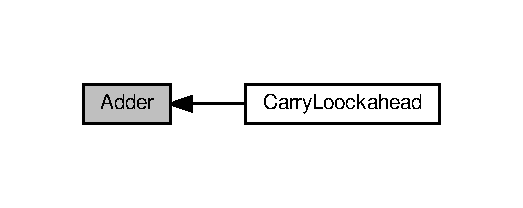
\includegraphics[width=251pt]{group___adder}
\end{center}
\end{figure}
\subsection*{Moduli}
\begin{DoxyCompactItemize}
\item 
\hyperlink{group___carry_loockahead}{Carry\+Loockahead}
\begin{DoxyCompactList}\small\item\em Addizionatore con carry-\/lookahead. \end{DoxyCompactList}\end{DoxyCompactItemize}
\subsection*{File}
\begin{DoxyCompactItemize}
\item 
file \hyperlink{cla__adder__cell_8vhd}{cla\+\_\+adder\+\_\+cell.\+vhd}
\end{DoxyCompactItemize}
\subsection*{Entities}
\begin{DoxyCompactItemize}
\item 
\hyperlink{classadder}{adder} entity
\item 
\hyperlink{classadder_1_1structural}{structural} architecture
\end{DoxyCompactItemize}
\subsection*{Components}
 \begin{DoxyCompactItemize}
\item 
\hyperlink{group___adder_gae7148956d4ef1d1cd14f35060634b9c3}{generic\+\_\+cla\+\_\+adder}  {\bfseries }  
\end{DoxyCompactItemize}
\subsection*{Generics}
 \begin{DoxyCompactItemize}
\item 
\hyperlink{group___adder_gae8451a648abadfad273ca1ae9b369657}{nbits} {\bfseries {\bfseries \textcolor{vhdlchar}{natural}\textcolor{vhdlchar}{ }\textcolor{vhdlchar}{ }\textcolor{vhdlchar}{\+:}\textcolor{vhdlchar}{=}\textcolor{vhdlchar}{ }\textcolor{vhdlchar}{ } \textcolor{vhdldigit}{8} \textcolor{vhdlchar}{ }}}
\item 
\hyperlink{group___adder_gadf05ca347ec6d3c85740dc697469b3db}{use\+\_\+custom} {\bfseries {\bfseries \textcolor{vhdlchar}{boolean}\textcolor{vhdlchar}{ }\textcolor{vhdlchar}{ }\textcolor{vhdlchar}{\+:}\textcolor{vhdlchar}{=}\textcolor{vhdlchar}{ }\textcolor{vhdlchar}{ }\textcolor{vhdlchar}{ }\textcolor{vhdlchar}{ }\textcolor{vhdlchar}{false}\textcolor{vhdlchar}{ }}}
\end{DoxyCompactItemize}
\subsection*{Ports}
 \begin{DoxyCompactItemize}
\item 
\hyperlink{group___adder_gad6ed6073f8ded668a403a0f7d85c53e8}{add1}  {\bfseries {\bfseries \textcolor{vhdlchar}{in}\textcolor{vhdlchar}{ }}} {\bfseries \textcolor{vhdlchar}{std\+\_\+logic\+\_\+vector}\textcolor{vhdlchar}{ }\textcolor{vhdlchar}{(}\textcolor{vhdlchar}{ }\textcolor{vhdlchar}{ }\textcolor{vhdlchar}{ }\textcolor{vhdlchar}{ }{\bfseries \hyperlink{group___adder_gae8451a648abadfad273ca1ae9b369657}{nbits}} \textcolor{vhdlchar}{-\/}\textcolor{vhdlchar}{ } \textcolor{vhdldigit}{1} \textcolor{vhdlchar}{ }\textcolor{vhdlchar}{downto}\textcolor{vhdlchar}{ }\textcolor{vhdlchar}{ } \textcolor{vhdldigit}{0} \textcolor{vhdlchar}{ }\textcolor{vhdlchar}{)}\textcolor{vhdlchar}{ }} 
\item 
\hyperlink{group___adder_gabf87ad241134c4d313c708910677575e}{add2}  {\bfseries {\bfseries \textcolor{vhdlchar}{in}\textcolor{vhdlchar}{ }}} {\bfseries \textcolor{vhdlchar}{std\+\_\+logic\+\_\+vector}\textcolor{vhdlchar}{ }\textcolor{vhdlchar}{(}\textcolor{vhdlchar}{ }\textcolor{vhdlchar}{ }\textcolor{vhdlchar}{ }\textcolor{vhdlchar}{ }{\bfseries \hyperlink{group___adder_gae8451a648abadfad273ca1ae9b369657}{nbits}} \textcolor{vhdlchar}{-\/}\textcolor{vhdlchar}{ } \textcolor{vhdldigit}{1} \textcolor{vhdlchar}{ }\textcolor{vhdlchar}{downto}\textcolor{vhdlchar}{ }\textcolor{vhdlchar}{ } \textcolor{vhdldigit}{0} \textcolor{vhdlchar}{ }\textcolor{vhdlchar}{)}\textcolor{vhdlchar}{ }} 
\item 
\hyperlink{group___adder_ga01f6ea3ddb4d1519676217bcb5959de8}{sum}  {\bfseries {\bfseries \textcolor{vhdlchar}{out}\textcolor{vhdlchar}{ }}} {\bfseries \textcolor{vhdlchar}{std\+\_\+logic\+\_\+vector}\textcolor{vhdlchar}{ }\textcolor{vhdlchar}{(}\textcolor{vhdlchar}{ }\textcolor{vhdlchar}{ }\textcolor{vhdlchar}{ }\textcolor{vhdlchar}{ }{\bfseries \hyperlink{group___adder_gae8451a648abadfad273ca1ae9b369657}{nbits}} \textcolor{vhdlchar}{-\/}\textcolor{vhdlchar}{ } \textcolor{vhdldigit}{1} \textcolor{vhdlchar}{ }\textcolor{vhdlchar}{downto}\textcolor{vhdlchar}{ }\textcolor{vhdlchar}{ } \textcolor{vhdldigit}{0} \textcolor{vhdlchar}{ }\textcolor{vhdlchar}{)}\textcolor{vhdlchar}{ }} 
\end{DoxyCompactItemize}


\subsection{Descrizione dettagliata}
Adder per la somma di due addendi con numero di bit variabile. 



\subsection{Documentazione delle variabili}
\hypertarget{group___adder_gad6ed6073f8ded668a403a0f7d85c53e8}{\index{Adder@{Adder}!add1@{add1}}
\index{add1@{add1}!Adder@{Adder}}
\subsubsection[{add1}]{\setlength{\rightskip}{0pt plus 5cm}{\bf add1} {\bfseries \textcolor{vhdlchar}{in}\textcolor{vhdlchar}{ }} {\bfseries \textcolor{vhdlchar}{std\+\_\+logic\+\_\+vector}\textcolor{vhdlchar}{ }\textcolor{vhdlchar}{(}\textcolor{vhdlchar}{ }\textcolor{vhdlchar}{ }\textcolor{vhdlchar}{ }\textcolor{vhdlchar}{ }{\bfseries {\bf nbits}} \textcolor{vhdlchar}{-\/}\textcolor{vhdlchar}{ } \textcolor{vhdldigit}{1} \textcolor{vhdlchar}{ }\textcolor{vhdlchar}{downto}\textcolor{vhdlchar}{ }\textcolor{vhdlchar}{ } \textcolor{vhdldigit}{0} \textcolor{vhdlchar}{ }\textcolor{vhdlchar}{)}\textcolor{vhdlchar}{ }} \hspace{0.3cm}{\ttfamily [Port]}}}\label{group___adder_gad6ed6073f8ded668a403a0f7d85c53e8}
\hypertarget{group___adder_gabf87ad241134c4d313c708910677575e}{\index{Adder@{Adder}!add2@{add2}}
\index{add2@{add2}!Adder@{Adder}}
\subsubsection[{add2}]{\setlength{\rightskip}{0pt plus 5cm}{\bf add2} {\bfseries \textcolor{vhdlchar}{in}\textcolor{vhdlchar}{ }} {\bfseries \textcolor{vhdlchar}{std\+\_\+logic\+\_\+vector}\textcolor{vhdlchar}{ }\textcolor{vhdlchar}{(}\textcolor{vhdlchar}{ }\textcolor{vhdlchar}{ }\textcolor{vhdlchar}{ }\textcolor{vhdlchar}{ }{\bfseries {\bf nbits}} \textcolor{vhdlchar}{-\/}\textcolor{vhdlchar}{ } \textcolor{vhdldigit}{1} \textcolor{vhdlchar}{ }\textcolor{vhdlchar}{downto}\textcolor{vhdlchar}{ }\textcolor{vhdlchar}{ } \textcolor{vhdldigit}{0} \textcolor{vhdlchar}{ }\textcolor{vhdlchar}{)}\textcolor{vhdlchar}{ }} \hspace{0.3cm}{\ttfamily [Port]}}}\label{group___adder_gabf87ad241134c4d313c708910677575e}
\hypertarget{group___adder_gae7148956d4ef1d1cd14f35060634b9c3}{\index{Adder@{Adder}!generic\+\_\+cla\+\_\+adder@{generic\+\_\+cla\+\_\+adder}}
\index{generic\+\_\+cla\+\_\+adder@{generic\+\_\+cla\+\_\+adder}!Adder@{Adder}}
\subsubsection[{generic\+\_\+cla\+\_\+adder}]{\setlength{\rightskip}{0pt plus 5cm}{\bf generic\+\_\+cla\+\_\+adder} {\bfseries \textcolor{vhdlchar}{ }} \hspace{0.3cm}{\ttfamily [Component]}}}\label{group___adder_gae7148956d4ef1d1cd14f35060634b9c3}
\hypertarget{group___adder_gae8451a648abadfad273ca1ae9b369657}{\index{Adder@{Adder}!nbits@{nbits}}
\index{nbits@{nbits}!Adder@{Adder}}
\subsubsection[{nbits}]{\setlength{\rightskip}{0pt plus 5cm}{\bf nbits} {\bfseries \textcolor{vhdlchar}{ }} {\bfseries \textcolor{vhdlchar}{natural}\textcolor{vhdlchar}{ }\textcolor{vhdlchar}{ }\textcolor{vhdlchar}{\+:}\textcolor{vhdlchar}{=}\textcolor{vhdlchar}{ }\textcolor{vhdlchar}{ } \textcolor{vhdldigit}{8} \textcolor{vhdlchar}{ }} \hspace{0.3cm}{\ttfamily [Generic]}}}\label{group___adder_gae8451a648abadfad273ca1ae9b369657}
\hypertarget{group___adder_ga01f6ea3ddb4d1519676217bcb5959de8}{\index{Adder@{Adder}!sum@{sum}}
\index{sum@{sum}!Adder@{Adder}}
\subsubsection[{sum}]{\setlength{\rightskip}{0pt plus 5cm}{\bf sum} {\bfseries \textcolor{vhdlchar}{out}\textcolor{vhdlchar}{ }} {\bfseries \textcolor{vhdlchar}{std\+\_\+logic\+\_\+vector}\textcolor{vhdlchar}{ }\textcolor{vhdlchar}{(}\textcolor{vhdlchar}{ }\textcolor{vhdlchar}{ }\textcolor{vhdlchar}{ }\textcolor{vhdlchar}{ }{\bfseries {\bf nbits}} \textcolor{vhdlchar}{-\/}\textcolor{vhdlchar}{ } \textcolor{vhdldigit}{1} \textcolor{vhdlchar}{ }\textcolor{vhdlchar}{downto}\textcolor{vhdlchar}{ }\textcolor{vhdlchar}{ } \textcolor{vhdldigit}{0} \textcolor{vhdlchar}{ }\textcolor{vhdlchar}{)}\textcolor{vhdlchar}{ }} \hspace{0.3cm}{\ttfamily [Port]}}}\label{group___adder_ga01f6ea3ddb4d1519676217bcb5959de8}
\hypertarget{group___adder_gadf05ca347ec6d3c85740dc697469b3db}{\index{Adder@{Adder}!use\+\_\+custom@{use\+\_\+custom}}
\index{use\+\_\+custom@{use\+\_\+custom}!Adder@{Adder}}
\subsubsection[{use\+\_\+custom}]{\setlength{\rightskip}{0pt plus 5cm}{\bf use\+\_\+custom} {\bfseries \textcolor{vhdlchar}{ }} {\bfseries \textcolor{vhdlchar}{boolean}\textcolor{vhdlchar}{ }\textcolor{vhdlchar}{ }\textcolor{vhdlchar}{\+:}\textcolor{vhdlchar}{=}\textcolor{vhdlchar}{ }\textcolor{vhdlchar}{ }\textcolor{vhdlchar}{ }\textcolor{vhdlchar}{ }\textcolor{vhdlchar}{false}\textcolor{vhdlchar}{ }} \hspace{0.3cm}{\ttfamily [Generic]}}}\label{group___adder_gadf05ca347ec6d3c85740dc697469b3db}

\hypertarget{group___carry_loockahead}{}\section{Carry\+Loockahead}
\label{group___carry_loockahead}\index{Carry\+Loockahead@{Carry\+Loockahead}}


Addizionatore con carry-\/lookahead.  


Diagramma di collaborazione per Carry\+Loockahead\+:\nopagebreak
\begin{figure}[H]
\begin{center}
\leavevmode
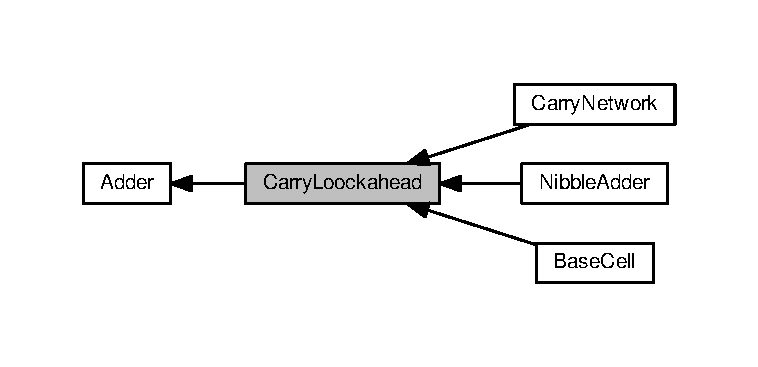
\includegraphics[width=350pt]{group___carry_loockahead}
\end{center}
\end{figure}
\subsection*{Moduli}
\begin{DoxyCompactItemize}
\item 
\hyperlink{group___base_cell}{Base\+Cell}
\begin{DoxyCompactList}\small\item\em Implementazione della cella base di un adder. \end{DoxyCompactList}\item 
\hyperlink{group___carry_network}{Carry\+Network}
\begin{DoxyCompactList}\small\item\em Rete di generazione dei segnali di carry per un adder a quattro bit. \end{DoxyCompactList}\item 
\hyperlink{group___nibble_adder}{Nibble\+Adder}
\begin{DoxyCompactList}\small\item\em Blocco elementare di somma a quattro bit. \end{DoxyCompactList}\end{DoxyCompactItemize}
\subsection*{Entities}
\begin{DoxyCompactItemize}
\item 
\hyperlink{classgeneric__cla__adder}{generic\+\_\+cla\+\_\+adder} entity
\begin{DoxyCompactList}\small\item\em Adder custom con carry-\/lookahead

\hyperlink{classgeneric__cla__adder}{generic\+\_\+cla\+\_\+adder} somma tra loro due addendi ed un carry in ingresso; gli addendi sono espressi su multipli interi di quattro bit. Oltre a generare la somma, genera il flag di carry ed il flag di overflow. \end{DoxyCompactList}\item 
\hyperlink{classgeneric__cla__adder_1_1structural}{structural} architecture
\begin{DoxyCompactList}\small\item\em Implementazione structural di \hyperlink{classgeneric__cla__adder}{generic\+\_\+cla\+\_\+adder}.

Questa implementazione istanzia tanti blocchi \hyperlink{classnibble__adder}{nibble\+\_\+adder} quanti siano i nibble in cui sono rappresentati gli addendi. La somma è espressa sullo stesso numero di bit. I diversi blocchi sono connessi tra loro come indicato nello schema ricordato di seguito\+: . \end{DoxyCompactList}\end{DoxyCompactItemize}
\subsection*{Components}
 \begin{DoxyCompactItemize}
\item 
\hyperlink{group___carry_loockahead_ga98a3a5b152caf0f2de1e31ac60088369}{nibble\+\_\+adder}  {\bfseries }  
\end{DoxyCompactItemize}
\subsection*{Generics}
 \begin{DoxyCompactItemize}
\item 
\hyperlink{group___carry_loockahead_ga0b63b586531492d0fa882246cca071c1}{nibbles} {\bfseries {\bfseries \textcolor{vhdlchar}{natural}\textcolor{vhdlchar}{ }\textcolor{vhdlchar}{ }\textcolor{vhdlchar}{\+:}\textcolor{vhdlchar}{=}\textcolor{vhdlchar}{ }\textcolor{vhdlchar}{ } \textcolor{vhdldigit}{2} \textcolor{vhdlchar}{ }}}
\end{DoxyCompactItemize}
\subsection*{Ports}
 \begin{DoxyCompactItemize}
\item 
\hyperlink{group___carry_loockahead_ga1c211cdf2d4cf97e869c442832c53439}{carry\+\_\+in}  {\bfseries {\bfseries \textcolor{vhdlchar}{in}\textcolor{vhdlchar}{ }}} {\bfseries \textcolor{vhdlchar}{std\+\_\+logic}\textcolor{vhdlchar}{ }} 
\item 
\hyperlink{group___carry_loockahead_gae4a2e124144a2f35270a55f0cf32a5ee}{addendum1}  {\bfseries {\bfseries \textcolor{vhdlchar}{in}\textcolor{vhdlchar}{ }}} {\bfseries \textcolor{vhdlchar}{std\+\_\+logic\+\_\+vector}\textcolor{vhdlchar}{ }\textcolor{vhdlchar}{(}\textcolor{vhdlchar}{ }\textcolor{vhdlchar}{(}\textcolor{vhdlchar}{ }\textcolor{vhdlchar}{ }\textcolor{vhdlchar}{ }\textcolor{vhdlchar}{ }{\bfseries \hyperlink{group___carry_loockahead_ga0b63b586531492d0fa882246cca071c1}{nibbles}} \textcolor{vhdlchar}{$\ast$}\textcolor{vhdlchar}{ } \textcolor{vhdldigit}{4} \textcolor{vhdlchar}{ }\textcolor{vhdlchar}{)}\textcolor{vhdlchar}{ }\textcolor{vhdlchar}{-\/}\textcolor{vhdlchar}{ } \textcolor{vhdldigit}{1} \textcolor{vhdlchar}{ }\textcolor{vhdlchar}{downto}\textcolor{vhdlchar}{ }\textcolor{vhdlchar}{ } \textcolor{vhdldigit}{0} \textcolor{vhdlchar}{ }\textcolor{vhdlchar}{)}\textcolor{vhdlchar}{ }} 
\begin{DoxyCompactList}\small\item\em addendo 1, espresso in complemento a due \end{DoxyCompactList}\item 
\hyperlink{group___carry_loockahead_ga2715463c615cf8418f85c6a1427ce62c}{addendum2}  {\bfseries {\bfseries \textcolor{vhdlchar}{in}\textcolor{vhdlchar}{ }}} {\bfseries \textcolor{vhdlchar}{std\+\_\+logic\+\_\+vector}\textcolor{vhdlchar}{ }\textcolor{vhdlchar}{(}\textcolor{vhdlchar}{ }\textcolor{vhdlchar}{(}\textcolor{vhdlchar}{ }\textcolor{vhdlchar}{ }\textcolor{vhdlchar}{ }\textcolor{vhdlchar}{ }{\bfseries \hyperlink{group___carry_loockahead_ga0b63b586531492d0fa882246cca071c1}{nibbles}} \textcolor{vhdlchar}{$\ast$}\textcolor{vhdlchar}{ } \textcolor{vhdldigit}{4} \textcolor{vhdlchar}{ }\textcolor{vhdlchar}{)}\textcolor{vhdlchar}{ }\textcolor{vhdlchar}{-\/}\textcolor{vhdlchar}{ } \textcolor{vhdldigit}{1} \textcolor{vhdlchar}{ }\textcolor{vhdlchar}{downto}\textcolor{vhdlchar}{ }\textcolor{vhdlchar}{ } \textcolor{vhdldigit}{0} \textcolor{vhdlchar}{ }\textcolor{vhdlchar}{)}\textcolor{vhdlchar}{ }} 
\begin{DoxyCompactList}\small\item\em addendo 2, espresso in complemento a due \end{DoxyCompactList}\item 
\hyperlink{group___carry_loockahead_ga1b4798a9e96bb32e9c08ce68e24e7871}{sum}  {\bfseries {\bfseries \textcolor{vhdlchar}{out}\textcolor{vhdlchar}{ }}} {\bfseries \textcolor{vhdlchar}{std\+\_\+logic\+\_\+vector}\textcolor{vhdlchar}{ }\textcolor{vhdlchar}{(}\textcolor{vhdlchar}{ }\textcolor{vhdlchar}{(}\textcolor{vhdlchar}{ }\textcolor{vhdlchar}{ }\textcolor{vhdlchar}{ }\textcolor{vhdlchar}{ }{\bfseries \hyperlink{group___carry_loockahead_ga0b63b586531492d0fa882246cca071c1}{nibbles}} \textcolor{vhdlchar}{$\ast$}\textcolor{vhdlchar}{ } \textcolor{vhdldigit}{4} \textcolor{vhdlchar}{ }\textcolor{vhdlchar}{)}\textcolor{vhdlchar}{ }\textcolor{vhdlchar}{-\/}\textcolor{vhdlchar}{ } \textcolor{vhdldigit}{1} \textcolor{vhdlchar}{ }\textcolor{vhdlchar}{downto}\textcolor{vhdlchar}{ }\textcolor{vhdlchar}{ } \textcolor{vhdldigit}{0} \textcolor{vhdlchar}{ }\textcolor{vhdlchar}{)}\textcolor{vhdlchar}{ }} 
\begin{DoxyCompactList}\small\item\em somma degli addendi, espressa in complemento a due \end{DoxyCompactList}\item 
\hyperlink{group___carry_loockahead_ga851aaea297bdc862fba5478c4bf0e214}{carry\+\_\+out}  {\bfseries {\bfseries \textcolor{vhdlchar}{out}\textcolor{vhdlchar}{ }}} {\bfseries \textcolor{vhdlchar}{std\+\_\+logic}\textcolor{vhdlchar}{ }} 
\item 
\hyperlink{group___carry_loockahead_ga9650307dde287e0bcfa1e26370c006c2}{overflow}  {\bfseries {\bfseries \textcolor{vhdlchar}{out}\textcolor{vhdlchar}{ }}} {\bfseries \textcolor{vhdlchar}{std\+\_\+logic}\textcolor{vhdlchar}{ }} 
\end{DoxyCompactItemize}
\subsection*{Signals}
 \begin{DoxyCompactItemize}
\item 
\hyperlink{group___carry_loockahead_ga19afe0b89973d7fc29362431f2e828b7}{prop} {\bfseries \textcolor{vhdlchar}{std\+\_\+logic\+\_\+vector}\textcolor{vhdlchar}{ }\textcolor{vhdlchar}{(}\textcolor{vhdlchar}{ }\textcolor{vhdlchar}{ } \textcolor{vhdldigit}{0} \textcolor{vhdlchar}{ }\textcolor{vhdlchar}{to}\textcolor{vhdlchar}{ }\textcolor{vhdlchar}{ }\textcolor{vhdlchar}{ }\textcolor{vhdlchar}{ }{\bfseries \hyperlink{group___carry_loockahead_ga0b63b586531492d0fa882246cca071c1}{nibbles}} \textcolor{vhdlchar}{ }\textcolor{vhdlchar}{)}\textcolor{vhdlchar}{ }} 
\item 
\hyperlink{group___carry_loockahead_ga7a68948b7b96c7b51036939fad8e71b3}{gen} {\bfseries \textcolor{vhdlchar}{std\+\_\+logic\+\_\+vector}\textcolor{vhdlchar}{ }\textcolor{vhdlchar}{(}\textcolor{vhdlchar}{ }\textcolor{vhdlchar}{ } \textcolor{vhdldigit}{0} \textcolor{vhdlchar}{ }\textcolor{vhdlchar}{to}\textcolor{vhdlchar}{ }\textcolor{vhdlchar}{ }\textcolor{vhdlchar}{ }\textcolor{vhdlchar}{ }{\bfseries \hyperlink{group___carry_loockahead_ga0b63b586531492d0fa882246cca071c1}{nibbles}} \textcolor{vhdlchar}{ }\textcolor{vhdlchar}{)}\textcolor{vhdlchar}{ }} 
\item 
\hyperlink{group___carry_loockahead_ga3c7f619aa6449e06bf0dd48a7db92b84}{sum\+\_\+tmp} {\bfseries \textcolor{vhdlchar}{std\+\_\+logic\+\_\+vector}\textcolor{vhdlchar}{ }\textcolor{vhdlchar}{(}\textcolor{vhdlchar}{ }\textcolor{vhdlchar}{(}\textcolor{vhdlchar}{ }\textcolor{vhdlchar}{ }\textcolor{vhdlchar}{ }\textcolor{vhdlchar}{ }{\bfseries \hyperlink{group___carry_loockahead_ga0b63b586531492d0fa882246cca071c1}{nibbles}} \textcolor{vhdlchar}{$\ast$}\textcolor{vhdlchar}{ } \textcolor{vhdldigit}{4} \textcolor{vhdlchar}{ }\textcolor{vhdlchar}{)}\textcolor{vhdlchar}{ }\textcolor{vhdlchar}{-\/}\textcolor{vhdlchar}{ } \textcolor{vhdldigit}{1} \textcolor{vhdlchar}{ }\textcolor{vhdlchar}{downto}\textcolor{vhdlchar}{ }\textcolor{vhdlchar}{ } \textcolor{vhdldigit}{0} \textcolor{vhdlchar}{ }\textcolor{vhdlchar}{)}\textcolor{vhdlchar}{ }} 
\end{DoxyCompactItemize}


\subsection{Descrizione dettagliata}
Addizionatore con carry-\/lookahead. 



\subsection{Documentazione delle variabili}
\index{Carry\+Loockahead@{Carry\+Loockahead}!addendum1@{addendum1}}
\index{addendum1@{addendum1}!Carry\+Loockahead@{Carry\+Loockahead}}
\subsubsection[{\texorpdfstring{addendum1}{addendum1}}]{\setlength{\rightskip}{0pt plus 5cm}{\bf addendum1} {\bfseries \textcolor{vhdlchar}{in}\textcolor{vhdlchar}{ }} {\bfseries \textcolor{vhdlchar}{std\+\_\+logic\+\_\+vector}\textcolor{vhdlchar}{ }\textcolor{vhdlchar}{(}\textcolor{vhdlchar}{ }\textcolor{vhdlchar}{(}\textcolor{vhdlchar}{ }\textcolor{vhdlchar}{ }\textcolor{vhdlchar}{ }\textcolor{vhdlchar}{ }{\bfseries {\bf nibbles}} \textcolor{vhdlchar}{$\ast$}\textcolor{vhdlchar}{ } \textcolor{vhdldigit}{4} \textcolor{vhdlchar}{ }\textcolor{vhdlchar}{)}\textcolor{vhdlchar}{ }\textcolor{vhdlchar}{-\/}\textcolor{vhdlchar}{ } \textcolor{vhdldigit}{1} \textcolor{vhdlchar}{ }\textcolor{vhdlchar}{downto}\textcolor{vhdlchar}{ }\textcolor{vhdlchar}{ } \textcolor{vhdldigit}{0} \textcolor{vhdlchar}{ }\textcolor{vhdlchar}{)}\textcolor{vhdlchar}{ }} \hspace{0.3cm}{\ttfamily [Port]}}\hypertarget{group___carry_loockahead_gae4a2e124144a2f35270a55f0cf32a5ee}{}\label{group___carry_loockahead_gae4a2e124144a2f35270a55f0cf32a5ee}


addendo 1, espresso in complemento a due 

segnale di \char`\"{}carry-\/in\char`\"{}, prodotto da un eventuale \hyperlink{classnibble__adder}{nibble\+\_\+adder} a monte; Può essere posto a \textquotesingle{}0\textquotesingle{} nel caso in cui non vi siano adder a monte. \index{Carry\+Loockahead@{Carry\+Loockahead}!addendum2@{addendum2}}
\index{addendum2@{addendum2}!Carry\+Loockahead@{Carry\+Loockahead}}
\subsubsection[{\texorpdfstring{addendum2}{addendum2}}]{\setlength{\rightskip}{0pt plus 5cm}{\bf addendum2} {\bfseries \textcolor{vhdlchar}{in}\textcolor{vhdlchar}{ }} {\bfseries \textcolor{vhdlchar}{std\+\_\+logic\+\_\+vector}\textcolor{vhdlchar}{ }\textcolor{vhdlchar}{(}\textcolor{vhdlchar}{ }\textcolor{vhdlchar}{(}\textcolor{vhdlchar}{ }\textcolor{vhdlchar}{ }\textcolor{vhdlchar}{ }\textcolor{vhdlchar}{ }{\bfseries {\bf nibbles}} \textcolor{vhdlchar}{$\ast$}\textcolor{vhdlchar}{ } \textcolor{vhdldigit}{4} \textcolor{vhdlchar}{ }\textcolor{vhdlchar}{)}\textcolor{vhdlchar}{ }\textcolor{vhdlchar}{-\/}\textcolor{vhdlchar}{ } \textcolor{vhdldigit}{1} \textcolor{vhdlchar}{ }\textcolor{vhdlchar}{downto}\textcolor{vhdlchar}{ }\textcolor{vhdlchar}{ } \textcolor{vhdldigit}{0} \textcolor{vhdlchar}{ }\textcolor{vhdlchar}{)}\textcolor{vhdlchar}{ }} \hspace{0.3cm}{\ttfamily [Port]}}\hypertarget{group___carry_loockahead_ga2715463c615cf8418f85c6a1427ce62c}{}\label{group___carry_loockahead_ga2715463c615cf8418f85c6a1427ce62c}


addendo 2, espresso in complemento a due 

\index{Carry\+Loockahead@{Carry\+Loockahead}!carry\+\_\+in@{carry\+\_\+in}}
\index{carry\+\_\+in@{carry\+\_\+in}!Carry\+Loockahead@{Carry\+Loockahead}}
\subsubsection[{\texorpdfstring{carry\+\_\+in}{carry_in}}]{\setlength{\rightskip}{0pt plus 5cm}{\bf carry\+\_\+in} {\bfseries \textcolor{vhdlchar}{in}\textcolor{vhdlchar}{ }} {\bfseries \textcolor{vhdlchar}{std\+\_\+logic}\textcolor{vhdlchar}{ }} \hspace{0.3cm}{\ttfamily [Port]}}\hypertarget{group___carry_loockahead_ga1c211cdf2d4cf97e869c442832c53439}{}\label{group___carry_loockahead_ga1c211cdf2d4cf97e869c442832c53439}
numero di nibble in cui sono rappresentati gli addendi e nel quale sarà espressa la somma degli stessi \index{Carry\+Loockahead@{Carry\+Loockahead}!carry\+\_\+out@{carry\+\_\+out}}
\index{carry\+\_\+out@{carry\+\_\+out}!Carry\+Loockahead@{Carry\+Loockahead}}
\subsubsection[{\texorpdfstring{carry\+\_\+out}{carry_out}}]{\setlength{\rightskip}{0pt plus 5cm}{\bf carry\+\_\+out} {\bfseries \textcolor{vhdlchar}{out}\textcolor{vhdlchar}{ }} {\bfseries \textcolor{vhdlchar}{std\+\_\+logic}\textcolor{vhdlchar}{ }} \hspace{0.3cm}{\ttfamily [Port]}}\hypertarget{group___carry_loockahead_ga851aaea297bdc862fba5478c4bf0e214}{}\label{group___carry_loockahead_ga851aaea297bdc862fba5478c4bf0e214}
\index{Carry\+Loockahead@{Carry\+Loockahead}!gen@{gen}}
\index{gen@{gen}!Carry\+Loockahead@{Carry\+Loockahead}}
\subsubsection[{\texorpdfstring{gen}{gen}}]{\setlength{\rightskip}{0pt plus 5cm}{\bf gen} {\bfseries \textcolor{vhdlchar}{std\+\_\+logic\+\_\+vector}\textcolor{vhdlchar}{ }\textcolor{vhdlchar}{(}\textcolor{vhdlchar}{ }\textcolor{vhdlchar}{ } \textcolor{vhdldigit}{0} \textcolor{vhdlchar}{ }\textcolor{vhdlchar}{to}\textcolor{vhdlchar}{ }\textcolor{vhdlchar}{ }\textcolor{vhdlchar}{ }\textcolor{vhdlchar}{ }{\bfseries {\bf nibbles}} \textcolor{vhdlchar}{ }\textcolor{vhdlchar}{)}\textcolor{vhdlchar}{ }} \hspace{0.3cm}{\ttfamily [Signal]}}\hypertarget{group___carry_loockahead_ga7a68948b7b96c7b51036939fad8e71b3}{}\label{group___carry_loockahead_ga7a68948b7b96c7b51036939fad8e71b3}
funzione \char`\"{}propagazione\char`\"{} del carry, prodotta dai diversi blocchi \hyperlink{classnibble__adder}{nibble\+\_\+adder}; prop(i) vale 1 quando, sulla base degli ingressi, l\textquotesingle{}i-\/esimo \hyperlink{classnibble__adder}{nibble\+\_\+adder} propaghera\textquotesingle{} un eventuale carry in ingresso; prop(0) = \textquotesingle{}1\textquotesingle{}; \index{Carry\+Loockahead@{Carry\+Loockahead}!nibble\+\_\+adder@{nibble\+\_\+adder}}
\index{nibble\+\_\+adder@{nibble\+\_\+adder}!Carry\+Loockahead@{Carry\+Loockahead}}
\subsubsection[{\texorpdfstring{nibble\+\_\+adder}{nibble_adder}}]{\setlength{\rightskip}{0pt plus 5cm}{\bf nibble\+\_\+adder} {\bfseries \textcolor{vhdlchar}{ }} \hspace{0.3cm}{\ttfamily [Component]}}\hypertarget{group___carry_loockahead_ga98a3a5b152caf0f2de1e31ac60088369}{}\label{group___carry_loockahead_ga98a3a5b152caf0f2de1e31ac60088369}
\index{Carry\+Loockahead@{Carry\+Loockahead}!nibbles@{nibbles}}
\index{nibbles@{nibbles}!Carry\+Loockahead@{Carry\+Loockahead}}
\subsubsection[{\texorpdfstring{nibbles}{nibbles}}]{\setlength{\rightskip}{0pt plus 5cm}{\bf nibbles} {\bfseries \textcolor{vhdlchar}{ }} {\bfseries \textcolor{vhdlchar}{natural}\textcolor{vhdlchar}{ }\textcolor{vhdlchar}{ }\textcolor{vhdlchar}{\+:}\textcolor{vhdlchar}{=}\textcolor{vhdlchar}{ }\textcolor{vhdlchar}{ } \textcolor{vhdldigit}{2} \textcolor{vhdlchar}{ }} \hspace{0.3cm}{\ttfamily [Generic]}}\hypertarget{group___carry_loockahead_ga0b63b586531492d0fa882246cca071c1}{}\label{group___carry_loockahead_ga0b63b586531492d0fa882246cca071c1}
\index{Carry\+Loockahead@{Carry\+Loockahead}!overflow@{overflow}}
\index{overflow@{overflow}!Carry\+Loockahead@{Carry\+Loockahead}}
\subsubsection[{\texorpdfstring{overflow}{overflow}}]{\setlength{\rightskip}{0pt plus 5cm}{\bf overflow} {\bfseries \textcolor{vhdlchar}{out}\textcolor{vhdlchar}{ }} {\bfseries \textcolor{vhdlchar}{std\+\_\+logic}\textcolor{vhdlchar}{ }} \hspace{0.3cm}{\ttfamily [Port]}}\hypertarget{group___carry_loockahead_ga9650307dde287e0bcfa1e26370c006c2}{}\label{group___carry_loockahead_ga9650307dde287e0bcfa1e26370c006c2}
carry in uscita; viene calcolato come carry\+\_\+out=gen(nibbles)+(prop(nibbles)$\ast$carry\+\_\+in), dove gen(nibbles) e prop(nibbles) sono, rispettivamente, la funzione \char`\"{}generazione\char`\"{} e \char`\"{}propagazione\char`\"{} del carry prodotta dall\textquotesingle{}ultimo blocco \hyperlink{classnibble__adder}{nibble\+\_\+adder}, cioè quello che somma i nibble di peso massimo, e carry\+\_\+in e\textquotesingle{} il carry in ingresso al sommatore. \index{Carry\+Loockahead@{Carry\+Loockahead}!prop@{prop}}
\index{prop@{prop}!Carry\+Loockahead@{Carry\+Loockahead}}
\subsubsection[{\texorpdfstring{prop}{prop}}]{\setlength{\rightskip}{0pt plus 5cm}{\bf prop} {\bfseries \textcolor{vhdlchar}{std\+\_\+logic\+\_\+vector}\textcolor{vhdlchar}{ }\textcolor{vhdlchar}{(}\textcolor{vhdlchar}{ }\textcolor{vhdlchar}{ } \textcolor{vhdldigit}{0} \textcolor{vhdlchar}{ }\textcolor{vhdlchar}{to}\textcolor{vhdlchar}{ }\textcolor{vhdlchar}{ }\textcolor{vhdlchar}{ }\textcolor{vhdlchar}{ }{\bfseries {\bf nibbles}} \textcolor{vhdlchar}{ }\textcolor{vhdlchar}{)}\textcolor{vhdlchar}{ }} \hspace{0.3cm}{\ttfamily [Signal]}}\hypertarget{group___carry_loockahead_ga19afe0b89973d7fc29362431f2e828b7}{}\label{group___carry_loockahead_ga19afe0b89973d7fc29362431f2e828b7}
\index{Carry\+Loockahead@{Carry\+Loockahead}!sum@{sum}}
\index{sum@{sum}!Carry\+Loockahead@{Carry\+Loockahead}}
\subsubsection[{\texorpdfstring{sum}{sum}}]{\setlength{\rightskip}{0pt plus 5cm}{\bf sum} {\bfseries \textcolor{vhdlchar}{out}\textcolor{vhdlchar}{ }} {\bfseries \textcolor{vhdlchar}{std\+\_\+logic\+\_\+vector}\textcolor{vhdlchar}{ }\textcolor{vhdlchar}{(}\textcolor{vhdlchar}{ }\textcolor{vhdlchar}{(}\textcolor{vhdlchar}{ }\textcolor{vhdlchar}{ }\textcolor{vhdlchar}{ }\textcolor{vhdlchar}{ }{\bfseries {\bf nibbles}} \textcolor{vhdlchar}{$\ast$}\textcolor{vhdlchar}{ } \textcolor{vhdldigit}{4} \textcolor{vhdlchar}{ }\textcolor{vhdlchar}{)}\textcolor{vhdlchar}{ }\textcolor{vhdlchar}{-\/}\textcolor{vhdlchar}{ } \textcolor{vhdldigit}{1} \textcolor{vhdlchar}{ }\textcolor{vhdlchar}{downto}\textcolor{vhdlchar}{ }\textcolor{vhdlchar}{ } \textcolor{vhdldigit}{0} \textcolor{vhdlchar}{ }\textcolor{vhdlchar}{)}\textcolor{vhdlchar}{ }} \hspace{0.3cm}{\ttfamily [Port]}}\hypertarget{group___carry_loockahead_ga1b4798a9e96bb32e9c08ce68e24e7871}{}\label{group___carry_loockahead_ga1b4798a9e96bb32e9c08ce68e24e7871}


somma degli addendi, espressa in complemento a due 

\index{Carry\+Loockahead@{Carry\+Loockahead}!sum\+\_\+tmp@{sum\+\_\+tmp}}
\index{sum\+\_\+tmp@{sum\+\_\+tmp}!Carry\+Loockahead@{Carry\+Loockahead}}
\subsubsection[{\texorpdfstring{sum\+\_\+tmp}{sum_tmp}}]{\setlength{\rightskip}{0pt plus 5cm}{\bf sum\+\_\+tmp} {\bfseries \textcolor{vhdlchar}{std\+\_\+logic\+\_\+vector}\textcolor{vhdlchar}{ }\textcolor{vhdlchar}{(}\textcolor{vhdlchar}{ }\textcolor{vhdlchar}{(}\textcolor{vhdlchar}{ }\textcolor{vhdlchar}{ }\textcolor{vhdlchar}{ }\textcolor{vhdlchar}{ }{\bfseries {\bf nibbles}} \textcolor{vhdlchar}{$\ast$}\textcolor{vhdlchar}{ } \textcolor{vhdldigit}{4} \textcolor{vhdlchar}{ }\textcolor{vhdlchar}{)}\textcolor{vhdlchar}{ }\textcolor{vhdlchar}{-\/}\textcolor{vhdlchar}{ } \textcolor{vhdldigit}{1} \textcolor{vhdlchar}{ }\textcolor{vhdlchar}{downto}\textcolor{vhdlchar}{ }\textcolor{vhdlchar}{ } \textcolor{vhdldigit}{0} \textcolor{vhdlchar}{ }\textcolor{vhdlchar}{)}\textcolor{vhdlchar}{ }} \hspace{0.3cm}{\ttfamily [Signal]}}\hypertarget{group___carry_loockahead_ga3c7f619aa6449e06bf0dd48a7db92b84}{}\label{group___carry_loockahead_ga3c7f619aa6449e06bf0dd48a7db92b84}
funzione \char`\"{}generazione\char`\"{} del carry, prodotta dai diversi blocchi \hyperlink{classnibble__adder}{nibble\+\_\+adder}; gen(i) vale 1 quando, sulla base degli ingressi, l\textquotesingle{}i-\/esimo \hyperlink{classnibble__adder}{nibble\+\_\+adder} genera carry in uscita; gen(0) = \textquotesingle{}0\textquotesingle{}; 
\hypertarget{group___base_cell}{}\section{Base\+Cell}
\label{group___base_cell}\index{Base\+Cell@{Base\+Cell}}


Implementazione della cella base di un adder.  


Diagramma di collaborazione per Base\+Cell\+:\nopagebreak
\begin{figure}[H]
\begin{center}
\leavevmode
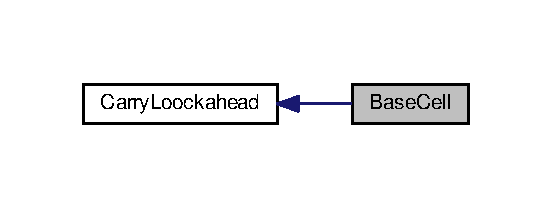
\includegraphics[width=265pt]{group___base_cell}
\end{center}
\end{figure}
\subsection*{Entities}
\begin{DoxyCompactItemize}
\item 
\hyperlink{classcla__adder__cell}{cla\+\_\+adder\+\_\+cell} entity
\begin{DoxyCompactList}\small\item\em Cella base di un addizionatore con carry-\/lookahead.

La cella somma tra loro due addendi ed un carry in ingresso, tutti espressi su un solo bit. Oltre a generare la somma, genera le funzioni \char`\"{}propagazione\char`\"{} e \char`\"{}generazione\char`\"{} del carry. \end{DoxyCompactList}\item 
\hyperlink{classcla__adder__cell_1_1dataflow}{dataflow} architecture
\end{DoxyCompactItemize}
\subsection*{Ports}
 \begin{DoxyCompactItemize}
\item 
\hyperlink{group___base_cell_ga2b16ee1ce0d8ffb8f85ccea13f8ba38d}{add1}  {\bfseries {\bfseries \textcolor{vhdlchar}{in}\textcolor{vhdlchar}{ }}} {\bfseries \textcolor{vhdlchar}{std\+\_\+logic}\textcolor{vhdlchar}{ }} 
\begin{DoxyCompactList}\small\item\em addendo 1 \end{DoxyCompactList}\item 
\hyperlink{group___base_cell_gac3ebb689e34fc5e7657726b18d8b5369}{add2}  {\bfseries {\bfseries \textcolor{vhdlchar}{in}\textcolor{vhdlchar}{ }}} {\bfseries \textcolor{vhdlchar}{std\+\_\+logic}\textcolor{vhdlchar}{ }} 
\begin{DoxyCompactList}\small\item\em addendo 2 \end{DoxyCompactList}\item 
\hyperlink{group___base_cell_gaa556a73dc4a4de1a0d662b25adbcbe33}{carryin}  {\bfseries {\bfseries \textcolor{vhdlchar}{in}\textcolor{vhdlchar}{ }}} {\bfseries \textcolor{vhdlchar}{std\+\_\+logic}\textcolor{vhdlchar}{ }} 
\begin{DoxyCompactList}\small\item\em carry in ingresso \end{DoxyCompactList}\item 
\hyperlink{group___base_cell_gac94466f3a0e3e34f0231abcf4b667ade}{prop}  {\bfseries {\bfseries \textcolor{vhdlchar}{out}\textcolor{vhdlchar}{ }}} {\bfseries \textcolor{vhdlchar}{std\+\_\+logic}\textcolor{vhdlchar}{ }} 
\item 
\hyperlink{group___base_cell_gaad65a9c9ebd4dd83c2835249a1ba2dff}{gen}  {\bfseries {\bfseries \textcolor{vhdlchar}{out}\textcolor{vhdlchar}{ }}} {\bfseries \textcolor{vhdlchar}{std\+\_\+logic}\textcolor{vhdlchar}{ }} 
\item 
\hyperlink{group___base_cell_ga0d9fc1b21b42422b12d68ad73ca8ef13}{sum}  {\bfseries {\bfseries \textcolor{vhdlchar}{out}\textcolor{vhdlchar}{ }}} {\bfseries \textcolor{vhdlchar}{std\+\_\+logic}\textcolor{vhdlchar}{ }} 
\end{DoxyCompactItemize}


\subsection{Descrizione dettagliata}
Implementazione della cella base di un adder. 



\subsection{Documentazione delle variabili}
\index{Base\+Cell@{Base\+Cell}!add1@{add1}}
\index{add1@{add1}!Base\+Cell@{Base\+Cell}}
\subsubsection[{\texorpdfstring{add1}{add1}}]{\setlength{\rightskip}{0pt plus 5cm}{\bf add1} {\bfseries \textcolor{vhdlchar}{in}\textcolor{vhdlchar}{ }} {\bfseries \textcolor{vhdlchar}{std\+\_\+logic}\textcolor{vhdlchar}{ }} \hspace{0.3cm}{\ttfamily [Port]}}\hypertarget{group___base_cell_ga2b16ee1ce0d8ffb8f85ccea13f8ba38d}{}\label{group___base_cell_ga2b16ee1ce0d8ffb8f85ccea13f8ba38d}


addendo 1 

\index{Base\+Cell@{Base\+Cell}!add2@{add2}}
\index{add2@{add2}!Base\+Cell@{Base\+Cell}}
\subsubsection[{\texorpdfstring{add2}{add2}}]{\setlength{\rightskip}{0pt plus 5cm}{\bf add2} {\bfseries \textcolor{vhdlchar}{in}\textcolor{vhdlchar}{ }} {\bfseries \textcolor{vhdlchar}{std\+\_\+logic}\textcolor{vhdlchar}{ }} \hspace{0.3cm}{\ttfamily [Port]}}\hypertarget{group___base_cell_gac3ebb689e34fc5e7657726b18d8b5369}{}\label{group___base_cell_gac3ebb689e34fc5e7657726b18d8b5369}


addendo 2 

\index{Base\+Cell@{Base\+Cell}!carryin@{carryin}}
\index{carryin@{carryin}!Base\+Cell@{Base\+Cell}}
\subsubsection[{\texorpdfstring{carryin}{carryin}}]{\setlength{\rightskip}{0pt plus 5cm}{\bf carryin} {\bfseries \textcolor{vhdlchar}{in}\textcolor{vhdlchar}{ }} {\bfseries \textcolor{vhdlchar}{std\+\_\+logic}\textcolor{vhdlchar}{ }} \hspace{0.3cm}{\ttfamily [Port]}}\hypertarget{group___base_cell_gaa556a73dc4a4de1a0d662b25adbcbe33}{}\label{group___base_cell_gaa556a73dc4a4de1a0d662b25adbcbe33}


carry in ingresso 

\index{Base\+Cell@{Base\+Cell}!gen@{gen}}
\index{gen@{gen}!Base\+Cell@{Base\+Cell}}
\subsubsection[{\texorpdfstring{gen}{gen}}]{\setlength{\rightskip}{0pt plus 5cm}{\bf gen} {\bfseries \textcolor{vhdlchar}{out}\textcolor{vhdlchar}{ }} {\bfseries \textcolor{vhdlchar}{std\+\_\+logic}\textcolor{vhdlchar}{ }} \hspace{0.3cm}{\ttfamily [Port]}}\hypertarget{group___base_cell_gaad65a9c9ebd4dd83c2835249a1ba2dff}{}\label{group___base_cell_gaad65a9c9ebd4dd83c2835249a1ba2dff}
funzione "propagazione”, vale 1 quando, sulla base degli ingressi, un adder propaghera\textquotesingle{} un eventuale carry in ingresso; prop = add1 OR add2 \index{Base\+Cell@{Base\+Cell}!prop@{prop}}
\index{prop@{prop}!Base\+Cell@{Base\+Cell}}
\subsubsection[{\texorpdfstring{prop}{prop}}]{\setlength{\rightskip}{0pt plus 5cm}{\bf prop} {\bfseries \textcolor{vhdlchar}{out}\textcolor{vhdlchar}{ }} {\bfseries \textcolor{vhdlchar}{std\+\_\+logic}\textcolor{vhdlchar}{ }} \hspace{0.3cm}{\ttfamily [Port]}}\hypertarget{group___base_cell_gac94466f3a0e3e34f0231abcf4b667ade}{}\label{group___base_cell_gac94466f3a0e3e34f0231abcf4b667ade}
\index{Base\+Cell@{Base\+Cell}!sum@{sum}}
\index{sum@{sum}!Base\+Cell@{Base\+Cell}}
\subsubsection[{\texorpdfstring{sum}{sum}}]{\setlength{\rightskip}{0pt plus 5cm}{\bf sum} {\bfseries \textcolor{vhdlchar}{out}\textcolor{vhdlchar}{ }} {\bfseries \textcolor{vhdlchar}{std\+\_\+logic}\textcolor{vhdlchar}{ }} \hspace{0.3cm}{\ttfamily [Port]}}\hypertarget{group___base_cell_ga0d9fc1b21b42422b12d68ad73ca8ef13}{}\label{group___base_cell_ga0d9fc1b21b42422b12d68ad73ca8ef13}
funzione "generazione”, vale 1 quando, sulla base degli ingressi, un adder generera\textquotesingle{} riporto; gen = add1 A\+ND add2; 
\hypertarget{group___carry_network}{}\section{Carry\+Network}
\label{group___carry_network}\index{Carry\+Network@{Carry\+Network}}


Rete di generazione dei segnali di carry per un adder a quattro bit.  


Diagramma di collaborazione per Carry\+Network\+:\nopagebreak
\begin{figure}[H]
\begin{center}
\leavevmode
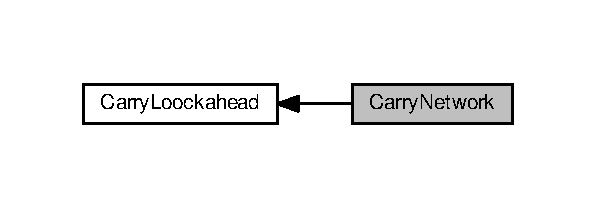
\includegraphics[width=286pt]{group___carry_network}
\end{center}
\end{figure}
\subsection*{Entities}
\begin{DoxyCompactItemize}
\item 
\hyperlink{classcla__carry__net}{cla\+\_\+carry\+\_\+net} entity
\begin{DoxyCompactList}\small\item\em Rete logica di calcolo dei riporti per un addizionatore a quattro bit con carry lookahead.

Permette di anticipare il calcolo dei riporti usando le funzioni \char`\"{}propagazione\char`\"{} e \char`\"{}generazione\char`\"{} prodotte dai singoli blocchi \hyperlink{classcla__adder__cell}{cla\+\_\+adder\+\_\+cell}, in modo da ridurre tempo necessario ad effettuare il calcolo di tutti i carry, quindi il tempo necessario a completare la somma. Questo blocco calcola solo i carry, pertanto va connesso ai blocchi \hyperlink{classcla__adder__cell}{cla\+\_\+adder\+\_\+cell}, per il calcolo materiale della somma, così come indicato dallo schema seguente, il quale rappresenta lo schema completo di un addizionatore a quattro bit\+: . \end{DoxyCompactList}\item 
\hyperlink{classcla__carry__net_1_1dataflow}{dataflow} architecture
\begin{DoxyCompactList}\small\item\em Implementazione dataflow dell\textquotesingle{}entita\textquotesingle{} \hyperlink{classcla__carry__net}{cla\+\_\+carry\+\_\+net}.

L\textquotesingle{}implementazione si basa sul seguente ragionamento\+: Proviamo ad esprimere, adesso, il carry carryout(i+1) in base alle funzioni gen(i) e prop(i), partendo, ad esempio, da carryout(1). Il carry carryout(0) varra\textquotesingle{} 1 se al passo precedente è stato generato riporto oppure se verra\textquotesingle{} propagato il carry carryin. In formule\+: \begin{center}carryout(0)=genin+(propin$\ast$carryin);\end{center}  Possiamo estendere lo stesso ragionamento a carryout(2)\+: \begin{center}carryout(1)=gen(1)+prop(1)$\ast$carryout(1)=gen(1)+prop(1)$\ast$gen(0)+prop(1)$\ast$prop(0)$\ast$carryin\end{center}  Cio\textquotesingle{} significa che il riporto carryout(1) lo si può esprimere sulla base di soli dati di ingresso con reti combinatorie a due livelli, senza utilizzare valori calcolati da nodi precedenti. Tutto ciò si traduce in un minor tempo necessario ad effettuare il calcolo di tutti i carry, quindi un minor tempo necessario a completare la somma. Purtroppo non si può procedere in questo modo ad oltranza per cui si tende a spezzare" la rete per il calcolo dei carry in blocchi più piccoli, ad esempio reti per il calcolo di carry per quattro bit. Considerando che \begin{center}carryout(4)=gen(3)+prop(3)$\ast$carryout(3)=...=genout+propout$\ast$carryin\end{center}  con \begin{center}genout=gen(3)+(prop(3)$\ast$gen(2))+(prop(3)$\ast$prop(2)$\ast$gen(1))+(prop(3)$\ast$prop(2)$\ast$prop(1)$\ast$gen(0))+(prop(3)$\ast$prop(2)$\ast$prop(1)$\ast$prop(0)$\ast$genin)\end{center}  \begin{center}propout=prop(3)$\ast$prop(2)$\ast$prop(1)$\ast$prop(0)$\ast$propin\end{center}  Si può costruire dei blocchi che presentino in uscita i segnali genout e propout, in modo da permettere ad eventuali blocchi successivi il calcolo veloce dei carry sulla base di questi segnali e del segnale carryin. \end{DoxyCompactList}\end{DoxyCompactItemize}
\subsection*{Ports}
 \begin{DoxyCompactItemize}
\item 
\hyperlink{group___carry_network_gac1f84cd3374a5a4d2ee2669ebdadafe8}{prop}  {\bfseries {\bfseries \textcolor{vhdlchar}{in}\textcolor{vhdlchar}{ }}} {\bfseries \textcolor{vhdlchar}{std\+\_\+logic\+\_\+vector}\textcolor{vhdlchar}{ }\textcolor{vhdlchar}{(}\textcolor{vhdlchar}{ }\textcolor{vhdlchar}{ } \textcolor{vhdldigit}{3} \textcolor{vhdlchar}{ }\textcolor{vhdlchar}{downto}\textcolor{vhdlchar}{ }\textcolor{vhdlchar}{ } \textcolor{vhdldigit}{0} \textcolor{vhdlchar}{ }\textcolor{vhdlchar}{)}\textcolor{vhdlchar}{ }} 
\item 
\hyperlink{group___carry_network_ga1ff97daaf4e03defc21748593cacfaa7}{gen}  {\bfseries {\bfseries \textcolor{vhdlchar}{in}\textcolor{vhdlchar}{ }}} {\bfseries \textcolor{vhdlchar}{std\+\_\+logic\+\_\+vector}\textcolor{vhdlchar}{ }\textcolor{vhdlchar}{(}\textcolor{vhdlchar}{ }\textcolor{vhdlchar}{ } \textcolor{vhdldigit}{3} \textcolor{vhdlchar}{ }\textcolor{vhdlchar}{downto}\textcolor{vhdlchar}{ }\textcolor{vhdlchar}{ } \textcolor{vhdldigit}{0} \textcolor{vhdlchar}{ }\textcolor{vhdlchar}{)}\textcolor{vhdlchar}{ }} 
\item 
\hyperlink{group___carry_network_gaa556a73dc4a4de1a0d662b25adbcbe33}{carryin}  {\bfseries {\bfseries \textcolor{vhdlchar}{in}\textcolor{vhdlchar}{ }}} {\bfseries \textcolor{vhdlchar}{std\+\_\+logic}\textcolor{vhdlchar}{ }} 
\begin{DoxyCompactList}\small\item\em segnale di \char`\"{}carry-\/in\char`\"{}, prodotto da un eventuale \hyperlink{classcla__carry__net}{cla\+\_\+carry\+\_\+net} a monte. \end{DoxyCompactList}\item 
\hyperlink{group___carry_network_ga422e8e7ee01fc7ac7b7390cd2ad8c87b}{propin}  {\bfseries {\bfseries \textcolor{vhdlchar}{in}\textcolor{vhdlchar}{ }}} {\bfseries \textcolor{vhdlchar}{std\+\_\+logic}\textcolor{vhdlchar}{ }} 
\begin{DoxyCompactList}\small\item\em funzione \char`\"{}propagazione\char`\"{}, prodotta da una eventuale \hyperlink{classcla__carry__net}{cla\+\_\+carry\+\_\+net} a monte \end{DoxyCompactList}\item 
\hyperlink{group___carry_network_ga0a46d5193cb73eb993bc5d4f69741d0a}{genin}  {\bfseries {\bfseries \textcolor{vhdlchar}{in}\textcolor{vhdlchar}{ }}} {\bfseries \textcolor{vhdlchar}{std\+\_\+logic}\textcolor{vhdlchar}{ }} 
\begin{DoxyCompactList}\small\item\em funzione \char`\"{}generazione\char`\"{}, prodotta da una eventuale \hyperlink{classcla__carry__net}{cla\+\_\+carry\+\_\+net} a monte \end{DoxyCompactList}\item 
\hyperlink{group___carry_network_ga6b265f3fe41195485dfedd9824c3598f}{carryout}  {\bfseries {\bfseries \textcolor{vhdlchar}{out}\textcolor{vhdlchar}{ }}} {\bfseries \textcolor{vhdlchar}{std\+\_\+logic\+\_\+vector}\textcolor{vhdlchar}{ }\textcolor{vhdlchar}{(}\textcolor{vhdlchar}{ }\textcolor{vhdlchar}{ } \textcolor{vhdldigit}{3} \textcolor{vhdlchar}{ }\textcolor{vhdlchar}{downto}\textcolor{vhdlchar}{ }\textcolor{vhdlchar}{ } \textcolor{vhdldigit}{0} \textcolor{vhdlchar}{ }\textcolor{vhdlchar}{)}\textcolor{vhdlchar}{ }} 
\item 
\hyperlink{group___carry_network_ga5957c9cdd706cafd2da8855133a002c9}{propout}  {\bfseries {\bfseries \textcolor{vhdlchar}{out}\textcolor{vhdlchar}{ }}} {\bfseries \textcolor{vhdlchar}{std\+\_\+logic}\textcolor{vhdlchar}{ }} 
\item 
\hyperlink{group___carry_network_ga068cd5c4d23e284cb942702252ed1491}{genout}  {\bfseries {\bfseries \textcolor{vhdlchar}{out}\textcolor{vhdlchar}{ }}} {\bfseries \textcolor{vhdlchar}{std\+\_\+logic}\textcolor{vhdlchar}{ }} 
\end{DoxyCompactItemize}


\subsection{Descrizione dettagliata}
Rete di generazione dei segnali di carry per un adder a quattro bit. 



\subsection{Documentazione delle variabili}
\index{Carry\+Network@{Carry\+Network}!carryin@{carryin}}
\index{carryin@{carryin}!Carry\+Network@{Carry\+Network}}
\subsubsection[{\texorpdfstring{carryin}{carryin}}]{\setlength{\rightskip}{0pt plus 5cm}{\bf carryin} {\bfseries \textcolor{vhdlchar}{in}\textcolor{vhdlchar}{ }} {\bfseries \textcolor{vhdlchar}{std\+\_\+logic}\textcolor{vhdlchar}{ }} \hspace{0.3cm}{\ttfamily [Port]}}\hypertarget{group___carry_network_gaa556a73dc4a4de1a0d662b25adbcbe33}{}\label{group___carry_network_gaa556a73dc4a4de1a0d662b25adbcbe33}


segnale di \char`\"{}carry-\/in\char`\"{}, prodotto da un eventuale \hyperlink{classcla__carry__net}{cla\+\_\+carry\+\_\+net} a monte. 

funzione \char`\"{}generazione\char`\"{} prodotta da \hyperlink{classcla__adder__cell}{cla\+\_\+adder\+\_\+cell}; vale 1 quando, sulla base degli ingressi, un adder generera\textquotesingle{} un carry in uscita; gen(i) = add(i) A\+ND add(i); in questo caso viene prodotta da quattro blocchi \hyperlink{classcla__adder__cell}{cla\+\_\+adder\+\_\+cell} sulla base dei loro ingressi \index{Carry\+Network@{Carry\+Network}!carryout@{carryout}}
\index{carryout@{carryout}!Carry\+Network@{Carry\+Network}}
\subsubsection[{\texorpdfstring{carryout}{carryout}}]{\setlength{\rightskip}{0pt plus 5cm}{\bf carryout} {\bfseries \textcolor{vhdlchar}{out}\textcolor{vhdlchar}{ }} {\bfseries \textcolor{vhdlchar}{std\+\_\+logic\+\_\+vector}\textcolor{vhdlchar}{ }\textcolor{vhdlchar}{(}\textcolor{vhdlchar}{ }\textcolor{vhdlchar}{ } \textcolor{vhdldigit}{3} \textcolor{vhdlchar}{ }\textcolor{vhdlchar}{downto}\textcolor{vhdlchar}{ }\textcolor{vhdlchar}{ } \textcolor{vhdldigit}{0} \textcolor{vhdlchar}{ }\textcolor{vhdlchar}{)}\textcolor{vhdlchar}{ }} \hspace{0.3cm}{\ttfamily [Port]}}\hypertarget{group___carry_network_ga6b265f3fe41195485dfedd9824c3598f}{}\label{group___carry_network_ga6b265f3fe41195485dfedd9824c3598f}
\index{Carry\+Network@{Carry\+Network}!gen@{gen}}
\index{gen@{gen}!Carry\+Network@{Carry\+Network}}
\subsubsection[{\texorpdfstring{gen}{gen}}]{\setlength{\rightskip}{0pt plus 5cm}{\bf gen} {\bfseries \textcolor{vhdlchar}{in}\textcolor{vhdlchar}{ }} {\bfseries \textcolor{vhdlchar}{std\+\_\+logic\+\_\+vector}\textcolor{vhdlchar}{ }\textcolor{vhdlchar}{(}\textcolor{vhdlchar}{ }\textcolor{vhdlchar}{ } \textcolor{vhdldigit}{3} \textcolor{vhdlchar}{ }\textcolor{vhdlchar}{downto}\textcolor{vhdlchar}{ }\textcolor{vhdlchar}{ } \textcolor{vhdldigit}{0} \textcolor{vhdlchar}{ }\textcolor{vhdlchar}{)}\textcolor{vhdlchar}{ }} \hspace{0.3cm}{\ttfamily [Port]}}\hypertarget{group___carry_network_ga1ff97daaf4e03defc21748593cacfaa7}{}\label{group___carry_network_ga1ff97daaf4e03defc21748593cacfaa7}
funzione “propagazione” prodotta da \hyperlink{classcla__adder__cell}{cla\+\_\+adder\+\_\+cell}; vale 1 quando, sulla base degli ingressi, un adder propaghera\textquotesingle{} un eventuale carry in ingresso; prop(i) = add(i) OR add(i); in questo caso viene prodotta da quattro blocchi \hyperlink{classcla__adder__cell}{cla\+\_\+adder\+\_\+cell} sulla base dei loro ingressi \index{Carry\+Network@{Carry\+Network}!genin@{genin}}
\index{genin@{genin}!Carry\+Network@{Carry\+Network}}
\subsubsection[{\texorpdfstring{genin}{genin}}]{\setlength{\rightskip}{0pt plus 5cm}{\bf genin} {\bfseries \textcolor{vhdlchar}{in}\textcolor{vhdlchar}{ }} {\bfseries \textcolor{vhdlchar}{std\+\_\+logic}\textcolor{vhdlchar}{ }} \hspace{0.3cm}{\ttfamily [Port]}}\hypertarget{group___carry_network_ga0a46d5193cb73eb993bc5d4f69741d0a}{}\label{group___carry_network_ga0a46d5193cb73eb993bc5d4f69741d0a}


funzione \char`\"{}generazione\char`\"{}, prodotta da una eventuale \hyperlink{classcla__carry__net}{cla\+\_\+carry\+\_\+net} a monte 

\index{Carry\+Network@{Carry\+Network}!genout@{genout}}
\index{genout@{genout}!Carry\+Network@{Carry\+Network}}
\subsubsection[{\texorpdfstring{genout}{genout}}]{\setlength{\rightskip}{0pt plus 5cm}{\bf genout} {\bfseries \textcolor{vhdlchar}{out}\textcolor{vhdlchar}{ }} {\bfseries \textcolor{vhdlchar}{std\+\_\+logic}\textcolor{vhdlchar}{ }} \hspace{0.3cm}{\ttfamily [Port]}}\hypertarget{group___carry_network_ga068cd5c4d23e284cb942702252ed1491}{}\label{group___carry_network_ga068cd5c4d23e284cb942702252ed1491}
funzione \char`\"{}propagazione\char`\"{} da porre in ingresso ad un eventuale blocco \hyperlink{classcla__carry__net}{cla\+\_\+carry\+\_\+net} a valle \index{Carry\+Network@{Carry\+Network}!prop@{prop}}
\index{prop@{prop}!Carry\+Network@{Carry\+Network}}
\subsubsection[{\texorpdfstring{prop}{prop}}]{\setlength{\rightskip}{0pt plus 5cm}{\bf prop} {\bfseries \textcolor{vhdlchar}{in}\textcolor{vhdlchar}{ }} {\bfseries \textcolor{vhdlchar}{std\+\_\+logic\+\_\+vector}\textcolor{vhdlchar}{ }\textcolor{vhdlchar}{(}\textcolor{vhdlchar}{ }\textcolor{vhdlchar}{ } \textcolor{vhdldigit}{3} \textcolor{vhdlchar}{ }\textcolor{vhdlchar}{downto}\textcolor{vhdlchar}{ }\textcolor{vhdlchar}{ } \textcolor{vhdldigit}{0} \textcolor{vhdlchar}{ }\textcolor{vhdlchar}{)}\textcolor{vhdlchar}{ }} \hspace{0.3cm}{\ttfamily [Port]}}\hypertarget{group___carry_network_gac1f84cd3374a5a4d2ee2669ebdadafe8}{}\label{group___carry_network_gac1f84cd3374a5a4d2ee2669ebdadafe8}
\index{Carry\+Network@{Carry\+Network}!propin@{propin}}
\index{propin@{propin}!Carry\+Network@{Carry\+Network}}
\subsubsection[{\texorpdfstring{propin}{propin}}]{\setlength{\rightskip}{0pt plus 5cm}{\bf propin} {\bfseries \textcolor{vhdlchar}{in}\textcolor{vhdlchar}{ }} {\bfseries \textcolor{vhdlchar}{std\+\_\+logic}\textcolor{vhdlchar}{ }} \hspace{0.3cm}{\ttfamily [Port]}}\hypertarget{group___carry_network_ga422e8e7ee01fc7ac7b7390cd2ad8c87b}{}\label{group___carry_network_ga422e8e7ee01fc7ac7b7390cd2ad8c87b}


funzione \char`\"{}propagazione\char`\"{}, prodotta da una eventuale \hyperlink{classcla__carry__net}{cla\+\_\+carry\+\_\+net} a monte 

\index{Carry\+Network@{Carry\+Network}!propout@{propout}}
\index{propout@{propout}!Carry\+Network@{Carry\+Network}}
\subsubsection[{\texorpdfstring{propout}{propout}}]{\setlength{\rightskip}{0pt plus 5cm}{\bf propout} {\bfseries \textcolor{vhdlchar}{out}\textcolor{vhdlchar}{ }} {\bfseries \textcolor{vhdlchar}{std\+\_\+logic}\textcolor{vhdlchar}{ }} \hspace{0.3cm}{\ttfamily [Port]}}\hypertarget{group___carry_network_ga5957c9cdd706cafd2da8855133a002c9}{}\label{group___carry_network_ga5957c9cdd706cafd2da8855133a002c9}
carry calcolati sulla base delle funzioni \char`\"{}propagazione\char`\"{} e \char`\"{}generazione\char`\"{} prodotti dai blocchi \hyperlink{classcla__adder__cell}{cla\+\_\+adder\+\_\+cell}, e sulla base delle funzioni \char`\"{}carry-\/in\char`\"{}, \char`\"{}propagazione\char`\"{} e \char`\"{}generazione\char`\"{} prodotti da eventuali blocchi a monte; ciascuno dei bit dovra\textquotesingle{} essere posto in ingresso ad un blocco \hyperlink{classcla__adder__cell}{cla\+\_\+adder\+\_\+cell} differente, affinche\textquotesingle{} possa essere calcolata la somma degli addendi 
\hypertarget{group___nibble_adder}{}\section{Nibble\+Adder}
\label{group___nibble_adder}\index{Nibble\+Adder@{Nibble\+Adder}}


Blocco elementare di somma a quattro bit.  


Diagramma di collaborazione per Nibble\+Adder\+:\nopagebreak
\begin{figure}[H]
\begin{center}
\leavevmode
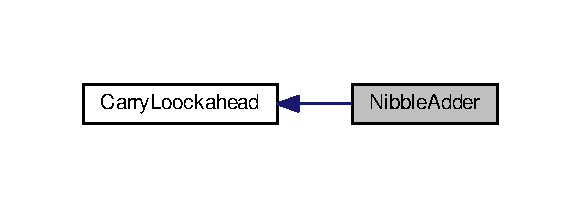
\includegraphics[width=279pt]{group___nibble_adder}
\end{center}
\end{figure}
\subsection*{Entities}
\begin{DoxyCompactItemize}
\item 
\hyperlink{classnibble__adder}{nibble\+\_\+adder} entity
\begin{DoxyCompactList}\small\item\em Addizionatore con carry-\/lookahead a quattro bit.

La cella somma tra loro due addendi ed un carry in ingresso; gli addendi sono espressi su quattro bit. Oltre a generare la somma, genera le funzioni \char`\"{}propagazione\char`\"{} e \char`\"{}generazione\char`\"{} del carry per eventuali blocchi \hyperlink{classnibble__adder}{nibble\+\_\+adder} posti a valle. \end{DoxyCompactList}\item 
\hyperlink{classnibble__adder_1_1structural}{structural} architecture
\begin{DoxyCompactList}\small\item\em Implementazione structural dell\textquotesingle{}entità \hyperlink{classnibble__adder}{nibble\+\_\+adder}.

Questa architettura istanzia una entità \hyperlink{classcla__carry__net}{cla\+\_\+carry\+\_\+net} ed una entità \hyperlink{classcla__adder__cell}{cla\+\_\+adder\+\_\+cell} per ogni bit su cui sono espressi gli addendi, connettendoli tra loro secondo lo schema riportato di seguito\+: . \end{DoxyCompactList}\end{DoxyCompactItemize}
\subsection*{Components}
 \begin{DoxyCompactItemize}
\item 
\hyperlink{group___nibble_adder_ga12bdc5892f526938e1447d663d152df8}{cla\+\_\+carry\+\_\+net}  {\bfseries }  
\item 
\hyperlink{group___nibble_adder_ga4f13eb52457f650b1d2cd352d9cacca9}{cla\+\_\+adder\+\_\+cell}  {\bfseries }  
\end{DoxyCompactItemize}
\subsection*{Ports}
 \begin{DoxyCompactItemize}
\item 
\hyperlink{group___nibble_adder_ga2c8945f4747b9a5448412c95fc281c87}{addendum1}  {\bfseries {\bfseries \textcolor{vhdlchar}{in}\textcolor{vhdlchar}{ }}} {\bfseries \textcolor{vhdlchar}{std\+\_\+logic\+\_\+vector}\textcolor{vhdlchar}{ }\textcolor{vhdlchar}{(}\textcolor{vhdlchar}{ }\textcolor{vhdlchar}{ } \textcolor{vhdldigit}{3} \textcolor{vhdlchar}{ }\textcolor{vhdlchar}{downto}\textcolor{vhdlchar}{ }\textcolor{vhdlchar}{ } \textcolor{vhdldigit}{0} \textcolor{vhdlchar}{ }\textcolor{vhdlchar}{)}\textcolor{vhdlchar}{ }} 
\begin{DoxyCompactList}\small\item\em addendo 1 \end{DoxyCompactList}\item 
\hyperlink{group___nibble_adder_gad1fa6d9d78208885ad2f4c417fc4b530}{addendum2}  {\bfseries {\bfseries \textcolor{vhdlchar}{in}\textcolor{vhdlchar}{ }}} {\bfseries \textcolor{vhdlchar}{std\+\_\+logic\+\_\+vector}\textcolor{vhdlchar}{ }\textcolor{vhdlchar}{(}\textcolor{vhdlchar}{ }\textcolor{vhdlchar}{ } \textcolor{vhdldigit}{3} \textcolor{vhdlchar}{ }\textcolor{vhdlchar}{downto}\textcolor{vhdlchar}{ }\textcolor{vhdlchar}{ } \textcolor{vhdldigit}{0} \textcolor{vhdlchar}{ }\textcolor{vhdlchar}{)}\textcolor{vhdlchar}{ }} 
\begin{DoxyCompactList}\small\item\em addendo 2 \end{DoxyCompactList}\item 
\hyperlink{group___nibble_adder_gaa556a73dc4a4de1a0d662b25adbcbe33}{carryin}  {\bfseries {\bfseries \textcolor{vhdlchar}{in}\textcolor{vhdlchar}{ }}} {\bfseries \textcolor{vhdlchar}{std\+\_\+logic}\textcolor{vhdlchar}{ }} 
\begin{DoxyCompactList}\small\item\em segnale di \char`\"{}carry-\/in\char`\"{}, prodotto da un eventuale \hyperlink{classnibble__adder}{nibble\+\_\+adder} a monte. \end{DoxyCompactList}\item 
\hyperlink{group___nibble_adder_ga422e8e7ee01fc7ac7b7390cd2ad8c87b}{propin}  {\bfseries {\bfseries \textcolor{vhdlchar}{in}\textcolor{vhdlchar}{ }}} {\bfseries \textcolor{vhdlchar}{std\+\_\+logic}\textcolor{vhdlchar}{ }} 
\begin{DoxyCompactList}\small\item\em funzione \char`\"{}propagazione\char`\"{}, prodotta da una eventuale \hyperlink{classnibble__adder}{nibble\+\_\+adder} a monte \end{DoxyCompactList}\item 
\hyperlink{group___nibble_adder_ga0a46d5193cb73eb993bc5d4f69741d0a}{genin}  {\bfseries {\bfseries \textcolor{vhdlchar}{in}\textcolor{vhdlchar}{ }}} {\bfseries \textcolor{vhdlchar}{std\+\_\+logic}\textcolor{vhdlchar}{ }} 
\begin{DoxyCompactList}\small\item\em funzione \char`\"{}generazione\char`\"{}, prodotta da una eventuale \hyperlink{classnibble__adder}{nibble\+\_\+adder} a monte \end{DoxyCompactList}\item 
\hyperlink{group___nibble_adder_ga5957c9cdd706cafd2da8855133a002c9}{propout}  {\bfseries {\bfseries \textcolor{vhdlchar}{out}\textcolor{vhdlchar}{ }}} {\bfseries \textcolor{vhdlchar}{std\+\_\+logic}\textcolor{vhdlchar}{ }} 
\item 
\hyperlink{group___nibble_adder_ga068cd5c4d23e284cb942702252ed1491}{genout}  {\bfseries {\bfseries \textcolor{vhdlchar}{out}\textcolor{vhdlchar}{ }}} {\bfseries \textcolor{vhdlchar}{std\+\_\+logic}\textcolor{vhdlchar}{ }} 
\item 
\hyperlink{group___nibble_adder_gadfe538323c3296159dd3b383325a996b}{sum}  {\bfseries {\bfseries \textcolor{vhdlchar}{out}\textcolor{vhdlchar}{ }}} {\bfseries \textcolor{vhdlchar}{std\+\_\+logic\+\_\+vector}\textcolor{vhdlchar}{ }\textcolor{vhdlchar}{(}\textcolor{vhdlchar}{ }\textcolor{vhdlchar}{ } \textcolor{vhdldigit}{3} \textcolor{vhdlchar}{ }\textcolor{vhdlchar}{downto}\textcolor{vhdlchar}{ }\textcolor{vhdlchar}{ } \textcolor{vhdldigit}{0} \textcolor{vhdlchar}{ }\textcolor{vhdlchar}{)}\textcolor{vhdlchar}{ }} 
\end{DoxyCompactItemize}
\subsection*{Signals}
 \begin{DoxyCompactItemize}
\item 
\hyperlink{group___nibble_adder_ga3abd8d433ff039baabc0c6fc2126578b}{prop} {\bfseries \textcolor{vhdlchar}{std\+\_\+logic\+\_\+vector}\textcolor{vhdlchar}{ }\textcolor{vhdlchar}{(}\textcolor{vhdlchar}{ }\textcolor{vhdlchar}{ } \textcolor{vhdldigit}{3} \textcolor{vhdlchar}{ }\textcolor{vhdlchar}{downto}\textcolor{vhdlchar}{ }\textcolor{vhdlchar}{ } \textcolor{vhdldigit}{0} \textcolor{vhdlchar}{ }\textcolor{vhdlchar}{)}\textcolor{vhdlchar}{ }} 
\item 
\hyperlink{group___nibble_adder_gac6c069fe4ec1c0a42272d3de4be6f45f}{gen} {\bfseries \textcolor{vhdlchar}{std\+\_\+logic\+\_\+vector}\textcolor{vhdlchar}{ }\textcolor{vhdlchar}{(}\textcolor{vhdlchar}{ }\textcolor{vhdlchar}{ } \textcolor{vhdldigit}{3} \textcolor{vhdlchar}{ }\textcolor{vhdlchar}{downto}\textcolor{vhdlchar}{ }\textcolor{vhdlchar}{ } \textcolor{vhdldigit}{0} \textcolor{vhdlchar}{ }\textcolor{vhdlchar}{)}\textcolor{vhdlchar}{ }} 
\item 
\hyperlink{group___nibble_adder_ga8f5524d80e551d479327a16bb32abcaa}{carry} {\bfseries \textcolor{vhdlchar}{std\+\_\+logic\+\_\+vector}\textcolor{vhdlchar}{ }\textcolor{vhdlchar}{(}\textcolor{vhdlchar}{ }\textcolor{vhdlchar}{ } \textcolor{vhdldigit}{3} \textcolor{vhdlchar}{ }\textcolor{vhdlchar}{downto}\textcolor{vhdlchar}{ }\textcolor{vhdlchar}{ } \textcolor{vhdldigit}{0} \textcolor{vhdlchar}{ }\textcolor{vhdlchar}{)}\textcolor{vhdlchar}{ }} 
\end{DoxyCompactItemize}


\subsection{Descrizione dettagliata}
Blocco elementare di somma a quattro bit. 



\subsection{Documentazione delle variabili}
\mbox{\Hypertarget{group___nibble_adder_ga2c8945f4747b9a5448412c95fc281c87}\label{group___nibble_adder_ga2c8945f4747b9a5448412c95fc281c87}} 
\index{Nibble\+Adder@{Nibble\+Adder}!addendum1@{addendum1}}
\index{addendum1@{addendum1}!Nibble\+Adder@{Nibble\+Adder}}
\subsubsection{\texorpdfstring{addendum1}{addendum1}}
{\footnotesize\ttfamily \hyperlink{group___nibble_adder_ga2c8945f4747b9a5448412c95fc281c87}{addendum1} {\bfseries \textcolor{vhdlchar}{in}\textcolor{vhdlchar}{ }} {\bfseries \textcolor{vhdlchar}{std\+\_\+logic\+\_\+vector}\textcolor{vhdlchar}{ }\textcolor{vhdlchar}{(}\textcolor{vhdlchar}{ }\textcolor{vhdlchar}{ } \textcolor{vhdldigit}{3} \textcolor{vhdlchar}{ }\textcolor{vhdlchar}{downto}\textcolor{vhdlchar}{ }\textcolor{vhdlchar}{ } \textcolor{vhdldigit}{0} \textcolor{vhdlchar}{ }\textcolor{vhdlchar}{)}\textcolor{vhdlchar}{ }} \hspace{0.3cm}{\ttfamily [Port]}}



addendo 1 

\mbox{\Hypertarget{group___nibble_adder_gad1fa6d9d78208885ad2f4c417fc4b530}\label{group___nibble_adder_gad1fa6d9d78208885ad2f4c417fc4b530}} 
\index{Nibble\+Adder@{Nibble\+Adder}!addendum2@{addendum2}}
\index{addendum2@{addendum2}!Nibble\+Adder@{Nibble\+Adder}}
\subsubsection{\texorpdfstring{addendum2}{addendum2}}
{\footnotesize\ttfamily \hyperlink{group___nibble_adder_gad1fa6d9d78208885ad2f4c417fc4b530}{addendum2} {\bfseries \textcolor{vhdlchar}{in}\textcolor{vhdlchar}{ }} {\bfseries \textcolor{vhdlchar}{std\+\_\+logic\+\_\+vector}\textcolor{vhdlchar}{ }\textcolor{vhdlchar}{(}\textcolor{vhdlchar}{ }\textcolor{vhdlchar}{ } \textcolor{vhdldigit}{3} \textcolor{vhdlchar}{ }\textcolor{vhdlchar}{downto}\textcolor{vhdlchar}{ }\textcolor{vhdlchar}{ } \textcolor{vhdldigit}{0} \textcolor{vhdlchar}{ }\textcolor{vhdlchar}{)}\textcolor{vhdlchar}{ }} \hspace{0.3cm}{\ttfamily [Port]}}



addendo 2 

\mbox{\Hypertarget{group___nibble_adder_ga8f5524d80e551d479327a16bb32abcaa}\label{group___nibble_adder_ga8f5524d80e551d479327a16bb32abcaa}} 
\index{Nibble\+Adder@{Nibble\+Adder}!carry@{carry}}
\index{carry@{carry}!Nibble\+Adder@{Nibble\+Adder}}
\subsubsection{\texorpdfstring{carry}{carry}}
{\footnotesize\ttfamily \hyperlink{group___nibble_adder_ga8f5524d80e551d479327a16bb32abcaa}{carry} {\bfseries \textcolor{vhdlchar}{std\+\_\+logic\+\_\+vector}\textcolor{vhdlchar}{ }\textcolor{vhdlchar}{(}\textcolor{vhdlchar}{ }\textcolor{vhdlchar}{ } \textcolor{vhdldigit}{3} \textcolor{vhdlchar}{ }\textcolor{vhdlchar}{downto}\textcolor{vhdlchar}{ }\textcolor{vhdlchar}{ } \textcolor{vhdldigit}{0} \textcolor{vhdlchar}{ }\textcolor{vhdlchar}{)}\textcolor{vhdlchar}{ }} \hspace{0.3cm}{\ttfamily [Signal]}}

funzione \char`\"{}generazione\char`\"{} prodotta da \hyperlink{classcla__adder__cell}{cla\+\_\+adder\+\_\+cell}; vale 1 quando, sulla base degli ingressi, un adder generera\textquotesingle{} un carry in uscita; gen(i) = add(i) A\+ND add(i); in questo caso viene prodotta da quattro blocchi \hyperlink{classcla__adder__cell}{cla\+\_\+adder\+\_\+cell} sulla base dei loro ingressi \mbox{\Hypertarget{group___nibble_adder_gaa556a73dc4a4de1a0d662b25adbcbe33}\label{group___nibble_adder_gaa556a73dc4a4de1a0d662b25adbcbe33}} 
\index{Nibble\+Adder@{Nibble\+Adder}!carryin@{carryin}}
\index{carryin@{carryin}!Nibble\+Adder@{Nibble\+Adder}}
\subsubsection{\texorpdfstring{carryin}{carryin}}
{\footnotesize\ttfamily \hyperlink{group___nibble_adder_gaa556a73dc4a4de1a0d662b25adbcbe33}{carryin} {\bfseries \textcolor{vhdlchar}{in}\textcolor{vhdlchar}{ }} {\bfseries \textcolor{vhdlchar}{std\+\_\+logic}\textcolor{vhdlchar}{ }} \hspace{0.3cm}{\ttfamily [Port]}}



segnale di \char`\"{}carry-\/in\char`\"{}, prodotto da un eventuale \hyperlink{classnibble__adder}{nibble\+\_\+adder} a monte. 

\mbox{\Hypertarget{group___nibble_adder_ga4f13eb52457f650b1d2cd352d9cacca9}\label{group___nibble_adder_ga4f13eb52457f650b1d2cd352d9cacca9}} 
\index{Nibble\+Adder@{Nibble\+Adder}!cla\+\_\+adder\+\_\+cell@{cla\+\_\+adder\+\_\+cell}}
\index{cla\+\_\+adder\+\_\+cell@{cla\+\_\+adder\+\_\+cell}!Nibble\+Adder@{Nibble\+Adder}}
\subsubsection{\texorpdfstring{cla\+\_\+adder\+\_\+cell}{cla\_adder\_cell}}
{\footnotesize\ttfamily \hyperlink{group___nibble_adder_ga4f13eb52457f650b1d2cd352d9cacca9}{cla\+\_\+adder\+\_\+cell} {\bfseries \textcolor{vhdlchar}{ }} \hspace{0.3cm}{\ttfamily [Component]}}

\mbox{\Hypertarget{group___nibble_adder_ga12bdc5892f526938e1447d663d152df8}\label{group___nibble_adder_ga12bdc5892f526938e1447d663d152df8}} 
\index{Nibble\+Adder@{Nibble\+Adder}!cla\+\_\+carry\+\_\+net@{cla\+\_\+carry\+\_\+net}}
\index{cla\+\_\+carry\+\_\+net@{cla\+\_\+carry\+\_\+net}!Nibble\+Adder@{Nibble\+Adder}}
\subsubsection{\texorpdfstring{cla\+\_\+carry\+\_\+net}{cla\_carry\_net}}
{\footnotesize\ttfamily \hyperlink{group___nibble_adder_ga12bdc5892f526938e1447d663d152df8}{cla\+\_\+carry\+\_\+net} {\bfseries \textcolor{vhdlchar}{ }} \hspace{0.3cm}{\ttfamily [Component]}}

\mbox{\Hypertarget{group___nibble_adder_gac6c069fe4ec1c0a42272d3de4be6f45f}\label{group___nibble_adder_gac6c069fe4ec1c0a42272d3de4be6f45f}} 
\index{Nibble\+Adder@{Nibble\+Adder}!gen@{gen}}
\index{gen@{gen}!Nibble\+Adder@{Nibble\+Adder}}
\subsubsection{\texorpdfstring{gen}{gen}}
{\footnotesize\ttfamily \hyperlink{group___nibble_adder_gac6c069fe4ec1c0a42272d3de4be6f45f}{gen} {\bfseries \textcolor{vhdlchar}{std\+\_\+logic\+\_\+vector}\textcolor{vhdlchar}{ }\textcolor{vhdlchar}{(}\textcolor{vhdlchar}{ }\textcolor{vhdlchar}{ } \textcolor{vhdldigit}{3} \textcolor{vhdlchar}{ }\textcolor{vhdlchar}{downto}\textcolor{vhdlchar}{ }\textcolor{vhdlchar}{ } \textcolor{vhdldigit}{0} \textcolor{vhdlchar}{ }\textcolor{vhdlchar}{)}\textcolor{vhdlchar}{ }} \hspace{0.3cm}{\ttfamily [Signal]}}

funzione “propagazione” prodotta da \hyperlink{classcla__adder__cell}{cla\+\_\+adder\+\_\+cell}; vale 1 quando, sulla base degli ingressi, un adder propaghera\textquotesingle{} un eventuale carry in ingresso; prop(i) = add(i) OR add(i); in questo caso viene prodotta da quattro blocchi \hyperlink{classcla__adder__cell}{cla\+\_\+adder\+\_\+cell} sulla base dei loro ingressi \mbox{\Hypertarget{group___nibble_adder_ga0a46d5193cb73eb993bc5d4f69741d0a}\label{group___nibble_adder_ga0a46d5193cb73eb993bc5d4f69741d0a}} 
\index{Nibble\+Adder@{Nibble\+Adder}!genin@{genin}}
\index{genin@{genin}!Nibble\+Adder@{Nibble\+Adder}}
\subsubsection{\texorpdfstring{genin}{genin}}
{\footnotesize\ttfamily \hyperlink{group___nibble_adder_ga0a46d5193cb73eb993bc5d4f69741d0a}{genin} {\bfseries \textcolor{vhdlchar}{in}\textcolor{vhdlchar}{ }} {\bfseries \textcolor{vhdlchar}{std\+\_\+logic}\textcolor{vhdlchar}{ }} \hspace{0.3cm}{\ttfamily [Port]}}



funzione \char`\"{}generazione\char`\"{}, prodotta da una eventuale \hyperlink{classnibble__adder}{nibble\+\_\+adder} a monte 

\mbox{\Hypertarget{group___nibble_adder_ga068cd5c4d23e284cb942702252ed1491}\label{group___nibble_adder_ga068cd5c4d23e284cb942702252ed1491}} 
\index{Nibble\+Adder@{Nibble\+Adder}!genout@{genout}}
\index{genout@{genout}!Nibble\+Adder@{Nibble\+Adder}}
\subsubsection{\texorpdfstring{genout}{genout}}
{\footnotesize\ttfamily \hyperlink{group___nibble_adder_ga068cd5c4d23e284cb942702252ed1491}{genout} {\bfseries \textcolor{vhdlchar}{out}\textcolor{vhdlchar}{ }} {\bfseries \textcolor{vhdlchar}{std\+\_\+logic}\textcolor{vhdlchar}{ }} \hspace{0.3cm}{\ttfamily [Port]}}

funzione \char`\"{}propagazione\char`\"{} da porre in ingresso ad un eventuale blocco \hyperlink{classnibble__adder}{nibble\+\_\+adder} a valle \mbox{\Hypertarget{group___nibble_adder_ga3abd8d433ff039baabc0c6fc2126578b}\label{group___nibble_adder_ga3abd8d433ff039baabc0c6fc2126578b}} 
\index{Nibble\+Adder@{Nibble\+Adder}!prop@{prop}}
\index{prop@{prop}!Nibble\+Adder@{Nibble\+Adder}}
\subsubsection{\texorpdfstring{prop}{prop}}
{\footnotesize\ttfamily \hyperlink{group___nibble_adder_ga3abd8d433ff039baabc0c6fc2126578b}{prop} {\bfseries \textcolor{vhdlchar}{std\+\_\+logic\+\_\+vector}\textcolor{vhdlchar}{ }\textcolor{vhdlchar}{(}\textcolor{vhdlchar}{ }\textcolor{vhdlchar}{ } \textcolor{vhdldigit}{3} \textcolor{vhdlchar}{ }\textcolor{vhdlchar}{downto}\textcolor{vhdlchar}{ }\textcolor{vhdlchar}{ } \textcolor{vhdldigit}{0} \textcolor{vhdlchar}{ }\textcolor{vhdlchar}{)}\textcolor{vhdlchar}{ }} \hspace{0.3cm}{\ttfamily [Signal]}}

\mbox{\Hypertarget{group___nibble_adder_ga422e8e7ee01fc7ac7b7390cd2ad8c87b}\label{group___nibble_adder_ga422e8e7ee01fc7ac7b7390cd2ad8c87b}} 
\index{Nibble\+Adder@{Nibble\+Adder}!propin@{propin}}
\index{propin@{propin}!Nibble\+Adder@{Nibble\+Adder}}
\subsubsection{\texorpdfstring{propin}{propin}}
{\footnotesize\ttfamily \hyperlink{group___nibble_adder_ga422e8e7ee01fc7ac7b7390cd2ad8c87b}{propin} {\bfseries \textcolor{vhdlchar}{in}\textcolor{vhdlchar}{ }} {\bfseries \textcolor{vhdlchar}{std\+\_\+logic}\textcolor{vhdlchar}{ }} \hspace{0.3cm}{\ttfamily [Port]}}



funzione \char`\"{}propagazione\char`\"{}, prodotta da una eventuale \hyperlink{classnibble__adder}{nibble\+\_\+adder} a monte 

\mbox{\Hypertarget{group___nibble_adder_ga5957c9cdd706cafd2da8855133a002c9}\label{group___nibble_adder_ga5957c9cdd706cafd2da8855133a002c9}} 
\index{Nibble\+Adder@{Nibble\+Adder}!propout@{propout}}
\index{propout@{propout}!Nibble\+Adder@{Nibble\+Adder}}
\subsubsection{\texorpdfstring{propout}{propout}}
{\footnotesize\ttfamily \hyperlink{group___nibble_adder_ga5957c9cdd706cafd2da8855133a002c9}{propout} {\bfseries \textcolor{vhdlchar}{out}\textcolor{vhdlchar}{ }} {\bfseries \textcolor{vhdlchar}{std\+\_\+logic}\textcolor{vhdlchar}{ }} \hspace{0.3cm}{\ttfamily [Port]}}

\mbox{\Hypertarget{group___nibble_adder_gadfe538323c3296159dd3b383325a996b}\label{group___nibble_adder_gadfe538323c3296159dd3b383325a996b}} 
\index{Nibble\+Adder@{Nibble\+Adder}!sum@{sum}}
\index{sum@{sum}!Nibble\+Adder@{Nibble\+Adder}}
\subsubsection{\texorpdfstring{sum}{sum}}
{\footnotesize\ttfamily \hyperlink{group___nibble_adder_gadfe538323c3296159dd3b383325a996b}{sum} {\bfseries \textcolor{vhdlchar}{out}\textcolor{vhdlchar}{ }} {\bfseries \textcolor{vhdlchar}{std\+\_\+logic\+\_\+vector}\textcolor{vhdlchar}{ }\textcolor{vhdlchar}{(}\textcolor{vhdlchar}{ }\textcolor{vhdlchar}{ } \textcolor{vhdldigit}{3} \textcolor{vhdlchar}{ }\textcolor{vhdlchar}{downto}\textcolor{vhdlchar}{ }\textcolor{vhdlchar}{ } \textcolor{vhdldigit}{0} \textcolor{vhdlchar}{ }\textcolor{vhdlchar}{)}\textcolor{vhdlchar}{ }} \hspace{0.3cm}{\ttfamily [Port]}}

funzione \char`\"{}generazione\char`\"{} da porre in ingresso ad un eventuale blocco \hyperlink{classnibble__adder}{nibble\+\_\+adder} a valle 
\chapter{Documentazione delle classi}
\hypertarget{classadder}{}\section{adder Entity Reference}
\label{classadder}\index{adder@{adder}}


Diagramma delle classi per adder
\nopagebreak
\begin{figure}[H]
\begin{center}
\leavevmode
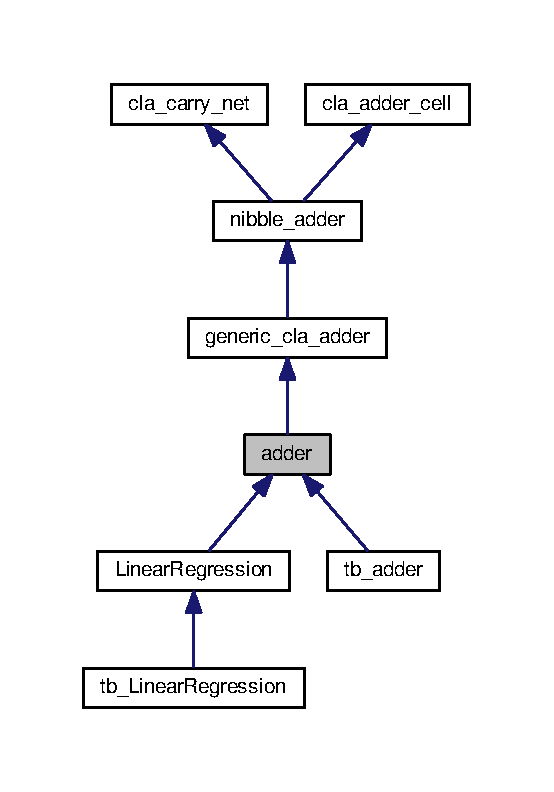
\includegraphics[width=259pt]{classadder__inherit__graph}
\end{center}
\end{figure}


Diagramma di collaborazione per adder\+:\nopagebreak
\begin{figure}[H]
\begin{center}
\leavevmode
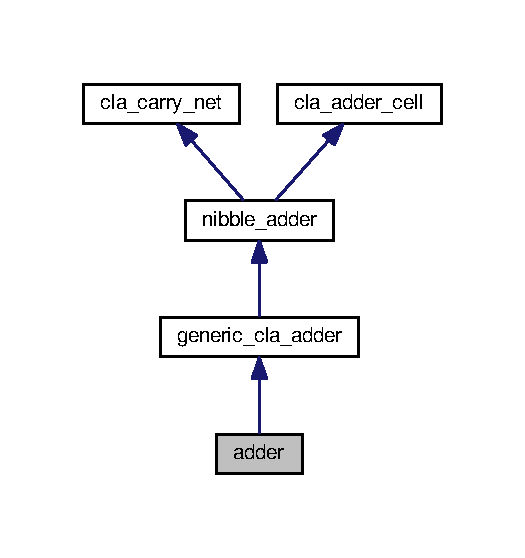
\includegraphics[width=252pt]{classadder__coll__graph}
\end{center}
\end{figure}
\subsection*{Entities}
\begin{DoxyCompactItemize}
\item 
\hyperlink{classadder_1_1structural}{structural} architecture
\begin{DoxyCompactList}\small\item\em Implementazione mista structural per l\textquotesingle{}entity adder.

A seconda del valore del parametro use\+\_\+custom, verrà istanziato
\begin{DoxyItemize}
\item un sommatore full-\/custom \hyperlink{classgeneric__cla__adder}{generic\+\_\+cla\+\_\+adder}, se use\+\_\+custom = true;
\item un sommatore la cui implementazione è stabilita dal sintetizzatore, se use\+\_\+custom = false; Nel caso in cui venga istanziato il sommatore custom, è richiesto che il numero di bit con il quale sono espressi gli addendi, e di conseguenza quello in vui verrà espressa la loro somma, sia multiplo di quattro. 
\end{DoxyItemize}\end{DoxyCompactList}\end{DoxyCompactItemize}
\subsection*{Generics}
 \begin{DoxyCompactItemize}
\item 
\hyperlink{group___adder_gae1435c07d0cd54b521535e2f8de6f94e}{nbits} {\bfseries {\bfseries \textcolor{vhdlchar}{natural}\textcolor{vhdlchar}{ }\textcolor{vhdlchar}{ }\textcolor{vhdlchar}{\+:}\textcolor{vhdlchar}{=}\textcolor{vhdlchar}{ }\textcolor{vhdlchar}{ } \textcolor{vhdldigit}{32} \textcolor{vhdlchar}{ }}}
\item 
\hyperlink{group___adder_gadf05ca347ec6d3c85740dc697469b3db}{use\+\_\+custom} {\bfseries {\bfseries \textcolor{vhdlchar}{boolean}\textcolor{vhdlchar}{ }\textcolor{vhdlchar}{ }\textcolor{vhdlchar}{\+:}\textcolor{vhdlchar}{=}\textcolor{vhdlchar}{ }\textcolor{vhdlchar}{ }\textcolor{vhdlchar}{ }\textcolor{vhdlchar}{ }\textcolor{vhdlchar}{false}\textcolor{vhdlchar}{ }}}
\end{DoxyCompactItemize}
\subsection*{Ports}
 \begin{DoxyCompactItemize}
\item 
\hyperlink{group___adder_gad6ed6073f8ded668a403a0f7d85c53e8}{add1}  {\bfseries {\bfseries \textcolor{vhdlchar}{in}\textcolor{vhdlchar}{ }}} {\bfseries \textcolor{vhdlchar}{std\+\_\+logic\+\_\+vector}\textcolor{vhdlchar}{ }\textcolor{vhdlchar}{(}\textcolor{vhdlchar}{ }\textcolor{vhdlchar}{ }\textcolor{vhdlchar}{ }\textcolor{vhdlchar}{ }{\bfseries \hyperlink{group___adder_gae1435c07d0cd54b521535e2f8de6f94e}{nbits}} \textcolor{vhdlchar}{-\/}\textcolor{vhdlchar}{ } \textcolor{vhdldigit}{1} \textcolor{vhdlchar}{ }\textcolor{vhdlchar}{downto}\textcolor{vhdlchar}{ }\textcolor{vhdlchar}{ } \textcolor{vhdldigit}{0} \textcolor{vhdlchar}{ }\textcolor{vhdlchar}{)}\textcolor{vhdlchar}{ }} 
\begin{DoxyCompactList}\small\item\em addendo 1 \end{DoxyCompactList}\item 
\hyperlink{group___adder_gabf87ad241134c4d313c708910677575e}{add2}  {\bfseries {\bfseries \textcolor{vhdlchar}{in}\textcolor{vhdlchar}{ }}} {\bfseries \textcolor{vhdlchar}{std\+\_\+logic\+\_\+vector}\textcolor{vhdlchar}{ }\textcolor{vhdlchar}{(}\textcolor{vhdlchar}{ }\textcolor{vhdlchar}{ }\textcolor{vhdlchar}{ }\textcolor{vhdlchar}{ }{\bfseries \hyperlink{group___adder_gae1435c07d0cd54b521535e2f8de6f94e}{nbits}} \textcolor{vhdlchar}{-\/}\textcolor{vhdlchar}{ } \textcolor{vhdldigit}{1} \textcolor{vhdlchar}{ }\textcolor{vhdlchar}{downto}\textcolor{vhdlchar}{ }\textcolor{vhdlchar}{ } \textcolor{vhdldigit}{0} \textcolor{vhdlchar}{ }\textcolor{vhdlchar}{)}\textcolor{vhdlchar}{ }} 
\begin{DoxyCompactList}\small\item\em addendo 2 \end{DoxyCompactList}\item 
\hyperlink{group___adder_ga01f6ea3ddb4d1519676217bcb5959de8}{sum}  {\bfseries {\bfseries \textcolor{vhdlchar}{out}\textcolor{vhdlchar}{ }}} {\bfseries \textcolor{vhdlchar}{std\+\_\+logic\+\_\+vector}\textcolor{vhdlchar}{ }\textcolor{vhdlchar}{(}\textcolor{vhdlchar}{ }\textcolor{vhdlchar}{ }\textcolor{vhdlchar}{ }\textcolor{vhdlchar}{ }{\bfseries \hyperlink{group___adder_gae1435c07d0cd54b521535e2f8de6f94e}{nbits}} \textcolor{vhdlchar}{-\/}\textcolor{vhdlchar}{ } \textcolor{vhdldigit}{1} \textcolor{vhdlchar}{ }\textcolor{vhdlchar}{downto}\textcolor{vhdlchar}{ }\textcolor{vhdlchar}{ } \textcolor{vhdldigit}{0} \textcolor{vhdlchar}{ }\textcolor{vhdlchar}{)}\textcolor{vhdlchar}{ }} 
\begin{DoxyCompactList}\small\item\em somma degli addendi \end{DoxyCompactList}\item 
\hyperlink{group___adder_ga9650307dde287e0bcfa1e26370c006c2}{overflow}  {\bfseries {\bfseries \textcolor{vhdlchar}{out}\textcolor{vhdlchar}{ }}} {\bfseries \textcolor{vhdlchar}{std\+\_\+logic}\textcolor{vhdlchar}{ }} 
\end{DoxyCompactItemize}


\subsection{Descrizione dettagliata}
Sommatore a due addendi.

Il sommatore permette di effettuare una somma di due addendi espressi su un certo numero di bit. La somma dei due addendi viene espressa sullo stesso numero di bit. Quando il risultato prodotto dalla somma degli addendi non è correttamente rappresentato su tale numero di bit, un flag indica la condizione di overflow. 

La documentazione per questa classe è stata generata a partire dal seguente file\+:\begin{DoxyCompactItemize}
\item 
Src/adder/\hyperlink{adder_8vhd}{adder.\+vhd}\end{DoxyCompactItemize}

\hypertarget{classtb__adder_1_1behavior}{}\section{behavior Architecture Reference}
\label{classtb__adder_1_1behavior}\index{behavior@{behavior}}
\subsection*{Processes}
 \begin{DoxyCompactItemize}
\item 
\hyperlink{classtb__adder_1_1behavior_ad2efa6785cff833c341e27596b21aeb5}{stim\+\_\+proc}{\bfseries  (  )}
\end{DoxyCompactItemize}
\subsection*{Components}
 \begin{DoxyCompactItemize}
\item 
\hyperlink{classtb__adder_1_1behavior_a9d7a8a381439c61aea549e7a47ec7a6f}{adder}  {\bfseries }  
\end{DoxyCompactItemize}
\subsection*{Constants}
 \begin{DoxyCompactItemize}
\item 
\hyperlink{classtb__adder_1_1behavior_aff8823a253db156c5a7a40d1b813343f}{nbits} {\bfseries \textcolor{vhdlchar}{natural}\textcolor{vhdlchar}{ }\textcolor{vhdlchar}{ }\textcolor{vhdlchar}{\+:}\textcolor{vhdlchar}{=}\textcolor{vhdlchar}{ }\textcolor{vhdlchar}{ } \textcolor{vhdldigit}{12} \textcolor{vhdlchar}{ }} 
\item 
\hyperlink{classtb__adder_1_1behavior_ae53b6cfbb1b5d32c932c417636d6ac3c}{use\+\_\+custom} {\bfseries \textcolor{vhdlchar}{boolean}\textcolor{vhdlchar}{ }\textcolor{vhdlchar}{ }\textcolor{vhdlchar}{\+:}\textcolor{vhdlchar}{=}\textcolor{vhdlchar}{ }\textcolor{vhdlchar}{ }\textcolor{vhdlchar}{ }\textcolor{vhdlchar}{ }\textcolor{vhdlchar}{true}\textcolor{vhdlchar}{ }} 
\end{DoxyCompactItemize}
\subsection*{Signals}
 \begin{DoxyCompactItemize}
\item 
\hyperlink{classtb__adder_1_1behavior_a1c7a41b72844f6ed4f7cf1ab81102a2a}{add1} {\bfseries \textcolor{vhdlchar}{std\+\_\+logic\+\_\+vector}\textcolor{vhdlchar}{ }\textcolor{vhdlchar}{(}\textcolor{vhdlchar}{ }\textcolor{vhdlchar}{ }\textcolor{vhdlchar}{ }\textcolor{vhdlchar}{ }{\bfseries \hyperlink{classtb__adder_1_1behavior_aff8823a253db156c5a7a40d1b813343f}{nbits}} \textcolor{vhdlchar}{-\/}\textcolor{vhdlchar}{ } \textcolor{vhdldigit}{1} \textcolor{vhdlchar}{ }\textcolor{vhdlchar}{downto}\textcolor{vhdlchar}{ }\textcolor{vhdlchar}{ } \textcolor{vhdldigit}{0} \textcolor{vhdlchar}{ }\textcolor{vhdlchar}{)}\textcolor{vhdlchar}{ }\textcolor{vhdlchar}{ }\textcolor{vhdlchar}{ }\textcolor{vhdlchar}{\+:}\textcolor{vhdlchar}{=}\textcolor{vhdlchar}{ }\textcolor{vhdlchar}{(}\textcolor{vhdlchar}{ }\textcolor{vhdlchar}{ }\textcolor{vhdlchar}{others}\textcolor{vhdlchar}{ }\textcolor{vhdlchar}{ }\textcolor{vhdlchar}{=}\textcolor{vhdlchar}{ }\textcolor{vhdlchar}{$>$}\textcolor{vhdlchar}{ }\textcolor{vhdlchar}{\textquotesingle{}}\textcolor{vhdlchar}{ } \textcolor{vhdldigit}{0} \textcolor{vhdlchar}{ }\textcolor{vhdlchar}{\textquotesingle{}}\textcolor{vhdlchar}{ }\textcolor{vhdlchar}{)}\textcolor{vhdlchar}{ }} 
\item 
\hyperlink{classtb__adder_1_1behavior_aa713d21db1284f6652f7e63e60cacaa1}{add2} {\bfseries \textcolor{vhdlchar}{std\+\_\+logic\+\_\+vector}\textcolor{vhdlchar}{ }\textcolor{vhdlchar}{(}\textcolor{vhdlchar}{ }\textcolor{vhdlchar}{ }\textcolor{vhdlchar}{ }\textcolor{vhdlchar}{ }{\bfseries \hyperlink{classtb__adder_1_1behavior_aff8823a253db156c5a7a40d1b813343f}{nbits}} \textcolor{vhdlchar}{-\/}\textcolor{vhdlchar}{ } \textcolor{vhdldigit}{1} \textcolor{vhdlchar}{ }\textcolor{vhdlchar}{downto}\textcolor{vhdlchar}{ }\textcolor{vhdlchar}{ } \textcolor{vhdldigit}{0} \textcolor{vhdlchar}{ }\textcolor{vhdlchar}{)}\textcolor{vhdlchar}{ }\textcolor{vhdlchar}{ }\textcolor{vhdlchar}{ }\textcolor{vhdlchar}{\+:}\textcolor{vhdlchar}{=}\textcolor{vhdlchar}{ }\textcolor{vhdlchar}{(}\textcolor{vhdlchar}{ }\textcolor{vhdlchar}{ }\textcolor{vhdlchar}{others}\textcolor{vhdlchar}{ }\textcolor{vhdlchar}{ }\textcolor{vhdlchar}{=}\textcolor{vhdlchar}{ }\textcolor{vhdlchar}{$>$}\textcolor{vhdlchar}{ }\textcolor{vhdlchar}{\textquotesingle{}}\textcolor{vhdlchar}{ } \textcolor{vhdldigit}{0} \textcolor{vhdlchar}{ }\textcolor{vhdlchar}{\textquotesingle{}}\textcolor{vhdlchar}{ }\textcolor{vhdlchar}{)}\textcolor{vhdlchar}{ }} 
\item 
\hyperlink{classtb__adder_1_1behavior_a5db139547621616405be3e820278d444}{sum} {\bfseries \textcolor{vhdlchar}{std\+\_\+logic\+\_\+vector}\textcolor{vhdlchar}{ }\textcolor{vhdlchar}{(}\textcolor{vhdlchar}{ }\textcolor{vhdlchar}{ }\textcolor{vhdlchar}{ }\textcolor{vhdlchar}{ }{\bfseries \hyperlink{classtb__adder_1_1behavior_aff8823a253db156c5a7a40d1b813343f}{nbits}} \textcolor{vhdlchar}{-\/}\textcolor{vhdlchar}{ } \textcolor{vhdldigit}{1} \textcolor{vhdlchar}{ }\textcolor{vhdlchar}{downto}\textcolor{vhdlchar}{ }\textcolor{vhdlchar}{ } \textcolor{vhdldigit}{0} \textcolor{vhdlchar}{ }\textcolor{vhdlchar}{)}\textcolor{vhdlchar}{ }\textcolor{vhdlchar}{ }\textcolor{vhdlchar}{ }\textcolor{vhdlchar}{\+:}\textcolor{vhdlchar}{=}\textcolor{vhdlchar}{ }\textcolor{vhdlchar}{(}\textcolor{vhdlchar}{ }\textcolor{vhdlchar}{ }\textcolor{vhdlchar}{others}\textcolor{vhdlchar}{ }\textcolor{vhdlchar}{ }\textcolor{vhdlchar}{=}\textcolor{vhdlchar}{ }\textcolor{vhdlchar}{$>$}\textcolor{vhdlchar}{ }\textcolor{vhdlchar}{\textquotesingle{}}\textcolor{vhdlchar}{ } \textcolor{vhdldigit}{0} \textcolor{vhdlchar}{ }\textcolor{vhdlchar}{\textquotesingle{}}\textcolor{vhdlchar}{ }\textcolor{vhdlchar}{)}\textcolor{vhdlchar}{ }} 
\item 
\hyperlink{classtb__adder_1_1behavior_ab579763af0d4bea3c24be9431798eeea}{overflow} {\bfseries \textcolor{vhdlchar}{std\+\_\+logic}\textcolor{vhdlchar}{ }\textcolor{vhdlchar}{ }\textcolor{vhdlchar}{\+:}\textcolor{vhdlchar}{=}\textcolor{vhdlchar}{ }\textcolor{vhdlchar}{ }\textcolor{vhdlchar}{\textquotesingle{}}\textcolor{vhdlchar}{ } \textcolor{vhdldigit}{0} \textcolor{vhdlchar}{ }\textcolor{vhdlchar}{\textquotesingle{}}\textcolor{vhdlchar}{ }} 
\end{DoxyCompactItemize}
\subsection*{Instantiations}
 \begin{DoxyCompactItemize}
\item 
\hyperlink{classtb__adder_1_1behavior_a1619316ad715601eb5d3559db829ac05}{uut}  {\bfseries adder}   
\end{DoxyCompactItemize}


\subsection{Documentazione delle funzioni membro}
\mbox{\Hypertarget{classtb__adder_1_1behavior_ad2efa6785cff833c341e27596b21aeb5}\label{classtb__adder_1_1behavior_ad2efa6785cff833c341e27596b21aeb5}} 
\index{tb\+\_\+adder\+::behavior@{tb\+\_\+adder\+::behavior}!stim\+\_\+proc@{stim\+\_\+proc}}
\index{stim\+\_\+proc@{stim\+\_\+proc}!tb\+\_\+adder\+::behavior@{tb\+\_\+adder\+::behavior}}
\subsubsection{\texorpdfstring{stim\+\_\+proc()}{stim\_proc()}}
{\footnotesize\ttfamily stim\+\_\+proc (\begin{DoxyParamCaption}{ }\end{DoxyParamCaption})}



\subsection{Documentazione dei membri dato}
\mbox{\Hypertarget{classtb__adder_1_1behavior_a1c7a41b72844f6ed4f7cf1ab81102a2a}\label{classtb__adder_1_1behavior_a1c7a41b72844f6ed4f7cf1ab81102a2a}} 
\index{tb\+\_\+adder\+::behavior@{tb\+\_\+adder\+::behavior}!add1@{add1}}
\index{add1@{add1}!tb\+\_\+adder\+::behavior@{tb\+\_\+adder\+::behavior}}
\subsubsection{\texorpdfstring{add1}{add1}}
{\footnotesize\ttfamily \hyperlink{classtb__adder_1_1behavior_a1c7a41b72844f6ed4f7cf1ab81102a2a}{add1} {\bfseries \textcolor{vhdlchar}{std\+\_\+logic\+\_\+vector}\textcolor{vhdlchar}{ }\textcolor{vhdlchar}{(}\textcolor{vhdlchar}{ }\textcolor{vhdlchar}{ }\textcolor{vhdlchar}{ }\textcolor{vhdlchar}{ }{\bfseries \hyperlink{classtb__adder_1_1behavior_aff8823a253db156c5a7a40d1b813343f}{nbits}} \textcolor{vhdlchar}{-\/}\textcolor{vhdlchar}{ } \textcolor{vhdldigit}{1} \textcolor{vhdlchar}{ }\textcolor{vhdlchar}{downto}\textcolor{vhdlchar}{ }\textcolor{vhdlchar}{ } \textcolor{vhdldigit}{0} \textcolor{vhdlchar}{ }\textcolor{vhdlchar}{)}\textcolor{vhdlchar}{ }\textcolor{vhdlchar}{ }\textcolor{vhdlchar}{ }\textcolor{vhdlchar}{\+:}\textcolor{vhdlchar}{=}\textcolor{vhdlchar}{ }\textcolor{vhdlchar}{(}\textcolor{vhdlchar}{ }\textcolor{vhdlchar}{ }\textcolor{vhdlchar}{others}\textcolor{vhdlchar}{ }\textcolor{vhdlchar}{ }\textcolor{vhdlchar}{=}\textcolor{vhdlchar}{ }\textcolor{vhdlchar}{$>$}\textcolor{vhdlchar}{ }\textcolor{vhdlchar}{\textquotesingle{}}\textcolor{vhdlchar}{ } \textcolor{vhdldigit}{0} \textcolor{vhdlchar}{ }\textcolor{vhdlchar}{\textquotesingle{}}\textcolor{vhdlchar}{ }\textcolor{vhdlchar}{)}\textcolor{vhdlchar}{ }} \hspace{0.3cm}{\ttfamily [Signal]}}

\mbox{\Hypertarget{classtb__adder_1_1behavior_aa713d21db1284f6652f7e63e60cacaa1}\label{classtb__adder_1_1behavior_aa713d21db1284f6652f7e63e60cacaa1}} 
\index{tb\+\_\+adder\+::behavior@{tb\+\_\+adder\+::behavior}!add2@{add2}}
\index{add2@{add2}!tb\+\_\+adder\+::behavior@{tb\+\_\+adder\+::behavior}}
\subsubsection{\texorpdfstring{add2}{add2}}
{\footnotesize\ttfamily \hyperlink{classtb__adder_1_1behavior_aa713d21db1284f6652f7e63e60cacaa1}{add2} {\bfseries \textcolor{vhdlchar}{std\+\_\+logic\+\_\+vector}\textcolor{vhdlchar}{ }\textcolor{vhdlchar}{(}\textcolor{vhdlchar}{ }\textcolor{vhdlchar}{ }\textcolor{vhdlchar}{ }\textcolor{vhdlchar}{ }{\bfseries \hyperlink{classtb__adder_1_1behavior_aff8823a253db156c5a7a40d1b813343f}{nbits}} \textcolor{vhdlchar}{-\/}\textcolor{vhdlchar}{ } \textcolor{vhdldigit}{1} \textcolor{vhdlchar}{ }\textcolor{vhdlchar}{downto}\textcolor{vhdlchar}{ }\textcolor{vhdlchar}{ } \textcolor{vhdldigit}{0} \textcolor{vhdlchar}{ }\textcolor{vhdlchar}{)}\textcolor{vhdlchar}{ }\textcolor{vhdlchar}{ }\textcolor{vhdlchar}{ }\textcolor{vhdlchar}{\+:}\textcolor{vhdlchar}{=}\textcolor{vhdlchar}{ }\textcolor{vhdlchar}{(}\textcolor{vhdlchar}{ }\textcolor{vhdlchar}{ }\textcolor{vhdlchar}{others}\textcolor{vhdlchar}{ }\textcolor{vhdlchar}{ }\textcolor{vhdlchar}{=}\textcolor{vhdlchar}{ }\textcolor{vhdlchar}{$>$}\textcolor{vhdlchar}{ }\textcolor{vhdlchar}{\textquotesingle{}}\textcolor{vhdlchar}{ } \textcolor{vhdldigit}{0} \textcolor{vhdlchar}{ }\textcolor{vhdlchar}{\textquotesingle{}}\textcolor{vhdlchar}{ }\textcolor{vhdlchar}{)}\textcolor{vhdlchar}{ }} \hspace{0.3cm}{\ttfamily [Signal]}}

\mbox{\Hypertarget{classtb__adder_1_1behavior_a9d7a8a381439c61aea549e7a47ec7a6f}\label{classtb__adder_1_1behavior_a9d7a8a381439c61aea549e7a47ec7a6f}} 
\index{tb\+\_\+adder\+::behavior@{tb\+\_\+adder\+::behavior}!adder@{adder}}
\index{adder@{adder}!tb\+\_\+adder\+::behavior@{tb\+\_\+adder\+::behavior}}
\subsubsection{\texorpdfstring{adder}{adder}}
{\footnotesize\ttfamily \hyperlink{classtb__adder_1_1behavior_a9d7a8a381439c61aea549e7a47ec7a6f}{adder} {\bfseries \textcolor{vhdlchar}{ }} \hspace{0.3cm}{\ttfamily [Component]}}

\mbox{\Hypertarget{classtb__adder_1_1behavior_aff8823a253db156c5a7a40d1b813343f}\label{classtb__adder_1_1behavior_aff8823a253db156c5a7a40d1b813343f}} 
\index{tb\+\_\+adder\+::behavior@{tb\+\_\+adder\+::behavior}!nbits@{nbits}}
\index{nbits@{nbits}!tb\+\_\+adder\+::behavior@{tb\+\_\+adder\+::behavior}}
\subsubsection{\texorpdfstring{nbits}{nbits}}
{\footnotesize\ttfamily \hyperlink{classtb__adder_1_1behavior_aff8823a253db156c5a7a40d1b813343f}{nbits} {\bfseries \textcolor{vhdlchar}{natural}\textcolor{vhdlchar}{ }\textcolor{vhdlchar}{ }\textcolor{vhdlchar}{\+:}\textcolor{vhdlchar}{=}\textcolor{vhdlchar}{ }\textcolor{vhdlchar}{ } \textcolor{vhdldigit}{12} \textcolor{vhdlchar}{ }} \hspace{0.3cm}{\ttfamily [Constant]}}

\mbox{\Hypertarget{classtb__adder_1_1behavior_ab579763af0d4bea3c24be9431798eeea}\label{classtb__adder_1_1behavior_ab579763af0d4bea3c24be9431798eeea}} 
\index{tb\+\_\+adder\+::behavior@{tb\+\_\+adder\+::behavior}!overflow@{overflow}}
\index{overflow@{overflow}!tb\+\_\+adder\+::behavior@{tb\+\_\+adder\+::behavior}}
\subsubsection{\texorpdfstring{overflow}{overflow}}
{\footnotesize\ttfamily \hyperlink{classtb__adder_1_1behavior_ab579763af0d4bea3c24be9431798eeea}{overflow} {\bfseries \textcolor{vhdlchar}{std\+\_\+logic}\textcolor{vhdlchar}{ }\textcolor{vhdlchar}{ }\textcolor{vhdlchar}{\+:}\textcolor{vhdlchar}{=}\textcolor{vhdlchar}{ }\textcolor{vhdlchar}{ }\textcolor{vhdlchar}{\textquotesingle{}}\textcolor{vhdlchar}{ } \textcolor{vhdldigit}{0} \textcolor{vhdlchar}{ }\textcolor{vhdlchar}{\textquotesingle{}}\textcolor{vhdlchar}{ }} \hspace{0.3cm}{\ttfamily [Signal]}}

\mbox{\Hypertarget{classtb__adder_1_1behavior_a5db139547621616405be3e820278d444}\label{classtb__adder_1_1behavior_a5db139547621616405be3e820278d444}} 
\index{tb\+\_\+adder\+::behavior@{tb\+\_\+adder\+::behavior}!sum@{sum}}
\index{sum@{sum}!tb\+\_\+adder\+::behavior@{tb\+\_\+adder\+::behavior}}
\subsubsection{\texorpdfstring{sum}{sum}}
{\footnotesize\ttfamily \hyperlink{classtb__adder_1_1behavior_a5db139547621616405be3e820278d444}{sum} {\bfseries \textcolor{vhdlchar}{std\+\_\+logic\+\_\+vector}\textcolor{vhdlchar}{ }\textcolor{vhdlchar}{(}\textcolor{vhdlchar}{ }\textcolor{vhdlchar}{ }\textcolor{vhdlchar}{ }\textcolor{vhdlchar}{ }{\bfseries \hyperlink{classtb__adder_1_1behavior_aff8823a253db156c5a7a40d1b813343f}{nbits}} \textcolor{vhdlchar}{-\/}\textcolor{vhdlchar}{ } \textcolor{vhdldigit}{1} \textcolor{vhdlchar}{ }\textcolor{vhdlchar}{downto}\textcolor{vhdlchar}{ }\textcolor{vhdlchar}{ } \textcolor{vhdldigit}{0} \textcolor{vhdlchar}{ }\textcolor{vhdlchar}{)}\textcolor{vhdlchar}{ }\textcolor{vhdlchar}{ }\textcolor{vhdlchar}{ }\textcolor{vhdlchar}{\+:}\textcolor{vhdlchar}{=}\textcolor{vhdlchar}{ }\textcolor{vhdlchar}{(}\textcolor{vhdlchar}{ }\textcolor{vhdlchar}{ }\textcolor{vhdlchar}{others}\textcolor{vhdlchar}{ }\textcolor{vhdlchar}{ }\textcolor{vhdlchar}{=}\textcolor{vhdlchar}{ }\textcolor{vhdlchar}{$>$}\textcolor{vhdlchar}{ }\textcolor{vhdlchar}{\textquotesingle{}}\textcolor{vhdlchar}{ } \textcolor{vhdldigit}{0} \textcolor{vhdlchar}{ }\textcolor{vhdlchar}{\textquotesingle{}}\textcolor{vhdlchar}{ }\textcolor{vhdlchar}{)}\textcolor{vhdlchar}{ }} \hspace{0.3cm}{\ttfamily [Signal]}}

\mbox{\Hypertarget{classtb__adder_1_1behavior_ae53b6cfbb1b5d32c932c417636d6ac3c}\label{classtb__adder_1_1behavior_ae53b6cfbb1b5d32c932c417636d6ac3c}} 
\index{tb\+\_\+adder\+::behavior@{tb\+\_\+adder\+::behavior}!use\+\_\+custom@{use\+\_\+custom}}
\index{use\+\_\+custom@{use\+\_\+custom}!tb\+\_\+adder\+::behavior@{tb\+\_\+adder\+::behavior}}
\subsubsection{\texorpdfstring{use\+\_\+custom}{use\_custom}}
{\footnotesize\ttfamily \hyperlink{classtb__adder_1_1behavior_ae53b6cfbb1b5d32c932c417636d6ac3c}{use\+\_\+custom} {\bfseries \textcolor{vhdlchar}{boolean}\textcolor{vhdlchar}{ }\textcolor{vhdlchar}{ }\textcolor{vhdlchar}{\+:}\textcolor{vhdlchar}{=}\textcolor{vhdlchar}{ }\textcolor{vhdlchar}{ }\textcolor{vhdlchar}{ }\textcolor{vhdlchar}{ }\textcolor{vhdlchar}{true}\textcolor{vhdlchar}{ }} \hspace{0.3cm}{\ttfamily [Constant]}}

\mbox{\Hypertarget{classtb__adder_1_1behavior_a1619316ad715601eb5d3559db829ac05}\label{classtb__adder_1_1behavior_a1619316ad715601eb5d3559db829ac05}} 
\index{tb\+\_\+adder\+::behavior@{tb\+\_\+adder\+::behavior}!uut@{uut}}
\index{uut@{uut}!tb\+\_\+adder\+::behavior@{tb\+\_\+adder\+::behavior}}
\subsubsection{\texorpdfstring{uut}{uut}}
{\footnotesize\ttfamily \hyperlink{classtb__adder_1_1behavior_a1619316ad715601eb5d3559db829ac05}{uut} {\bfseries \textcolor{vhdlchar}{adder}\textcolor{vhdlchar}{ }} \hspace{0.3cm}{\ttfamily [Instantiation]}}



La documentazione per questa classe è stata generata a partire dal seguente file\+:\begin{DoxyCompactItemize}
\item 
Src/adder/\hyperlink{tb__adder_8vhd}{tb\+\_\+adder.\+vhd}\end{DoxyCompactItemize}

\hypertarget{classtb__generic__cla__adder_1_1behavior}{\section{behavior Architecture Reference}
\label{classtb__generic__cla__adder_1_1behavior}\index{behavior@{behavior}}
}
\subsection*{Processes}
 \begin{DoxyCompactItemize}
\item 
\hyperlink{classtb__generic__cla__adder_1_1behavior_ad2efa6785cff833c341e27596b21aeb5}{stim\+\_\+proc}{\bfseries  (  )}
\end{DoxyCompactItemize}
\subsection*{Components}
 \begin{DoxyCompactItemize}
\item 
\hyperlink{classtb__generic__cla__adder_1_1behavior_ae7148956d4ef1d1cd14f35060634b9c3}{generic\+\_\+cla\+\_\+adder}  {\bfseries }  
\end{DoxyCompactItemize}
\subsection*{Signals}
 \begin{DoxyCompactItemize}
\item 
\hyperlink{classtb__generic__cla__adder_1_1behavior_a674dc264b83bd397c51160bed4eaede8}{carry\+\_\+in} {\bfseries \textcolor{vhdlchar}{std\+\_\+logic}\textcolor{vhdlchar}{ }\textcolor{vhdlchar}{ }\textcolor{vhdlchar}{\+:}\textcolor{vhdlchar}{=}\textcolor{vhdlchar}{ }\textcolor{vhdlchar}{ }\textcolor{vhdlchar}{'}\textcolor{vhdlchar}{ } \textcolor{vhdldigit}{0} \textcolor{vhdlchar}{ }\textcolor{vhdlchar}{'}\textcolor{vhdlchar}{ }} 
\item 
\hyperlink{classtb__generic__cla__adder_1_1behavior_a60ae79202e8be952cf4f6d017cc743f1}{X} {\bfseries \textcolor{vhdlchar}{std\+\_\+logic\+\_\+vector}\textcolor{vhdlchar}{ }\textcolor{vhdlchar}{(}\textcolor{vhdlchar}{ }\textcolor{vhdlchar}{ } \textcolor{vhdldigit}{7} \textcolor{vhdlchar}{ }\textcolor{vhdlchar}{downto}\textcolor{vhdlchar}{ }\textcolor{vhdlchar}{ } \textcolor{vhdldigit}{0} \textcolor{vhdlchar}{ }\textcolor{vhdlchar}{)}\textcolor{vhdlchar}{ }\textcolor{vhdlchar}{ }\textcolor{vhdlchar}{ }\textcolor{vhdlchar}{\+:}\textcolor{vhdlchar}{=}\textcolor{vhdlchar}{ }\textcolor{vhdlchar}{(}\textcolor{vhdlchar}{ }\textcolor{vhdlchar}{ }\textcolor{vhdlchar}{others}\textcolor{vhdlchar}{ }\textcolor{vhdlchar}{ }\textcolor{vhdlchar}{=}\textcolor{vhdlchar}{ }\textcolor{vhdlchar}{$>$}\textcolor{vhdlchar}{ }\textcolor{vhdlchar}{'}\textcolor{vhdlchar}{ } \textcolor{vhdldigit}{0} \textcolor{vhdlchar}{ }\textcolor{vhdlchar}{'}\textcolor{vhdlchar}{ }\textcolor{vhdlchar}{)}\textcolor{vhdlchar}{ }} 
\item 
\hyperlink{classtb__generic__cla__adder_1_1behavior_a90a36bc161877c328423b965fab6bd93}{Y} {\bfseries \textcolor{vhdlchar}{std\+\_\+logic\+\_\+vector}\textcolor{vhdlchar}{ }\textcolor{vhdlchar}{(}\textcolor{vhdlchar}{ }\textcolor{vhdlchar}{ } \textcolor{vhdldigit}{7} \textcolor{vhdlchar}{ }\textcolor{vhdlchar}{downto}\textcolor{vhdlchar}{ }\textcolor{vhdlchar}{ } \textcolor{vhdldigit}{0} \textcolor{vhdlchar}{ }\textcolor{vhdlchar}{)}\textcolor{vhdlchar}{ }\textcolor{vhdlchar}{ }\textcolor{vhdlchar}{ }\textcolor{vhdlchar}{\+:}\textcolor{vhdlchar}{=}\textcolor{vhdlchar}{ }\textcolor{vhdlchar}{(}\textcolor{vhdlchar}{ }\textcolor{vhdlchar}{ }\textcolor{vhdlchar}{others}\textcolor{vhdlchar}{ }\textcolor{vhdlchar}{ }\textcolor{vhdlchar}{=}\textcolor{vhdlchar}{ }\textcolor{vhdlchar}{$>$}\textcolor{vhdlchar}{ }\textcolor{vhdlchar}{'}\textcolor{vhdlchar}{ } \textcolor{vhdldigit}{0} \textcolor{vhdlchar}{ }\textcolor{vhdlchar}{'}\textcolor{vhdlchar}{ }\textcolor{vhdlchar}{)}\textcolor{vhdlchar}{ }} 
\item 
\hyperlink{classtb__generic__cla__adder_1_1behavior_a2f702f7ff5535941ec77a2859f9686b7}{sum} {\bfseries \textcolor{vhdlchar}{std\+\_\+logic\+\_\+vector}\textcolor{vhdlchar}{ }\textcolor{vhdlchar}{(}\textcolor{vhdlchar}{ }\textcolor{vhdlchar}{ } \textcolor{vhdldigit}{7} \textcolor{vhdlchar}{ }\textcolor{vhdlchar}{downto}\textcolor{vhdlchar}{ }\textcolor{vhdlchar}{ } \textcolor{vhdldigit}{0} \textcolor{vhdlchar}{ }\textcolor{vhdlchar}{)}\textcolor{vhdlchar}{ }} 
\item 
\hyperlink{classtb__generic__cla__adder_1_1behavior_a0599dd129c582752ab70084bd7bd6305}{carry\+\_\+out} {\bfseries \textcolor{vhdlchar}{std\+\_\+logic}\textcolor{vhdlchar}{ }} 
\end{DoxyCompactItemize}
\subsection*{Instantiations}
 \begin{DoxyCompactItemize}
\item 
\hyperlink{classtb__generic__cla__adder_1_1behavior_a1619316ad715601eb5d3559db829ac05}{uut}  {\bfseries generic\+\_\+cla\+\_\+adder}   
\end{DoxyCompactItemize}


\subsection{Documentazione delle funzioni membro}
\hypertarget{classtb__generic__cla__adder_1_1behavior_ad2efa6785cff833c341e27596b21aeb5}{\index{tb\+\_\+generic\+\_\+cla\+\_\+adder\+::behavior@{tb\+\_\+generic\+\_\+cla\+\_\+adder\+::behavior}!stim\+\_\+proc@{stim\+\_\+proc}}
\index{stim\+\_\+proc@{stim\+\_\+proc}!tb\+\_\+generic\+\_\+cla\+\_\+adder\+::behavior@{tb\+\_\+generic\+\_\+cla\+\_\+adder\+::behavior}}
\subsubsection[{stim\+\_\+proc}]{\setlength{\rightskip}{0pt plus 5cm}stim\+\_\+proc (
\begin{DoxyParamCaption}
{}
\end{DoxyParamCaption}
)}}\label{classtb__generic__cla__adder_1_1behavior_ad2efa6785cff833c341e27596b21aeb5}


\subsection{Documentazione dei membri dato}
\hypertarget{classtb__generic__cla__adder_1_1behavior_a674dc264b83bd397c51160bed4eaede8}{\index{tb\+\_\+generic\+\_\+cla\+\_\+adder\+::behavior@{tb\+\_\+generic\+\_\+cla\+\_\+adder\+::behavior}!carry\+\_\+in@{carry\+\_\+in}}
\index{carry\+\_\+in@{carry\+\_\+in}!tb\+\_\+generic\+\_\+cla\+\_\+adder\+::behavior@{tb\+\_\+generic\+\_\+cla\+\_\+adder\+::behavior}}
\subsubsection[{carry\+\_\+in}]{\setlength{\rightskip}{0pt plus 5cm}{\bf carry\+\_\+in} {\bfseries \textcolor{vhdlchar}{std\+\_\+logic}\textcolor{vhdlchar}{ }\textcolor{vhdlchar}{ }\textcolor{vhdlchar}{\+:}\textcolor{vhdlchar}{=}\textcolor{vhdlchar}{ }\textcolor{vhdlchar}{ }\textcolor{vhdlchar}{'}\textcolor{vhdlchar}{ } \textcolor{vhdldigit}{0} \textcolor{vhdlchar}{ }\textcolor{vhdlchar}{'}\textcolor{vhdlchar}{ }} \hspace{0.3cm}{\ttfamily [Signal]}}}\label{classtb__generic__cla__adder_1_1behavior_a674dc264b83bd397c51160bed4eaede8}
\hypertarget{classtb__generic__cla__adder_1_1behavior_a0599dd129c582752ab70084bd7bd6305}{\index{tb\+\_\+generic\+\_\+cla\+\_\+adder\+::behavior@{tb\+\_\+generic\+\_\+cla\+\_\+adder\+::behavior}!carry\+\_\+out@{carry\+\_\+out}}
\index{carry\+\_\+out@{carry\+\_\+out}!tb\+\_\+generic\+\_\+cla\+\_\+adder\+::behavior@{tb\+\_\+generic\+\_\+cla\+\_\+adder\+::behavior}}
\subsubsection[{carry\+\_\+out}]{\setlength{\rightskip}{0pt plus 5cm}{\bf carry\+\_\+out} {\bfseries \textcolor{vhdlchar}{std\+\_\+logic}\textcolor{vhdlchar}{ }} \hspace{0.3cm}{\ttfamily [Signal]}}}\label{classtb__generic__cla__adder_1_1behavior_a0599dd129c582752ab70084bd7bd6305}
\hypertarget{classtb__generic__cla__adder_1_1behavior_ae7148956d4ef1d1cd14f35060634b9c3}{\index{tb\+\_\+generic\+\_\+cla\+\_\+adder\+::behavior@{tb\+\_\+generic\+\_\+cla\+\_\+adder\+::behavior}!generic\+\_\+cla\+\_\+adder@{generic\+\_\+cla\+\_\+adder}}
\index{generic\+\_\+cla\+\_\+adder@{generic\+\_\+cla\+\_\+adder}!tb\+\_\+generic\+\_\+cla\+\_\+adder\+::behavior@{tb\+\_\+generic\+\_\+cla\+\_\+adder\+::behavior}}
\subsubsection[{generic\+\_\+cla\+\_\+adder}]{\setlength{\rightskip}{0pt plus 5cm}{\bf generic\+\_\+cla\+\_\+adder} {\bfseries \textcolor{vhdlchar}{ }} \hspace{0.3cm}{\ttfamily [Component]}}}\label{classtb__generic__cla__adder_1_1behavior_ae7148956d4ef1d1cd14f35060634b9c3}
\hypertarget{classtb__generic__cla__adder_1_1behavior_a2f702f7ff5535941ec77a2859f9686b7}{\index{tb\+\_\+generic\+\_\+cla\+\_\+adder\+::behavior@{tb\+\_\+generic\+\_\+cla\+\_\+adder\+::behavior}!sum@{sum}}
\index{sum@{sum}!tb\+\_\+generic\+\_\+cla\+\_\+adder\+::behavior@{tb\+\_\+generic\+\_\+cla\+\_\+adder\+::behavior}}
\subsubsection[{sum}]{\setlength{\rightskip}{0pt plus 5cm}{\bf sum} {\bfseries \textcolor{vhdlchar}{std\+\_\+logic\+\_\+vector}\textcolor{vhdlchar}{ }\textcolor{vhdlchar}{(}\textcolor{vhdlchar}{ }\textcolor{vhdlchar}{ } \textcolor{vhdldigit}{7} \textcolor{vhdlchar}{ }\textcolor{vhdlchar}{downto}\textcolor{vhdlchar}{ }\textcolor{vhdlchar}{ } \textcolor{vhdldigit}{0} \textcolor{vhdlchar}{ }\textcolor{vhdlchar}{)}\textcolor{vhdlchar}{ }} \hspace{0.3cm}{\ttfamily [Signal]}}}\label{classtb__generic__cla__adder_1_1behavior_a2f702f7ff5535941ec77a2859f9686b7}
\hypertarget{classtb__generic__cla__adder_1_1behavior_a1619316ad715601eb5d3559db829ac05}{\index{tb\+\_\+generic\+\_\+cla\+\_\+adder\+::behavior@{tb\+\_\+generic\+\_\+cla\+\_\+adder\+::behavior}!uut@{uut}}
\index{uut@{uut}!tb\+\_\+generic\+\_\+cla\+\_\+adder\+::behavior@{tb\+\_\+generic\+\_\+cla\+\_\+adder\+::behavior}}
\subsubsection[{uut}]{\setlength{\rightskip}{0pt plus 5cm}{\bf uut} {\bfseries \textcolor{vhdlchar}{generic\+\_\+cla\+\_\+adder}\textcolor{vhdlchar}{ }} \hspace{0.3cm}{\ttfamily [Instantiation]}}}\label{classtb__generic__cla__adder_1_1behavior_a1619316ad715601eb5d3559db829ac05}
\hypertarget{classtb__generic__cla__adder_1_1behavior_a60ae79202e8be952cf4f6d017cc743f1}{\index{tb\+\_\+generic\+\_\+cla\+\_\+adder\+::behavior@{tb\+\_\+generic\+\_\+cla\+\_\+adder\+::behavior}!X@{X}}
\index{X@{X}!tb\+\_\+generic\+\_\+cla\+\_\+adder\+::behavior@{tb\+\_\+generic\+\_\+cla\+\_\+adder\+::behavior}}
\subsubsection[{X}]{\setlength{\rightskip}{0pt plus 5cm}{\bf X} {\bfseries \textcolor{vhdlchar}{std\+\_\+logic\+\_\+vector}\textcolor{vhdlchar}{ }\textcolor{vhdlchar}{(}\textcolor{vhdlchar}{ }\textcolor{vhdlchar}{ } \textcolor{vhdldigit}{7} \textcolor{vhdlchar}{ }\textcolor{vhdlchar}{downto}\textcolor{vhdlchar}{ }\textcolor{vhdlchar}{ } \textcolor{vhdldigit}{0} \textcolor{vhdlchar}{ }\textcolor{vhdlchar}{)}\textcolor{vhdlchar}{ }\textcolor{vhdlchar}{ }\textcolor{vhdlchar}{ }\textcolor{vhdlchar}{\+:}\textcolor{vhdlchar}{=}\textcolor{vhdlchar}{ }\textcolor{vhdlchar}{(}\textcolor{vhdlchar}{ }\textcolor{vhdlchar}{ }\textcolor{vhdlchar}{others}\textcolor{vhdlchar}{ }\textcolor{vhdlchar}{ }\textcolor{vhdlchar}{=}\textcolor{vhdlchar}{ }\textcolor{vhdlchar}{$>$}\textcolor{vhdlchar}{ }\textcolor{vhdlchar}{'}\textcolor{vhdlchar}{ } \textcolor{vhdldigit}{0} \textcolor{vhdlchar}{ }\textcolor{vhdlchar}{'}\textcolor{vhdlchar}{ }\textcolor{vhdlchar}{)}\textcolor{vhdlchar}{ }} \hspace{0.3cm}{\ttfamily [Signal]}}}\label{classtb__generic__cla__adder_1_1behavior_a60ae79202e8be952cf4f6d017cc743f1}
\hypertarget{classtb__generic__cla__adder_1_1behavior_a90a36bc161877c328423b965fab6bd93}{\index{tb\+\_\+generic\+\_\+cla\+\_\+adder\+::behavior@{tb\+\_\+generic\+\_\+cla\+\_\+adder\+::behavior}!Y@{Y}}
\index{Y@{Y}!tb\+\_\+generic\+\_\+cla\+\_\+adder\+::behavior@{tb\+\_\+generic\+\_\+cla\+\_\+adder\+::behavior}}
\subsubsection[{Y}]{\setlength{\rightskip}{0pt plus 5cm}{\bf Y} {\bfseries \textcolor{vhdlchar}{std\+\_\+logic\+\_\+vector}\textcolor{vhdlchar}{ }\textcolor{vhdlchar}{(}\textcolor{vhdlchar}{ }\textcolor{vhdlchar}{ } \textcolor{vhdldigit}{7} \textcolor{vhdlchar}{ }\textcolor{vhdlchar}{downto}\textcolor{vhdlchar}{ }\textcolor{vhdlchar}{ } \textcolor{vhdldigit}{0} \textcolor{vhdlchar}{ }\textcolor{vhdlchar}{)}\textcolor{vhdlchar}{ }\textcolor{vhdlchar}{ }\textcolor{vhdlchar}{ }\textcolor{vhdlchar}{\+:}\textcolor{vhdlchar}{=}\textcolor{vhdlchar}{ }\textcolor{vhdlchar}{(}\textcolor{vhdlchar}{ }\textcolor{vhdlchar}{ }\textcolor{vhdlchar}{others}\textcolor{vhdlchar}{ }\textcolor{vhdlchar}{ }\textcolor{vhdlchar}{=}\textcolor{vhdlchar}{ }\textcolor{vhdlchar}{$>$}\textcolor{vhdlchar}{ }\textcolor{vhdlchar}{'}\textcolor{vhdlchar}{ } \textcolor{vhdldigit}{0} \textcolor{vhdlchar}{ }\textcolor{vhdlchar}{'}\textcolor{vhdlchar}{ }\textcolor{vhdlchar}{)}\textcolor{vhdlchar}{ }} \hspace{0.3cm}{\ttfamily [Signal]}}}\label{classtb__generic__cla__adder_1_1behavior_a90a36bc161877c328423b965fab6bd93}


La documentazione per questa classe è stata generata a partire dal seguente file\+:\begin{DoxyCompactItemize}
\item 
Src/adder/\hyperlink{tb__generic__cla__adder_8vhd}{tb\+\_\+generic\+\_\+cla\+\_\+adder.\+vhd}\end{DoxyCompactItemize}

\hypertarget{classprova_1_1_behavioral}{\section{Behavioral Architecture Reference}
\label{classprova_1_1_behavioral}\index{Behavioral@{Behavioral}}
}


La documentazione per questa classe è stata generata a partire dal seguente file\+:\begin{DoxyCompactItemize}
\item 
Src/\hyperlink{prova_8vhd}{prova.\+vhd}\end{DoxyCompactItemize}

\hypertarget{classtb__prova_1_1_behavioral}{\section{Behavioral Architecture Reference}
\label{classtb__prova_1_1_behavioral}\index{Behavioral@{Behavioral}}
}
\subsection*{Processes}
 \begin{DoxyCompactItemize}
\item 
\hyperlink{classtb__prova_1_1_behavioral_a9dc63c348ab8ba8b5a85ef98dcd7d147}{proc}{\bfseries  (  )}
\end{DoxyCompactItemize}
\subsection*{Components}
 \begin{DoxyCompactItemize}
\item 
\hyperlink{classtb__prova_1_1_behavioral_a147e03ab3bf33e06c20b8794da0ed9c7}{prova}  {\bfseries }  
\end{DoxyCompactItemize}
\subsection*{Signals}
 \begin{DoxyCompactItemize}
\item 
\hyperlink{classtb__prova_1_1_behavioral_a64a5b798ab546bcb78f8795386e26dfa}{x} {\bfseries \textcolor{vhdlchar}{S\+T\+D\+\_\+\+L\+O\+G\+I\+C\+\_\+\+V\+E\+C\+T\+O\+R}\textcolor{vhdlchar}{ }\textcolor{vhdlchar}{(}\textcolor{vhdlchar}{ }\textcolor{vhdlchar}{ } \textcolor{vhdldigit}{23} \textcolor{vhdlchar}{ }\textcolor{vhdlchar}{downto}\textcolor{vhdlchar}{ }\textcolor{vhdlchar}{ } \textcolor{vhdldigit}{0} \textcolor{vhdlchar}{ }\textcolor{vhdlchar}{)}\textcolor{vhdlchar}{ }\textcolor{vhdlchar}{ }\textcolor{vhdlchar}{ }\textcolor{vhdlchar}{\+:}\textcolor{vhdlchar}{=}\textcolor{vhdlchar}{ }\textcolor{vhdlchar}{(}\textcolor{vhdlchar}{ }\textcolor{vhdlchar}{ }\textcolor{vhdlchar}{others}\textcolor{vhdlchar}{ }\textcolor{vhdlchar}{ }\textcolor{vhdlchar}{=}\textcolor{vhdlchar}{ }\textcolor{vhdlchar}{$>$}\textcolor{vhdlchar}{ }\textcolor{vhdlchar}{'}\textcolor{vhdlchar}{ } \textcolor{vhdldigit}{0} \textcolor{vhdlchar}{ }\textcolor{vhdlchar}{'}\textcolor{vhdlchar}{ }\textcolor{vhdlchar}{)}\textcolor{vhdlchar}{ }} 
\item 
\hyperlink{classtb__prova_1_1_behavioral_a1e16feb8c16157bcc36be8c35c14072e}{y} {\bfseries \textcolor{vhdlchar}{S\+T\+D\+\_\+\+L\+O\+G\+I\+C\+\_\+\+V\+E\+C\+T\+O\+R}\textcolor{vhdlchar}{ }\textcolor{vhdlchar}{(}\textcolor{vhdlchar}{ }\textcolor{vhdlchar}{ } \textcolor{vhdldigit}{19} \textcolor{vhdlchar}{ }\textcolor{vhdlchar}{downto}\textcolor{vhdlchar}{ }\textcolor{vhdlchar}{ } \textcolor{vhdldigit}{0} \textcolor{vhdlchar}{ }\textcolor{vhdlchar}{)}\textcolor{vhdlchar}{ }\textcolor{vhdlchar}{ }\textcolor{vhdlchar}{ }\textcolor{vhdlchar}{\+:}\textcolor{vhdlchar}{=}\textcolor{vhdlchar}{ }\textcolor{vhdlchar}{(}\textcolor{vhdlchar}{ }\textcolor{vhdlchar}{ }\textcolor{vhdlchar}{others}\textcolor{vhdlchar}{ }\textcolor{vhdlchar}{ }\textcolor{vhdlchar}{=}\textcolor{vhdlchar}{ }\textcolor{vhdlchar}{$>$}\textcolor{vhdlchar}{ }\textcolor{vhdlchar}{'}\textcolor{vhdlchar}{ } \textcolor{vhdldigit}{0} \textcolor{vhdlchar}{ }\textcolor{vhdlchar}{'}\textcolor{vhdlchar}{ }\textcolor{vhdlchar}{)}\textcolor{vhdlchar}{ }} 
\item 
\hyperlink{classtb__prova_1_1_behavioral_a1ee18c97321bf0ecd0ece92255bdec4d}{prod} {\bfseries \textcolor{vhdlchar}{S\+T\+D\+\_\+\+L\+O\+G\+I\+C\+\_\+\+V\+E\+C\+T\+O\+R}\textcolor{vhdlchar}{ }\textcolor{vhdlchar}{(}\textcolor{vhdlchar}{ }\textcolor{vhdlchar}{ } \textcolor{vhdldigit}{43} \textcolor{vhdlchar}{ }\textcolor{vhdlchar}{downto}\textcolor{vhdlchar}{ }\textcolor{vhdlchar}{ } \textcolor{vhdldigit}{0} \textcolor{vhdlchar}{ }\textcolor{vhdlchar}{)}\textcolor{vhdlchar}{ }\textcolor{vhdlchar}{ }\textcolor{vhdlchar}{ }\textcolor{vhdlchar}{\+:}\textcolor{vhdlchar}{=}\textcolor{vhdlchar}{ }\textcolor{vhdlchar}{(}\textcolor{vhdlchar}{ }\textcolor{vhdlchar}{ }\textcolor{vhdlchar}{others}\textcolor{vhdlchar}{ }\textcolor{vhdlchar}{ }\textcolor{vhdlchar}{=}\textcolor{vhdlchar}{ }\textcolor{vhdlchar}{$>$}\textcolor{vhdlchar}{ }\textcolor{vhdlchar}{'}\textcolor{vhdlchar}{ } \textcolor{vhdldigit}{0} \textcolor{vhdlchar}{ }\textcolor{vhdlchar}{'}\textcolor{vhdlchar}{ }\textcolor{vhdlchar}{)}\textcolor{vhdlchar}{ }} 
\end{DoxyCompactItemize}
\subsection*{Instantiations}
 \begin{DoxyCompactItemize}
\item 
\hyperlink{classtb__prova_1_1_behavioral_a1619316ad715601eb5d3559db829ac05}{uut}  {\bfseries prova}   
\end{DoxyCompactItemize}


\subsection{Documentazione delle funzioni membro}
\hypertarget{classtb__prova_1_1_behavioral_a9dc63c348ab8ba8b5a85ef98dcd7d147}{\index{tb\+\_\+prova\+::\+Behavioral@{tb\+\_\+prova\+::\+Behavioral}!proc@{proc}}
\index{proc@{proc}!tb\+\_\+prova\+::\+Behavioral@{tb\+\_\+prova\+::\+Behavioral}}
\subsubsection[{proc}]{\setlength{\rightskip}{0pt plus 5cm}proc (
\begin{DoxyParamCaption}
{}
\end{DoxyParamCaption}
)}}\label{classtb__prova_1_1_behavioral_a9dc63c348ab8ba8b5a85ef98dcd7d147}


\subsection{Documentazione dei membri dato}
\hypertarget{classtb__prova_1_1_behavioral_a1ee18c97321bf0ecd0ece92255bdec4d}{\index{tb\+\_\+prova\+::\+Behavioral@{tb\+\_\+prova\+::\+Behavioral}!prod@{prod}}
\index{prod@{prod}!tb\+\_\+prova\+::\+Behavioral@{tb\+\_\+prova\+::\+Behavioral}}
\subsubsection[{prod}]{\setlength{\rightskip}{0pt plus 5cm}{\bf prod} {\bfseries \textcolor{vhdlchar}{S\+T\+D\+\_\+\+L\+O\+G\+I\+C\+\_\+\+V\+E\+C\+T\+O\+R}\textcolor{vhdlchar}{ }\textcolor{vhdlchar}{(}\textcolor{vhdlchar}{ }\textcolor{vhdlchar}{ } \textcolor{vhdldigit}{43} \textcolor{vhdlchar}{ }\textcolor{vhdlchar}{downto}\textcolor{vhdlchar}{ }\textcolor{vhdlchar}{ } \textcolor{vhdldigit}{0} \textcolor{vhdlchar}{ }\textcolor{vhdlchar}{)}\textcolor{vhdlchar}{ }\textcolor{vhdlchar}{ }\textcolor{vhdlchar}{ }\textcolor{vhdlchar}{\+:}\textcolor{vhdlchar}{=}\textcolor{vhdlchar}{ }\textcolor{vhdlchar}{(}\textcolor{vhdlchar}{ }\textcolor{vhdlchar}{ }\textcolor{vhdlchar}{others}\textcolor{vhdlchar}{ }\textcolor{vhdlchar}{ }\textcolor{vhdlchar}{=}\textcolor{vhdlchar}{ }\textcolor{vhdlchar}{$>$}\textcolor{vhdlchar}{ }\textcolor{vhdlchar}{'}\textcolor{vhdlchar}{ } \textcolor{vhdldigit}{0} \textcolor{vhdlchar}{ }\textcolor{vhdlchar}{'}\textcolor{vhdlchar}{ }\textcolor{vhdlchar}{)}\textcolor{vhdlchar}{ }} \hspace{0.3cm}{\ttfamily [Signal]}}}\label{classtb__prova_1_1_behavioral_a1ee18c97321bf0ecd0ece92255bdec4d}
\hypertarget{classtb__prova_1_1_behavioral_a147e03ab3bf33e06c20b8794da0ed9c7}{\index{tb\+\_\+prova\+::\+Behavioral@{tb\+\_\+prova\+::\+Behavioral}!prova@{prova}}
\index{prova@{prova}!tb\+\_\+prova\+::\+Behavioral@{tb\+\_\+prova\+::\+Behavioral}}
\subsubsection[{prova}]{\setlength{\rightskip}{0pt plus 5cm}{\bf prova} {\bfseries \textcolor{vhdlchar}{ }} \hspace{0.3cm}{\ttfamily [Component]}}}\label{classtb__prova_1_1_behavioral_a147e03ab3bf33e06c20b8794da0ed9c7}
\hypertarget{classtb__prova_1_1_behavioral_a1619316ad715601eb5d3559db829ac05}{\index{tb\+\_\+prova\+::\+Behavioral@{tb\+\_\+prova\+::\+Behavioral}!uut@{uut}}
\index{uut@{uut}!tb\+\_\+prova\+::\+Behavioral@{tb\+\_\+prova\+::\+Behavioral}}
\subsubsection[{uut}]{\setlength{\rightskip}{0pt plus 5cm}{\bf uut} {\bfseries \textcolor{vhdlchar}{prova}\textcolor{vhdlchar}{ }} \hspace{0.3cm}{\ttfamily [Instantiation]}}}\label{classtb__prova_1_1_behavioral_a1619316ad715601eb5d3559db829ac05}
\hypertarget{classtb__prova_1_1_behavioral_a64a5b798ab546bcb78f8795386e26dfa}{\index{tb\+\_\+prova\+::\+Behavioral@{tb\+\_\+prova\+::\+Behavioral}!x@{x}}
\index{x@{x}!tb\+\_\+prova\+::\+Behavioral@{tb\+\_\+prova\+::\+Behavioral}}
\subsubsection[{x}]{\setlength{\rightskip}{0pt plus 5cm}{\bf x} {\bfseries \textcolor{vhdlchar}{S\+T\+D\+\_\+\+L\+O\+G\+I\+C\+\_\+\+V\+E\+C\+T\+O\+R}\textcolor{vhdlchar}{ }\textcolor{vhdlchar}{(}\textcolor{vhdlchar}{ }\textcolor{vhdlchar}{ } \textcolor{vhdldigit}{23} \textcolor{vhdlchar}{ }\textcolor{vhdlchar}{downto}\textcolor{vhdlchar}{ }\textcolor{vhdlchar}{ } \textcolor{vhdldigit}{0} \textcolor{vhdlchar}{ }\textcolor{vhdlchar}{)}\textcolor{vhdlchar}{ }\textcolor{vhdlchar}{ }\textcolor{vhdlchar}{ }\textcolor{vhdlchar}{\+:}\textcolor{vhdlchar}{=}\textcolor{vhdlchar}{ }\textcolor{vhdlchar}{(}\textcolor{vhdlchar}{ }\textcolor{vhdlchar}{ }\textcolor{vhdlchar}{others}\textcolor{vhdlchar}{ }\textcolor{vhdlchar}{ }\textcolor{vhdlchar}{=}\textcolor{vhdlchar}{ }\textcolor{vhdlchar}{$>$}\textcolor{vhdlchar}{ }\textcolor{vhdlchar}{'}\textcolor{vhdlchar}{ } \textcolor{vhdldigit}{0} \textcolor{vhdlchar}{ }\textcolor{vhdlchar}{'}\textcolor{vhdlchar}{ }\textcolor{vhdlchar}{)}\textcolor{vhdlchar}{ }} \hspace{0.3cm}{\ttfamily [Signal]}}}\label{classtb__prova_1_1_behavioral_a64a5b798ab546bcb78f8795386e26dfa}
\hypertarget{classtb__prova_1_1_behavioral_a1e16feb8c16157bcc36be8c35c14072e}{\index{tb\+\_\+prova\+::\+Behavioral@{tb\+\_\+prova\+::\+Behavioral}!y@{y}}
\index{y@{y}!tb\+\_\+prova\+::\+Behavioral@{tb\+\_\+prova\+::\+Behavioral}}
\subsubsection[{y}]{\setlength{\rightskip}{0pt plus 5cm}{\bf y} {\bfseries \textcolor{vhdlchar}{S\+T\+D\+\_\+\+L\+O\+G\+I\+C\+\_\+\+V\+E\+C\+T\+O\+R}\textcolor{vhdlchar}{ }\textcolor{vhdlchar}{(}\textcolor{vhdlchar}{ }\textcolor{vhdlchar}{ } \textcolor{vhdldigit}{19} \textcolor{vhdlchar}{ }\textcolor{vhdlchar}{downto}\textcolor{vhdlchar}{ }\textcolor{vhdlchar}{ } \textcolor{vhdldigit}{0} \textcolor{vhdlchar}{ }\textcolor{vhdlchar}{)}\textcolor{vhdlchar}{ }\textcolor{vhdlchar}{ }\textcolor{vhdlchar}{ }\textcolor{vhdlchar}{\+:}\textcolor{vhdlchar}{=}\textcolor{vhdlchar}{ }\textcolor{vhdlchar}{(}\textcolor{vhdlchar}{ }\textcolor{vhdlchar}{ }\textcolor{vhdlchar}{others}\textcolor{vhdlchar}{ }\textcolor{vhdlchar}{ }\textcolor{vhdlchar}{=}\textcolor{vhdlchar}{ }\textcolor{vhdlchar}{$>$}\textcolor{vhdlchar}{ }\textcolor{vhdlchar}{'}\textcolor{vhdlchar}{ } \textcolor{vhdldigit}{0} \textcolor{vhdlchar}{ }\textcolor{vhdlchar}{'}\textcolor{vhdlchar}{ }\textcolor{vhdlchar}{)}\textcolor{vhdlchar}{ }} \hspace{0.3cm}{\ttfamily [Signal]}}}\label{classtb__prova_1_1_behavioral_a1e16feb8c16157bcc36be8c35c14072e}


La documentazione per questa classe è stata generata a partire dal seguente file\+:\begin{DoxyCompactItemize}
\item 
Src/\hyperlink{tb__prova_8vhd}{tb\+\_\+prova.\+vhd}\end{DoxyCompactItemize}

\hypertarget{classcla__adder__cell}{}\section{cla\+\_\+adder\+\_\+cell Entity Reference}
\label{classcla__adder__cell}\index{cla\+\_\+adder\+\_\+cell@{cla\+\_\+adder\+\_\+cell}}


Cella base di un addizionatore con carry-\/lookahead.

La cella somma tra loro due addendi ed un carry in ingresso, tutti espressi su un solo bit. Oltre a generare la somma, genera le funzioni \char`\"{}propagazione\char`\"{} e \char`\"{}generazione\char`\"{} del carry.  




Diagramma delle classi per cla\+\_\+adder\+\_\+cell\nopagebreak
\begin{figure}[H]
\begin{center}
\leavevmode
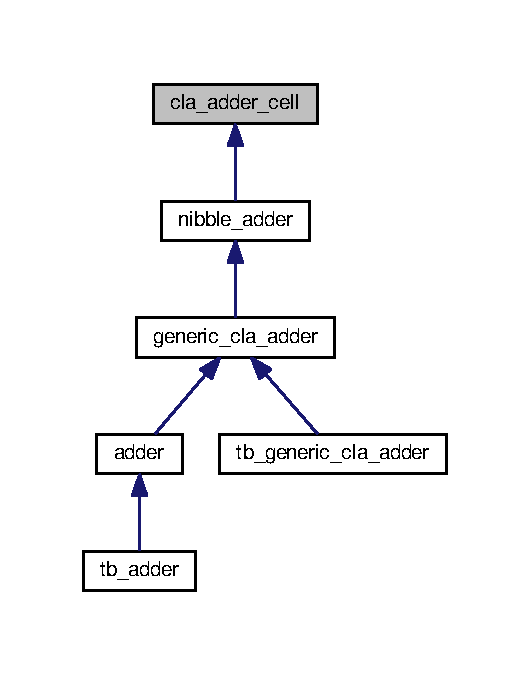
\includegraphics[width=326pt]{classcla__adder__cell__inherit__graph}
\end{center}
\end{figure}
\subsection*{Entities}
\begin{DoxyCompactItemize}
\item 
\hyperlink{classcla__adder__cell_1_1dataflow}{dataflow} architecture
\end{DoxyCompactItemize}
\subsection*{Ports}
 \begin{DoxyCompactItemize}
\item 
\hyperlink{group___base_cell_ga2b16ee1ce0d8ffb8f85ccea13f8ba38d}{add1}  {\bfseries {\bfseries \textcolor{vhdlchar}{in}\textcolor{vhdlchar}{ }}} {\bfseries \textcolor{vhdlchar}{std\+\_\+logic}\textcolor{vhdlchar}{ }} 
\begin{DoxyCompactList}\small\item\em addendo 1 \end{DoxyCompactList}\item 
\hyperlink{group___base_cell_gac3ebb689e34fc5e7657726b18d8b5369}{add2}  {\bfseries {\bfseries \textcolor{vhdlchar}{in}\textcolor{vhdlchar}{ }}} {\bfseries \textcolor{vhdlchar}{std\+\_\+logic}\textcolor{vhdlchar}{ }} 
\begin{DoxyCompactList}\small\item\em addendo 2 \end{DoxyCompactList}\item 
\hyperlink{group___base_cell_gaa556a73dc4a4de1a0d662b25adbcbe33}{carryin}  {\bfseries {\bfseries \textcolor{vhdlchar}{in}\textcolor{vhdlchar}{ }}} {\bfseries \textcolor{vhdlchar}{std\+\_\+logic}\textcolor{vhdlchar}{ }} 
\begin{DoxyCompactList}\small\item\em carry in ingresso \end{DoxyCompactList}\item 
\hyperlink{group___base_cell_gac94466f3a0e3e34f0231abcf4b667ade}{prop}  {\bfseries {\bfseries \textcolor{vhdlchar}{out}\textcolor{vhdlchar}{ }}} {\bfseries \textcolor{vhdlchar}{std\+\_\+logic}\textcolor{vhdlchar}{ }} 
\item 
\hyperlink{group___base_cell_gaad65a9c9ebd4dd83c2835249a1ba2dff}{gen}  {\bfseries {\bfseries \textcolor{vhdlchar}{out}\textcolor{vhdlchar}{ }}} {\bfseries \textcolor{vhdlchar}{std\+\_\+logic}\textcolor{vhdlchar}{ }} 
\item 
\hyperlink{group___base_cell_ga0d9fc1b21b42422b12d68ad73ca8ef13}{sum}  {\bfseries {\bfseries \textcolor{vhdlchar}{out}\textcolor{vhdlchar}{ }}} {\bfseries \textcolor{vhdlchar}{std\+\_\+logic}\textcolor{vhdlchar}{ }} 
\end{DoxyCompactItemize}


\subsection{Descrizione dettagliata}
Cella base di un addizionatore con carry-\/lookahead.

La cella somma tra loro due addendi ed un carry in ingresso, tutti espressi su un solo bit. Oltre a generare la somma, genera le funzioni \char`\"{}propagazione\char`\"{} e \char`\"{}generazione\char`\"{} del carry. 

La documentazione per questa classe è stata generata a partire dal seguente file\+:\begin{DoxyCompactItemize}
\item 
Src/adder/\hyperlink{cla__adder__cell_8vhd}{cla\+\_\+adder\+\_\+cell.\+vhd}\end{DoxyCompactItemize}

\hypertarget{classcla__carry__net}{\section{cla\+\_\+carry\+\_\+net Entity Reference}
\label{classcla__carry__net}\index{cla\+\_\+carry\+\_\+net@{cla\+\_\+carry\+\_\+net}}
}


Rete logica di calcolo dei riporti per un addizionatore a quattro bit con carry lookahead.

Permette di anticipare il calcolo dei riporti usando le funzioni \char`\"{}propagazione\char`\"{} e \char`\"{}generazione\char`\"{} prodotte dai singoli blocchi \hyperlink{classcla__adder__cell}{cla\+\_\+adder\+\_\+cell}, in modo da ridurre tempo necessario ad effettuare il calcolo di tutti i carry, quindi il tempo necessario a completare la somma. Questo blocco calcola solo i carry, pertanto va connesso ai blocchi \hyperlink{classcla__adder__cell}{cla\+\_\+adder\+\_\+cell}, per il calcolo materiale della somma, così come indicato dallo schema seguente, il quale rappresenta lo schema completo di un addizionatore a quattro bit\+: .  




Diagramma delle classi per cla\+\_\+carry\+\_\+net
\nopagebreak
\begin{figure}[H]
\begin{center}
\leavevmode
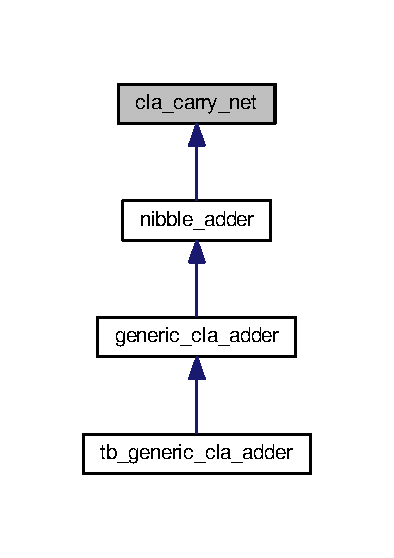
\includegraphics[width=255pt]{classcla__carry__net__inherit__graph}
\end{center}
\end{figure}
\subsection*{Entities}
\begin{DoxyCompactItemize}
\item 
\hyperlink{classcla__carry__net_1_1dataflow}{dataflow} architecture
\begin{DoxyCompactList}\small\item\em Implementazione dataflow dell'entita' \hyperlink{classcla__carry__net}{cla\+\_\+carry\+\_\+net}. \end{DoxyCompactList}\end{DoxyCompactItemize}
\subsection*{Ports}
 \begin{DoxyCompactItemize}
\item 
\hyperlink{group___carry_network_gac1f84cd3374a5a4d2ee2669ebdadafe8}{prop}  {\bfseries {\bfseries \textcolor{vhdlchar}{in}\textcolor{vhdlchar}{ }}} {\bfseries \textcolor{vhdlchar}{std\+\_\+logic\+\_\+vector}\textcolor{vhdlchar}{ }\textcolor{vhdlchar}{(}\textcolor{vhdlchar}{ }\textcolor{vhdlchar}{ } \textcolor{vhdldigit}{3} \textcolor{vhdlchar}{ }\textcolor{vhdlchar}{downto}\textcolor{vhdlchar}{ }\textcolor{vhdlchar}{ } \textcolor{vhdldigit}{0} \textcolor{vhdlchar}{ }\textcolor{vhdlchar}{)}\textcolor{vhdlchar}{ }} 
\begin{DoxyCompactList}\small\item\em funzione “propagazione” prodotta da \hyperlink{classcla__adder__cell}{cla\+\_\+adder\+\_\+cell}; vale 1 quando, sulla base degli ingressi, un adder propaghera' un eventuale carry in ingresso; prop(i) = add(i) O\+R add(i); in questo caso viene prodotta da quattro blocchi \hyperlink{classcla__adder__cell}{cla\+\_\+adder\+\_\+cell} sulla base dei loro ingressi \end{DoxyCompactList}\item 
\hyperlink{group___carry_network_ga1ff97daaf4e03defc21748593cacfaa7}{gen}  {\bfseries {\bfseries \textcolor{vhdlchar}{in}\textcolor{vhdlchar}{ }}} {\bfseries \textcolor{vhdlchar}{std\+\_\+logic\+\_\+vector}\textcolor{vhdlchar}{ }\textcolor{vhdlchar}{(}\textcolor{vhdlchar}{ }\textcolor{vhdlchar}{ } \textcolor{vhdldigit}{3} \textcolor{vhdlchar}{ }\textcolor{vhdlchar}{downto}\textcolor{vhdlchar}{ }\textcolor{vhdlchar}{ } \textcolor{vhdldigit}{0} \textcolor{vhdlchar}{ }\textcolor{vhdlchar}{)}\textcolor{vhdlchar}{ }} 
\begin{DoxyCompactList}\small\item\em funzione \char`\"{}generazione\char`\"{} prodotta da \hyperlink{classcla__adder__cell}{cla\+\_\+adder\+\_\+cell}; vale 1 quando, sulla base degli ingressi, un adder generera' un carry in uscita; gen(i) = add(i) A\+N\+D add(i); in questo caso viene prodotta da quattro blocchi \hyperlink{classcla__adder__cell}{cla\+\_\+adder\+\_\+cell} sulla base dei loro ingressi \end{DoxyCompactList}\item 
\hyperlink{group___carry_network_gaa556a73dc4a4de1a0d662b25adbcbe33}{carryin}  {\bfseries {\bfseries \textcolor{vhdlchar}{in}\textcolor{vhdlchar}{ }}} {\bfseries \textcolor{vhdlchar}{std\+\_\+logic}\textcolor{vhdlchar}{ }} 
\begin{DoxyCompactList}\small\item\em segnale di \char`\"{}carry-\/in\char`\"{}, prodotto da un eventuale \hyperlink{classcla__carry__net}{cla\+\_\+carry\+\_\+net} a monte. \end{DoxyCompactList}\item 
\hyperlink{group___carry_network_ga422e8e7ee01fc7ac7b7390cd2ad8c87b}{propin}  {\bfseries {\bfseries \textcolor{vhdlchar}{in}\textcolor{vhdlchar}{ }}} {\bfseries \textcolor{vhdlchar}{std\+\_\+logic}\textcolor{vhdlchar}{ }} 
\begin{DoxyCompactList}\small\item\em funzione \char`\"{}propagazione\char`\"{}, prodotta da una eventuale \hyperlink{classcla__carry__net}{cla\+\_\+carry\+\_\+net} a monte \end{DoxyCompactList}\item 
\hyperlink{group___carry_network_ga0a46d5193cb73eb993bc5d4f69741d0a}{genin}  {\bfseries {\bfseries \textcolor{vhdlchar}{in}\textcolor{vhdlchar}{ }}} {\bfseries \textcolor{vhdlchar}{std\+\_\+logic}\textcolor{vhdlchar}{ }} 
\begin{DoxyCompactList}\small\item\em funzione \char`\"{}generazione\char`\"{}, prodotta da una eventuale \hyperlink{classcla__carry__net}{cla\+\_\+carry\+\_\+net} a monte \end{DoxyCompactList}\item 
\hyperlink{group___carry_network_ga6b265f3fe41195485dfedd9824c3598f}{carryout}  {\bfseries {\bfseries \textcolor{vhdlchar}{out}\textcolor{vhdlchar}{ }}} {\bfseries \textcolor{vhdlchar}{std\+\_\+logic\+\_\+vector}\textcolor{vhdlchar}{ }\textcolor{vhdlchar}{(}\textcolor{vhdlchar}{ }\textcolor{vhdlchar}{ } \textcolor{vhdldigit}{3} \textcolor{vhdlchar}{ }\textcolor{vhdlchar}{downto}\textcolor{vhdlchar}{ }\textcolor{vhdlchar}{ } \textcolor{vhdldigit}{0} \textcolor{vhdlchar}{ }\textcolor{vhdlchar}{)}\textcolor{vhdlchar}{ }} 
\begin{DoxyCompactList}\small\item\em carry calcolati sulla base delle funzioni \char`\"{}propagazione\char`\"{} e \char`\"{}generazione\char`\"{} prodotti dai blocchi \hyperlink{classcla__adder__cell}{cla\+\_\+adder\+\_\+cell}, e sulla base delle funzioni \char`\"{}carry-\/in\char`\"{}, \char`\"{}propagazione\char`\"{} e \char`\"{}generazione\char`\"{} prodotti da eventuali blocchi a monte; ciascuno dei bit dovra' essere posto in ingresso ad un blocco \hyperlink{classcla__adder__cell}{cla\+\_\+adder\+\_\+cell} differente, affinche' possa essere calcolata la somma degli addendi \end{DoxyCompactList}\item 
\hyperlink{group___carry_network_ga5957c9cdd706cafd2da8855133a002c9}{propout}  {\bfseries {\bfseries \textcolor{vhdlchar}{out}\textcolor{vhdlchar}{ }}} {\bfseries \textcolor{vhdlchar}{std\+\_\+logic}\textcolor{vhdlchar}{ }} 
\begin{DoxyCompactList}\small\item\em funzione \char`\"{}propagazione\char`\"{} da porre in ingresso ad un eventuale blocco \hyperlink{classcla__carry__net}{cla\+\_\+carry\+\_\+net} a valle \end{DoxyCompactList}\item 
\hyperlink{group___carry_network_ga068cd5c4d23e284cb942702252ed1491}{genout}  {\bfseries {\bfseries \textcolor{vhdlchar}{out}\textcolor{vhdlchar}{ }}} {\bfseries \textcolor{vhdlchar}{std\+\_\+logic}\textcolor{vhdlchar}{ }} 
\begin{DoxyCompactList}\small\item\em funzione \char`\"{}generazione\char`\"{} da porre in ingresso ad un eventuale blocco \hyperlink{classcla__carry__net}{cla\+\_\+carry\+\_\+net} a valle \end{DoxyCompactList}\end{DoxyCompactItemize}


\subsection{Descrizione dettagliata}
Rete logica di calcolo dei riporti per un addizionatore a quattro bit con carry lookahead.

Permette di anticipare il calcolo dei riporti usando le funzioni \char`\"{}propagazione\char`\"{} e \char`\"{}generazione\char`\"{} prodotte dai singoli blocchi \hyperlink{classcla__adder__cell}{cla\+\_\+adder\+\_\+cell}, in modo da ridurre tempo necessario ad effettuare il calcolo di tutti i carry, quindi il tempo necessario a completare la somma. Questo blocco calcola solo i carry, pertanto va connesso ai blocchi \hyperlink{classcla__adder__cell}{cla\+\_\+adder\+\_\+cell}, per il calcolo materiale della somma, così come indicato dallo schema seguente, il quale rappresenta lo schema completo di un addizionatore a quattro bit\+: . 

La documentazione per questa classe è stata generata a partire dal seguente file\+:\begin{DoxyCompactItemize}
\item 
Src/adder/\hyperlink{cla__carry__net_8vhd}{cla\+\_\+carry\+\_\+net.\+vhd}\end{DoxyCompactItemize}

\hypertarget{classcla__adder__cell_1_1dataflow}{}\section{dataflow Architecture Reference}
\label{classcla__adder__cell_1_1dataflow}\index{dataflow@{dataflow}}


\subsection{Descrizione dettagliata}
funzione \char`\"{}somma\char`\"{}, rappresenta la somma tra gli addendi ed il carry in ingresso alla cella; sum = add1 X\+OR add2 X\+OR carryin; 

La documentazione per questa classe è stata generata a partire dal seguente file\+:\begin{DoxyCompactItemize}
\item 
Src/adder/\hyperlink{cla__adder__cell_8vhd}{cla\+\_\+adder\+\_\+cell.\+vhd}\end{DoxyCompactItemize}

\hypertarget{classtruncate_1_1dataflow}{\section{dataflow Architecture Reference}
\label{classtruncate_1_1dataflow}\index{dataflow@{dataflow}}
}


Implementazione dataflow dell'entity truncate.  


\subsection*{Constants}
 \begin{DoxyCompactItemize}
\item 
\hyperlink{classtruncate_1_1dataflow_a63701d8af27da7452a7588efcff357bc}{x} {\bfseries \textcolor{vhdlchar}{integer}\textcolor{vhdlchar}{ }\textcolor{vhdlchar}{ }\textcolor{vhdlchar}{\+:}\textcolor{vhdlchar}{=}\textcolor{vhdlchar}{ }\textcolor{vhdlchar}{ }\textcolor{vhdlchar}{ }\textcolor{vhdlchar}{ }{\bfseries \hyperlink{classtruncate_abe72b503b8140ab0d84911165e959b53}{s\+\_\+in\+\_\+int}} \textcolor{vhdlchar}{-\/}\textcolor{vhdlchar}{ }\textcolor{vhdlchar}{ }\textcolor{vhdlchar}{ }{\bfseries \hyperlink{classtruncate_a4ca792ca981e2f9d82bf36d9c82c08af}{s\+\_\+out\+\_\+int}} \textcolor{vhdlchar}{ }} 
\begin{DoxyCompactList}\small\item\em differenza, in termini di numero di bit usati per la rappresentazione della parte intera, tra formato di partenza e formato di arrivo \end{DoxyCompactList}\end{DoxyCompactItemize}
\subsection*{Signals}
 \begin{DoxyCompactItemize}
\item 
\hyperlink{classtruncate_1_1dataflow_ac257856843ad01f95857ccecfea5e47e}{padding\+\_\+pos} {\bfseries \textcolor{vhdlchar}{std\+\_\+logic\+\_\+vector}\textcolor{vhdlchar}{ }\textcolor{vhdlchar}{(}\textcolor{vhdlchar}{ }\textcolor{vhdlchar}{ }\textcolor{vhdlchar}{ }\textcolor{vhdlchar}{ }{\bfseries \hyperlink{classtruncate_1_1dataflow_a63701d8af27da7452a7588efcff357bc}{x}} \textcolor{vhdlchar}{-\/}\textcolor{vhdlchar}{ } \textcolor{vhdldigit}{1} \textcolor{vhdlchar}{ }\textcolor{vhdlchar}{downto}\textcolor{vhdlchar}{ }\textcolor{vhdlchar}{ } \textcolor{vhdldigit}{0} \textcolor{vhdlchar}{ }\textcolor{vhdlchar}{)}\textcolor{vhdlchar}{ }\textcolor{vhdlchar}{ }\textcolor{vhdlchar}{ }\textcolor{vhdlchar}{\+:}\textcolor{vhdlchar}{=}\textcolor{vhdlchar}{ }\textcolor{vhdlchar}{(}\textcolor{vhdlchar}{ }\textcolor{vhdlchar}{ }\textcolor{vhdlchar}{others}\textcolor{vhdlchar}{ }\textcolor{vhdlchar}{ }\textcolor{vhdlchar}{=}\textcolor{vhdlchar}{ }\textcolor{vhdlchar}{$>$}\textcolor{vhdlchar}{ }\textcolor{vhdlchar}{'}\textcolor{vhdlchar}{ } \textcolor{vhdldigit}{0} \textcolor{vhdlchar}{ }\textcolor{vhdlchar}{'}\textcolor{vhdlchar}{ }\textcolor{vhdlchar}{)}\textcolor{vhdlchar}{ }} 
\begin{DoxyCompactList}\small\item\em segnale di zero-\/padding, usato a seguito del troncamento, quando il numero di di bit usato per rappresentare la parte intera, nel formato di uscita, e' maggiore o uguale a zero. \end{DoxyCompactList}\item 
\hyperlink{classtruncate_1_1dataflow_a130836df2917c4b75d1fc24500082e76}{padding\+\_\+neg} {\bfseries \textcolor{vhdlchar}{std\+\_\+logic\+\_\+vector}\textcolor{vhdlchar}{ }\textcolor{vhdlchar}{(}\textcolor{vhdlchar}{ }\textcolor{vhdlchar}{ }\textcolor{vhdlchar}{ }\textcolor{vhdlchar}{ }{\bfseries \hyperlink{classtruncate_a8b62f8bfecb0fab845995b8b051101bc}{s\+\_\+out\+\_\+dim}} \textcolor{vhdlchar}{-\/}\textcolor{vhdlchar}{ } \textcolor{vhdldigit}{2} \textcolor{vhdlchar}{-\/}\textcolor{vhdlchar}{ }\textcolor{vhdlchar}{(}\textcolor{vhdlchar}{ }\textcolor{vhdlchar}{ }\textcolor{vhdlchar}{ }\textcolor{vhdlchar}{ }{\bfseries \hyperlink{classtruncate_ad3d18243ad6fe53a2277e2aa9b94ca45}{s\+\_\+in\+\_\+dim}} \textcolor{vhdlchar}{-\/}\textcolor{vhdlchar}{ }\textcolor{vhdlchar}{ }\textcolor{vhdlchar}{ }{\bfseries \hyperlink{classtruncate_1_1dataflow_a63701d8af27da7452a7588efcff357bc}{x}} \textcolor{vhdlchar}{ }\textcolor{vhdlchar}{)}\textcolor{vhdlchar}{ }\textcolor{vhdlchar}{ }\textcolor{vhdlchar}{downto}\textcolor{vhdlchar}{ }\textcolor{vhdlchar}{ } \textcolor{vhdldigit}{0} \textcolor{vhdlchar}{ }\textcolor{vhdlchar}{)}\textcolor{vhdlchar}{ }\textcolor{vhdlchar}{ }\textcolor{vhdlchar}{ }\textcolor{vhdlchar}{\+:}\textcolor{vhdlchar}{=}\textcolor{vhdlchar}{ }\textcolor{vhdlchar}{(}\textcolor{vhdlchar}{ }\textcolor{vhdlchar}{ }\textcolor{vhdlchar}{others}\textcolor{vhdlchar}{ }\textcolor{vhdlchar}{ }\textcolor{vhdlchar}{=}\textcolor{vhdlchar}{ }\textcolor{vhdlchar}{$>$}\textcolor{vhdlchar}{ }\textcolor{vhdlchar}{'}\textcolor{vhdlchar}{ } \textcolor{vhdldigit}{0} \textcolor{vhdlchar}{ }\textcolor{vhdlchar}{'}\textcolor{vhdlchar}{ }\textcolor{vhdlchar}{)}\textcolor{vhdlchar}{ }} 
\begin{DoxyCompactList}\small\item\em segnale di zero padding,, usato a seguito del troncamento, quando il numero di di bit usato per rappresentare la parte intera, nel formato di uscita, e' minore di zero. \end{DoxyCompactList}\end{DoxyCompactItemize}


\subsection{Detailed Description}
Implementazione dataflow dell'entity truncate. 

\paragraph*{Controllo dell'input}

Viene controllato che siano valide le seguenti assunzioni sui valori dei parametri generici\+:
\begin{DoxyItemize}
\item il numero totale di bit su cui e' espresso il segnale di ingresso non sia inferiore al numero di bit con cui viene espressa la parte frazionaria;
\item il numero totale di bit su cui verra' espresso il segnale di uscita non sia inferiore al numero di bit con cui verra' espressa la parte frazionaria;
\item il numero di bit totali su cui e' espresso il segnale di ingresso sia maggiore o uguale di quello sul quale verra' espresso il segnale di uscita;
\item il numero di bit su cui e' espressa la parte intera del segnale di ingresso non puo' essere minore di quella sul quale verra' espressa quella del segnale di uscita;
\end{DoxyItemize}

\paragraph*{Esecuzione del troncamento}

E' possibile distinguere due casi\+:
\begin{DoxyEnumerate}
\item il formato di destinazione ha numero di bit per esprimere la parte intera maggiore uguale di zero.~\newline
 In questo caso
\item il formato di destinazione ha numero di bit per esprimere la parte intera minore di zero.~\newline
 In questo caso
\end{DoxyEnumerate}

\begin{DoxyRefDesc}{Todo}
\item[\hyperlink{todo__todo000001}{Todo}]
\begin{DoxyItemize}
\item Definizione dei test-\/case
\item Scrittura del testbench
\item Esecuzione dei test
\item Trovare un modo per includere la documentazione interna ad architecture 
\end{DoxyItemize}\end{DoxyRefDesc}


\subsection{Member Data Documentation}
\hypertarget{classtruncate_1_1dataflow_a130836df2917c4b75d1fc24500082e76}{\index{truncate\+::dataflow@{truncate\+::dataflow}!padding\+\_\+neg@{padding\+\_\+neg}}
\index{padding\+\_\+neg@{padding\+\_\+neg}!truncate\+::dataflow@{truncate\+::dataflow}}
\subsubsection[{padding\+\_\+neg}]{\setlength{\rightskip}{0pt plus 5cm}{\bf padding\+\_\+neg} {\bfseries \textcolor{vhdlchar}{std\+\_\+logic\+\_\+vector}\textcolor{vhdlchar}{ }\textcolor{vhdlchar}{(}\textcolor{vhdlchar}{ }\textcolor{vhdlchar}{ }\textcolor{vhdlchar}{ }\textcolor{vhdlchar}{ }{\bfseries {\bf s\+\_\+out\+\_\+dim}} \textcolor{vhdlchar}{-\/}\textcolor{vhdlchar}{ } \textcolor{vhdldigit}{2} \textcolor{vhdlchar}{-\/}\textcolor{vhdlchar}{ }\textcolor{vhdlchar}{(}\textcolor{vhdlchar}{ }\textcolor{vhdlchar}{ }\textcolor{vhdlchar}{ }\textcolor{vhdlchar}{ }{\bfseries {\bf s\+\_\+in\+\_\+dim}} \textcolor{vhdlchar}{-\/}\textcolor{vhdlchar}{ }\textcolor{vhdlchar}{ }\textcolor{vhdlchar}{ }{\bfseries {\bf x}} \textcolor{vhdlchar}{ }\textcolor{vhdlchar}{)}\textcolor{vhdlchar}{ }\textcolor{vhdlchar}{ }\textcolor{vhdlchar}{downto}\textcolor{vhdlchar}{ }\textcolor{vhdlchar}{ } \textcolor{vhdldigit}{0} \textcolor{vhdlchar}{ }\textcolor{vhdlchar}{)}\textcolor{vhdlchar}{ }\textcolor{vhdlchar}{ }\textcolor{vhdlchar}{ }\textcolor{vhdlchar}{\+:}\textcolor{vhdlchar}{=}\textcolor{vhdlchar}{ }\textcolor{vhdlchar}{(}\textcolor{vhdlchar}{ }\textcolor{vhdlchar}{ }\textcolor{vhdlchar}{others}\textcolor{vhdlchar}{ }\textcolor{vhdlchar}{ }\textcolor{vhdlchar}{=}\textcolor{vhdlchar}{ }\textcolor{vhdlchar}{$>$}\textcolor{vhdlchar}{ }\textcolor{vhdlchar}{'}\textcolor{vhdlchar}{ } \textcolor{vhdldigit}{0} \textcolor{vhdlchar}{ }\textcolor{vhdlchar}{'}\textcolor{vhdlchar}{ }\textcolor{vhdlchar}{)}\textcolor{vhdlchar}{ }} \hspace{0.3cm}{\ttfamily [Signal]}}}\label{classtruncate_1_1dataflow_a130836df2917c4b75d1fc24500082e76}


segnale di zero padding,, usato a seguito del troncamento, quando il numero di di bit usato per rappresentare la parte intera, nel formato di uscita, e' minore di zero. 

\hypertarget{classtruncate_1_1dataflow_ac257856843ad01f95857ccecfea5e47e}{\index{truncate\+::dataflow@{truncate\+::dataflow}!padding\+\_\+pos@{padding\+\_\+pos}}
\index{padding\+\_\+pos@{padding\+\_\+pos}!truncate\+::dataflow@{truncate\+::dataflow}}
\subsubsection[{padding\+\_\+pos}]{\setlength{\rightskip}{0pt plus 5cm}{\bf padding\+\_\+pos} {\bfseries \textcolor{vhdlchar}{std\+\_\+logic\+\_\+vector}\textcolor{vhdlchar}{ }\textcolor{vhdlchar}{(}\textcolor{vhdlchar}{ }\textcolor{vhdlchar}{ }\textcolor{vhdlchar}{ }\textcolor{vhdlchar}{ }{\bfseries {\bf x}} \textcolor{vhdlchar}{-\/}\textcolor{vhdlchar}{ } \textcolor{vhdldigit}{1} \textcolor{vhdlchar}{ }\textcolor{vhdlchar}{downto}\textcolor{vhdlchar}{ }\textcolor{vhdlchar}{ } \textcolor{vhdldigit}{0} \textcolor{vhdlchar}{ }\textcolor{vhdlchar}{)}\textcolor{vhdlchar}{ }\textcolor{vhdlchar}{ }\textcolor{vhdlchar}{ }\textcolor{vhdlchar}{\+:}\textcolor{vhdlchar}{=}\textcolor{vhdlchar}{ }\textcolor{vhdlchar}{(}\textcolor{vhdlchar}{ }\textcolor{vhdlchar}{ }\textcolor{vhdlchar}{others}\textcolor{vhdlchar}{ }\textcolor{vhdlchar}{ }\textcolor{vhdlchar}{=}\textcolor{vhdlchar}{ }\textcolor{vhdlchar}{$>$}\textcolor{vhdlchar}{ }\textcolor{vhdlchar}{'}\textcolor{vhdlchar}{ } \textcolor{vhdldigit}{0} \textcolor{vhdlchar}{ }\textcolor{vhdlchar}{'}\textcolor{vhdlchar}{ }\textcolor{vhdlchar}{)}\textcolor{vhdlchar}{ }} \hspace{0.3cm}{\ttfamily [Signal]}}}\label{classtruncate_1_1dataflow_ac257856843ad01f95857ccecfea5e47e}


segnale di zero-\/padding, usato a seguito del troncamento, quando il numero di di bit usato per rappresentare la parte intera, nel formato di uscita, e' maggiore o uguale a zero. 

\hypertarget{classtruncate_1_1dataflow_a63701d8af27da7452a7588efcff357bc}{\index{truncate\+::dataflow@{truncate\+::dataflow}!x@{x}}
\index{x@{x}!truncate\+::dataflow@{truncate\+::dataflow}}
\subsubsection[{x}]{\setlength{\rightskip}{0pt plus 5cm}{\bf x} {\bfseries \textcolor{vhdlchar}{integer}\textcolor{vhdlchar}{ }\textcolor{vhdlchar}{ }\textcolor{vhdlchar}{\+:}\textcolor{vhdlchar}{=}\textcolor{vhdlchar}{ }\textcolor{vhdlchar}{ }\textcolor{vhdlchar}{ }\textcolor{vhdlchar}{ }{\bfseries {\bf s\+\_\+in\+\_\+int}} \textcolor{vhdlchar}{-\/}\textcolor{vhdlchar}{ }\textcolor{vhdlchar}{ }\textcolor{vhdlchar}{ }{\bfseries {\bf s\+\_\+out\+\_\+int}} \textcolor{vhdlchar}{ }} \hspace{0.3cm}{\ttfamily [Constant]}}}\label{classtruncate_1_1dataflow_a63701d8af27da7452a7588efcff357bc}


differenza, in termini di numero di bit usati per la rappresentazione della parte intera, tra formato di partenza e formato di arrivo 



The documentation for this class was generated from the following file\+:\begin{DoxyCompactItemize}
\item 
Src/\hyperlink{truncate_8vhd}{truncate.\+vhd}\end{DoxyCompactItemize}

\hypertarget{classcla__carry__net_1_1dataflow}{\section{dataflow Architecture Reference}
\label{classcla__carry__net_1_1dataflow}\index{dataflow@{dataflow}}
}


Implementazione dataflow dell'entita' \hyperlink{classcla__carry__net}{cla\+\_\+carry\+\_\+net}.  




\subsection{Descrizione dettagliata}
Implementazione dataflow dell'entita' \hyperlink{classcla__carry__net}{cla\+\_\+carry\+\_\+net}. 

L'implementazione si basa sul seguente ragionamento\+: Proviamo ad esprimere, adesso, il carry carryout(i+1) in base alle funzioni gen(i) e prop(i), partendo, ad esempio, da carryout(1). Il carry carryout(0) varra' 1 se al passo precedente è stato generato riporto oppure se verra' propagato il carry carryin. In formule\+: \begin{center}carryout(0)=genin+(propin$\ast$carryin);\end{center}  Possiamo estendere lo stesso ragionamento a carryout(2)\+: \begin{center}carryout(1)=gen(1)+prop(1)$\ast$carryout(1)=gen(1)+prop(1)$\ast$gen(0)+prop(1)$\ast$prop(0)$\ast$carryin\end{center}  Cio' significa che il riporto carryout(1) lo si può esprimere sulla base di soli dati di ingresso con reti combinatorie a due livelli, senza utilizzare valori calcolati da nodi precedenti. Tutto ciò si traduce in un minor tempo necessario ad effettuare il calcolo di tutti i carry, quindi un minor tempo necessario a completare la somma. Purtroppo non si può procedere in questo modo ad oltranza per cui si tende a spezzare" la rete per il calcolo dei carry in blocchi più piccoli, ad esempio reti per il calcolo di carry per quattro bit. Considerando che \begin{center}carryout(4)=gen(3)+prop(3)$\ast$carryout(3)=...=genout+propout$\ast$carryin\end{center}  con \begin{center}genout=gen(3)+(prop(3)$\ast$gen(2))+(prop(3)$\ast$prop(2)$\ast$gen(1))+(prop(3)$\ast$prop(2)$\ast$prop(1)$\ast$gen(0))+(prop(3)$\ast$prop(2)$\ast$prop(1)$\ast$prop(0)$\ast$genin)\end{center}  \begin{center}propout=prop(3)$\ast$prop(2)$\ast$prop(1)$\ast$prop(0)$\ast$propin\end{center}  Si può costruire dei blocchi che presentino in uscita i segnali genout e propout, in modo da permettere ad eventuali blocchi successivi il calcolo veloce dei carry sulla base di questi segnali e del segnale carryin. 

La documentazione per questa classe è stata generata a partire dal seguente file\+:\begin{DoxyCompactItemize}
\item 
Src/adder/\hyperlink{cla__carry__net_8vhd}{cla\+\_\+carry\+\_\+net.\+vhd}\end{DoxyCompactItemize}

\hypertarget{classgeneric__cla__adder}{}\section{generic\+\_\+cla\+\_\+adder Entity Reference}
\label{classgeneric__cla__adder}\index{generic\+\_\+cla\+\_\+adder@{generic\+\_\+cla\+\_\+adder}}


Adder custom con carry-\/lookahead

\hyperlink{classgeneric__cla__adder}{generic\+\_\+cla\+\_\+adder} somma tra loro due addendi ed un carry in ingresso; gli addendi sono espressi su multipli interi di quattro bit. Oltre a generare la somma, genera il flag di carry ed il flag di overflow.  




Diagramma delle classi per generic\+\_\+cla\+\_\+adder
\nopagebreak
\begin{figure}[H]
\begin{center}
\leavevmode
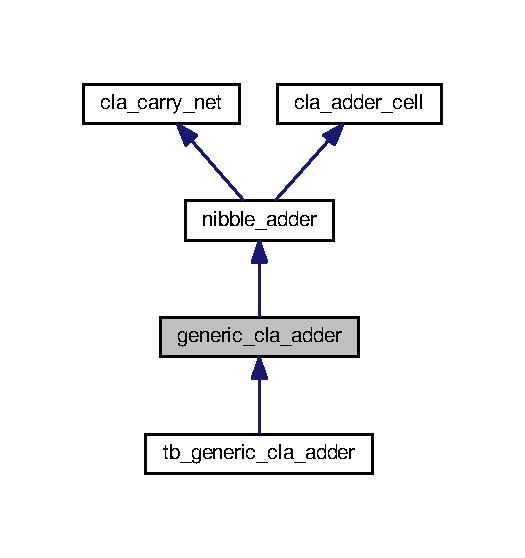
\includegraphics[width=319pt]{classgeneric__cla__adder__inherit__graph}
\end{center}
\end{figure}


Diagramma di collaborazione per generic\+\_\+cla\+\_\+adder\+:\nopagebreak
\begin{figure}[H]
\begin{center}
\leavevmode
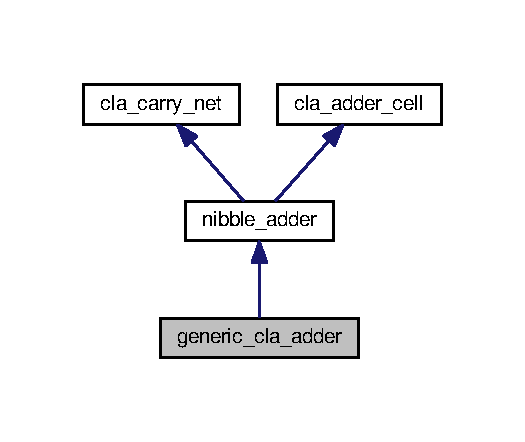
\includegraphics[width=252pt]{classgeneric__cla__adder__coll__graph}
\end{center}
\end{figure}
\subsection*{Entities}
\begin{DoxyCompactItemize}
\item 
\hyperlink{classgeneric__cla__adder_1_1structural}{structural} architecture
\begin{DoxyCompactList}\small\item\em Implementazione structural di \hyperlink{classgeneric__cla__adder}{generic\+\_\+cla\+\_\+adder}.

Questa implementazione istanzia tanti blocchi \hyperlink{classnibble__adder}{nibble\+\_\+adder} quanti siano i nibble in cui sono rappresentati gli addendi. La somma è espressa sullo stesso numero di bit. I diversi blocchi sono connessi tra loro come indicato nello schema ricordato di seguito\+: . \end{DoxyCompactList}\end{DoxyCompactItemize}
\subsection*{Generics}
 \begin{DoxyCompactItemize}
\item 
\hyperlink{group___carry_loockahead_ga0b63b586531492d0fa882246cca071c1}{nibbles} {\bfseries {\bfseries \textcolor{vhdlchar}{natural}\textcolor{vhdlchar}{ }\textcolor{vhdlchar}{ }\textcolor{vhdlchar}{\+:}\textcolor{vhdlchar}{=}\textcolor{vhdlchar}{ }\textcolor{vhdlchar}{ } \textcolor{vhdldigit}{2} \textcolor{vhdlchar}{ }}}
\end{DoxyCompactItemize}
\subsection*{Ports}
 \begin{DoxyCompactItemize}
\item 
\hyperlink{group___carry_loockahead_ga1c211cdf2d4cf97e869c442832c53439}{carry\+\_\+in}  {\bfseries {\bfseries \textcolor{vhdlchar}{in}\textcolor{vhdlchar}{ }}} {\bfseries \textcolor{vhdlchar}{std\+\_\+logic}\textcolor{vhdlchar}{ }} 
\item 
\hyperlink{group___carry_loockahead_gae4a2e124144a2f35270a55f0cf32a5ee}{addendum1}  {\bfseries {\bfseries \textcolor{vhdlchar}{in}\textcolor{vhdlchar}{ }}} {\bfseries \textcolor{vhdlchar}{std\+\_\+logic\+\_\+vector}\textcolor{vhdlchar}{ }\textcolor{vhdlchar}{(}\textcolor{vhdlchar}{ }\textcolor{vhdlchar}{(}\textcolor{vhdlchar}{ }\textcolor{vhdlchar}{ }\textcolor{vhdlchar}{ }\textcolor{vhdlchar}{ }{\bfseries \hyperlink{group___carry_loockahead_ga0b63b586531492d0fa882246cca071c1}{nibbles}} \textcolor{vhdlchar}{$\ast$}\textcolor{vhdlchar}{ } \textcolor{vhdldigit}{4} \textcolor{vhdlchar}{ }\textcolor{vhdlchar}{)}\textcolor{vhdlchar}{ }\textcolor{vhdlchar}{-\/}\textcolor{vhdlchar}{ } \textcolor{vhdldigit}{1} \textcolor{vhdlchar}{ }\textcolor{vhdlchar}{downto}\textcolor{vhdlchar}{ }\textcolor{vhdlchar}{ } \textcolor{vhdldigit}{0} \textcolor{vhdlchar}{ }\textcolor{vhdlchar}{)}\textcolor{vhdlchar}{ }} 
\begin{DoxyCompactList}\small\item\em addendo 1, espresso in complemento a due \end{DoxyCompactList}\item 
\hyperlink{group___carry_loockahead_ga2715463c615cf8418f85c6a1427ce62c}{addendum2}  {\bfseries {\bfseries \textcolor{vhdlchar}{in}\textcolor{vhdlchar}{ }}} {\bfseries \textcolor{vhdlchar}{std\+\_\+logic\+\_\+vector}\textcolor{vhdlchar}{ }\textcolor{vhdlchar}{(}\textcolor{vhdlchar}{ }\textcolor{vhdlchar}{(}\textcolor{vhdlchar}{ }\textcolor{vhdlchar}{ }\textcolor{vhdlchar}{ }\textcolor{vhdlchar}{ }{\bfseries \hyperlink{group___carry_loockahead_ga0b63b586531492d0fa882246cca071c1}{nibbles}} \textcolor{vhdlchar}{$\ast$}\textcolor{vhdlchar}{ } \textcolor{vhdldigit}{4} \textcolor{vhdlchar}{ }\textcolor{vhdlchar}{)}\textcolor{vhdlchar}{ }\textcolor{vhdlchar}{-\/}\textcolor{vhdlchar}{ } \textcolor{vhdldigit}{1} \textcolor{vhdlchar}{ }\textcolor{vhdlchar}{downto}\textcolor{vhdlchar}{ }\textcolor{vhdlchar}{ } \textcolor{vhdldigit}{0} \textcolor{vhdlchar}{ }\textcolor{vhdlchar}{)}\textcolor{vhdlchar}{ }} 
\begin{DoxyCompactList}\small\item\em addendo 2, espresso in complemento a due \end{DoxyCompactList}\item 
\hyperlink{group___carry_loockahead_ga1b4798a9e96bb32e9c08ce68e24e7871}{sum}  {\bfseries {\bfseries \textcolor{vhdlchar}{out}\textcolor{vhdlchar}{ }}} {\bfseries \textcolor{vhdlchar}{std\+\_\+logic\+\_\+vector}\textcolor{vhdlchar}{ }\textcolor{vhdlchar}{(}\textcolor{vhdlchar}{ }\textcolor{vhdlchar}{(}\textcolor{vhdlchar}{ }\textcolor{vhdlchar}{ }\textcolor{vhdlchar}{ }\textcolor{vhdlchar}{ }{\bfseries \hyperlink{group___carry_loockahead_ga0b63b586531492d0fa882246cca071c1}{nibbles}} \textcolor{vhdlchar}{$\ast$}\textcolor{vhdlchar}{ } \textcolor{vhdldigit}{4} \textcolor{vhdlchar}{ }\textcolor{vhdlchar}{)}\textcolor{vhdlchar}{ }\textcolor{vhdlchar}{-\/}\textcolor{vhdlchar}{ } \textcolor{vhdldigit}{1} \textcolor{vhdlchar}{ }\textcolor{vhdlchar}{downto}\textcolor{vhdlchar}{ }\textcolor{vhdlchar}{ } \textcolor{vhdldigit}{0} \textcolor{vhdlchar}{ }\textcolor{vhdlchar}{)}\textcolor{vhdlchar}{ }} 
\begin{DoxyCompactList}\small\item\em somma degli addendi, espressa in complemento a due \end{DoxyCompactList}\item 
\hyperlink{group___carry_loockahead_ga851aaea297bdc862fba5478c4bf0e214}{carry\+\_\+out}  {\bfseries {\bfseries \textcolor{vhdlchar}{out}\textcolor{vhdlchar}{ }}} {\bfseries \textcolor{vhdlchar}{std\+\_\+logic}\textcolor{vhdlchar}{ }} 
\item 
\hyperlink{group___carry_loockahead_ga9650307dde287e0bcfa1e26370c006c2}{overflow}  {\bfseries {\bfseries \textcolor{vhdlchar}{out}\textcolor{vhdlchar}{ }}} {\bfseries \textcolor{vhdlchar}{std\+\_\+logic}\textcolor{vhdlchar}{ }} 
\end{DoxyCompactItemize}


\subsection{Descrizione dettagliata}
Adder custom con carry-\/lookahead

\hyperlink{classgeneric__cla__adder}{generic\+\_\+cla\+\_\+adder} somma tra loro due addendi ed un carry in ingresso; gli addendi sono espressi su multipli interi di quattro bit. Oltre a generare la somma, genera il flag di carry ed il flag di overflow. 

La documentazione per questa classe è stata generata a partire dal seguente file\+:\begin{DoxyCompactItemize}
\item 
Src/adder/\hyperlink{generic__cla__adder_8vhd}{generic\+\_\+cla\+\_\+adder.\+vhd}\end{DoxyCompactItemize}

\hypertarget{classnibble__adder}{}\section{nibble\+\_\+adder Entity Reference}
\label{classnibble__adder}\index{nibble\+\_\+adder@{nibble\+\_\+adder}}


Addizionatore con carry-\/lookahead a quattro bit.

La cella somma tra loro due addendi ed un carry in ingresso; gli addendi sono espressi su quattro bit. Oltre a generare la somma, genera le funzioni \char`\"{}propagazione\char`\"{} e \char`\"{}generazione\char`\"{} del carry per eventuali blocchi \hyperlink{classnibble__adder}{nibble\+\_\+adder} posti a valle.  




Diagramma delle classi per nibble\+\_\+adder
\nopagebreak
\begin{figure}[H]
\begin{center}
\leavevmode
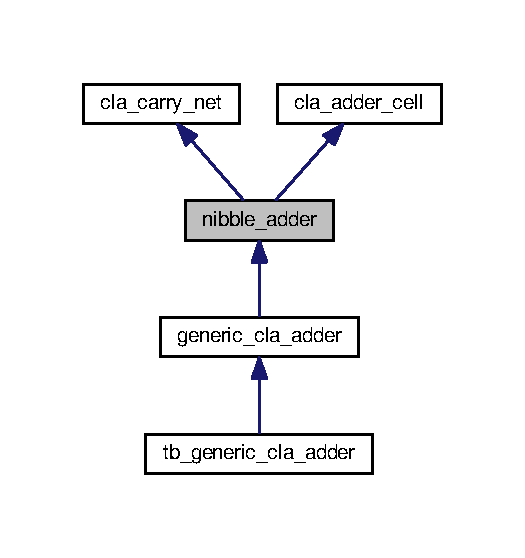
\includegraphics[width=319pt]{classnibble__adder__inherit__graph}
\end{center}
\end{figure}


Diagramma di collaborazione per nibble\+\_\+adder\+:
\nopagebreak
\begin{figure}[H]
\begin{center}
\leavevmode
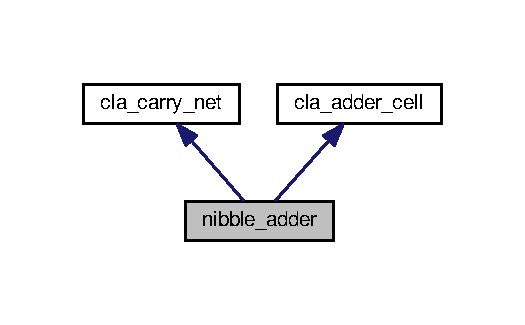
\includegraphics[width=252pt]{classnibble__adder__coll__graph}
\end{center}
\end{figure}
\subsection*{Entities}
\begin{DoxyCompactItemize}
\item 
\hyperlink{classnibble__adder_1_1structural}{structural} architecture
\begin{DoxyCompactList}\small\item\em Implementazione structural dell\textquotesingle{}entità \hyperlink{classnibble__adder}{nibble\+\_\+adder}.

Questa architettura istanzia una entità \hyperlink{classcla__carry__net}{cla\+\_\+carry\+\_\+net} ed una entità \hyperlink{classcla__adder__cell}{cla\+\_\+adder\+\_\+cell} per ogni bit su cui sono espressi gli addendi, connettendoli tra loro secondo lo schema riportato di seguito\+: . \end{DoxyCompactList}\end{DoxyCompactItemize}
\subsection*{Ports}
 \begin{DoxyCompactItemize}
\item 
\hyperlink{group___nibble_adder_ga2c8945f4747b9a5448412c95fc281c87}{addendum1}  {\bfseries {\bfseries \textcolor{vhdlchar}{in}\textcolor{vhdlchar}{ }}} {\bfseries \textcolor{vhdlchar}{std\+\_\+logic\+\_\+vector}\textcolor{vhdlchar}{ }\textcolor{vhdlchar}{(}\textcolor{vhdlchar}{ }\textcolor{vhdlchar}{ } \textcolor{vhdldigit}{3} \textcolor{vhdlchar}{ }\textcolor{vhdlchar}{downto}\textcolor{vhdlchar}{ }\textcolor{vhdlchar}{ } \textcolor{vhdldigit}{0} \textcolor{vhdlchar}{ }\textcolor{vhdlchar}{)}\textcolor{vhdlchar}{ }} 
\begin{DoxyCompactList}\small\item\em addendo 1 \end{DoxyCompactList}\item 
\hyperlink{group___nibble_adder_gad1fa6d9d78208885ad2f4c417fc4b530}{addendum2}  {\bfseries {\bfseries \textcolor{vhdlchar}{in}\textcolor{vhdlchar}{ }}} {\bfseries \textcolor{vhdlchar}{std\+\_\+logic\+\_\+vector}\textcolor{vhdlchar}{ }\textcolor{vhdlchar}{(}\textcolor{vhdlchar}{ }\textcolor{vhdlchar}{ } \textcolor{vhdldigit}{3} \textcolor{vhdlchar}{ }\textcolor{vhdlchar}{downto}\textcolor{vhdlchar}{ }\textcolor{vhdlchar}{ } \textcolor{vhdldigit}{0} \textcolor{vhdlchar}{ }\textcolor{vhdlchar}{)}\textcolor{vhdlchar}{ }} 
\begin{DoxyCompactList}\small\item\em addendo 2 \end{DoxyCompactList}\item 
\hyperlink{group___nibble_adder_gaa556a73dc4a4de1a0d662b25adbcbe33}{carryin}  {\bfseries {\bfseries \textcolor{vhdlchar}{in}\textcolor{vhdlchar}{ }}} {\bfseries \textcolor{vhdlchar}{std\+\_\+logic}\textcolor{vhdlchar}{ }} 
\begin{DoxyCompactList}\small\item\em segnale di \char`\"{}carry-\/in\char`\"{}, prodotto da un eventuale \hyperlink{classnibble__adder}{nibble\+\_\+adder} a monte. \end{DoxyCompactList}\item 
\hyperlink{group___nibble_adder_ga422e8e7ee01fc7ac7b7390cd2ad8c87b}{propin}  {\bfseries {\bfseries \textcolor{vhdlchar}{in}\textcolor{vhdlchar}{ }}} {\bfseries \textcolor{vhdlchar}{std\+\_\+logic}\textcolor{vhdlchar}{ }} 
\begin{DoxyCompactList}\small\item\em funzione \char`\"{}propagazione\char`\"{}, prodotta da una eventuale \hyperlink{classnibble__adder}{nibble\+\_\+adder} a monte \end{DoxyCompactList}\item 
\hyperlink{group___nibble_adder_ga0a46d5193cb73eb993bc5d4f69741d0a}{genin}  {\bfseries {\bfseries \textcolor{vhdlchar}{in}\textcolor{vhdlchar}{ }}} {\bfseries \textcolor{vhdlchar}{std\+\_\+logic}\textcolor{vhdlchar}{ }} 
\begin{DoxyCompactList}\small\item\em funzione \char`\"{}generazione\char`\"{}, prodotta da una eventuale \hyperlink{classnibble__adder}{nibble\+\_\+adder} a monte \end{DoxyCompactList}\item 
\hyperlink{group___nibble_adder_ga5957c9cdd706cafd2da8855133a002c9}{propout}  {\bfseries {\bfseries \textcolor{vhdlchar}{out}\textcolor{vhdlchar}{ }}} {\bfseries \textcolor{vhdlchar}{std\+\_\+logic}\textcolor{vhdlchar}{ }} 
\item 
\hyperlink{group___nibble_adder_ga068cd5c4d23e284cb942702252ed1491}{genout}  {\bfseries {\bfseries \textcolor{vhdlchar}{out}\textcolor{vhdlchar}{ }}} {\bfseries \textcolor{vhdlchar}{std\+\_\+logic}\textcolor{vhdlchar}{ }} 
\item 
\hyperlink{group___nibble_adder_gadfe538323c3296159dd3b383325a996b}{sum}  {\bfseries {\bfseries \textcolor{vhdlchar}{out}\textcolor{vhdlchar}{ }}} {\bfseries \textcolor{vhdlchar}{std\+\_\+logic\+\_\+vector}\textcolor{vhdlchar}{ }\textcolor{vhdlchar}{(}\textcolor{vhdlchar}{ }\textcolor{vhdlchar}{ } \textcolor{vhdldigit}{3} \textcolor{vhdlchar}{ }\textcolor{vhdlchar}{downto}\textcolor{vhdlchar}{ }\textcolor{vhdlchar}{ } \textcolor{vhdldigit}{0} \textcolor{vhdlchar}{ }\textcolor{vhdlchar}{)}\textcolor{vhdlchar}{ }} 
\end{DoxyCompactItemize}


\subsection{Descrizione dettagliata}
Addizionatore con carry-\/lookahead a quattro bit.

La cella somma tra loro due addendi ed un carry in ingresso; gli addendi sono espressi su quattro bit. Oltre a generare la somma, genera le funzioni \char`\"{}propagazione\char`\"{} e \char`\"{}generazione\char`\"{} del carry per eventuali blocchi \hyperlink{classnibble__adder}{nibble\+\_\+adder} posti a valle. 

La documentazione per questa classe è stata generata a partire dal seguente file\+:\begin{DoxyCompactItemize}
\item 
Src/adder/\hyperlink{nibble__adder_8vhd}{nibble\+\_\+adder.\+vhd}\end{DoxyCompactItemize}

\hypertarget{classprova}{\section{prova Entity Reference}
\label{classprova}\index{prova@{prova}}
}


Diagramma delle classi per prova\nopagebreak
\begin{figure}[H]
\begin{center}
\leavevmode
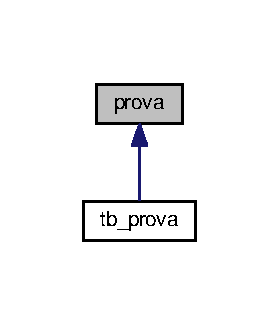
\includegraphics[width=134pt]{classprova__inherit__graph}
\end{center}
\end{figure}
\subsection*{Entities}
\begin{DoxyCompactItemize}
\item 
\hyperlink{classprova_1_1_behavioral}{Behavioral} architecture
\end{DoxyCompactItemize}
\subsection*{Libraries}
 \begin{DoxyCompactItemize}
\item 
\hyperlink{classprova_ae4f03c286607f3181e16b9aa12d0c6d4}{I\+E\+E\+E} 
\end{DoxyCompactItemize}
\subsection*{Use Clauses}
 \begin{DoxyCompactItemize}
\item 
\hyperlink{classprova_aa4b2b25246a821511120e3149b003563}{S\+T\+D\+\_\+\+L\+O\+G\+I\+C\+\_\+1164}   
\item 
\hyperlink{classprova_ae00f3f04545af57582ff10609eee23e2}{N\+U\+M\+E\+R\+I\+C\+\_\+\+S\+T\+D}   
\end{DoxyCompactItemize}
\subsection*{Generics}
 \begin{DoxyCompactItemize}
\item 
\hyperlink{classprova_a8dc284505c594faf4f1ce84af80f854b}{m} {\bfseries {\bfseries \textcolor{vhdlchar}{natural}\textcolor{vhdlchar}{ }\textcolor{vhdlchar}{ }\textcolor{vhdlchar}{\+:}\textcolor{vhdlchar}{=}\textcolor{vhdlchar}{ }\textcolor{vhdlchar}{ } \textcolor{vhdldigit}{24} \textcolor{vhdlchar}{ }}}
\item 
\hyperlink{classprova_ade9247ceba0e4ec66dc5c18b00acc9ff}{n} {\bfseries {\bfseries \textcolor{vhdlchar}{natural}\textcolor{vhdlchar}{ }\textcolor{vhdlchar}{ }\textcolor{vhdlchar}{\+:}\textcolor{vhdlchar}{=}\textcolor{vhdlchar}{ }\textcolor{vhdlchar}{ } \textcolor{vhdldigit}{20} \textcolor{vhdlchar}{ }}}
\end{DoxyCompactItemize}
\subsection*{Ports}
 \begin{DoxyCompactItemize}
\item 
\hyperlink{classprova_adb70646863893ceb3fdfd4174ed8ff46}{x}  {\bfseries {\bfseries \textcolor{vhdlchar}{in}\textcolor{vhdlchar}{ }}} {\bfseries \textcolor{vhdlchar}{S\+T\+D\+\_\+\+L\+O\+G\+I\+C\+\_\+\+V\+E\+C\+T\+O\+R}\textcolor{vhdlchar}{ }\textcolor{vhdlchar}{(}\textcolor{vhdlchar}{ }\textcolor{vhdlchar}{ }\textcolor{vhdlchar}{ }\textcolor{vhdlchar}{ }{\bfseries \hyperlink{classprova_a8dc284505c594faf4f1ce84af80f854b}{m}} \textcolor{vhdlchar}{-\/}\textcolor{vhdlchar}{ } \textcolor{vhdldigit}{1} \textcolor{vhdlchar}{ }\textcolor{vhdlchar}{downto}\textcolor{vhdlchar}{ }\textcolor{vhdlchar}{ } \textcolor{vhdldigit}{0} \textcolor{vhdlchar}{ }\textcolor{vhdlchar}{)}\textcolor{vhdlchar}{ }} 
\item 
\hyperlink{classprova_a7b9da25245767111877eb06273992a1a}{y}  {\bfseries {\bfseries \textcolor{vhdlchar}{in}\textcolor{vhdlchar}{ }}} {\bfseries \textcolor{vhdlchar}{S\+T\+D\+\_\+\+L\+O\+G\+I\+C\+\_\+\+V\+E\+C\+T\+O\+R}\textcolor{vhdlchar}{ }\textcolor{vhdlchar}{(}\textcolor{vhdlchar}{ }\textcolor{vhdlchar}{ }\textcolor{vhdlchar}{ }\textcolor{vhdlchar}{ }{\bfseries \hyperlink{classprova_ade9247ceba0e4ec66dc5c18b00acc9ff}{n}} \textcolor{vhdlchar}{-\/}\textcolor{vhdlchar}{ } \textcolor{vhdldigit}{1} \textcolor{vhdlchar}{ }\textcolor{vhdlchar}{downto}\textcolor{vhdlchar}{ }\textcolor{vhdlchar}{ } \textcolor{vhdldigit}{0} \textcolor{vhdlchar}{ }\textcolor{vhdlchar}{)}\textcolor{vhdlchar}{ }} 
\item 
\hyperlink{classprova_a3e8d3b9c7a9b55176b2b30f94d1f5744}{prod}  {\bfseries {\bfseries \textcolor{vhdlchar}{out}\textcolor{vhdlchar}{ }}} {\bfseries \textcolor{vhdlchar}{S\+T\+D\+\_\+\+L\+O\+G\+I\+C\+\_\+\+V\+E\+C\+T\+O\+R}\textcolor{vhdlchar}{ }\textcolor{vhdlchar}{(}\textcolor{vhdlchar}{ }\textcolor{vhdlchar}{ }\textcolor{vhdlchar}{ }\textcolor{vhdlchar}{ }{\bfseries \hyperlink{classprova_a8dc284505c594faf4f1ce84af80f854b}{m}} \textcolor{vhdlchar}{+}\textcolor{vhdlchar}{ }\textcolor{vhdlchar}{ }\textcolor{vhdlchar}{ }{\bfseries \hyperlink{classprova_ade9247ceba0e4ec66dc5c18b00acc9ff}{n}} \textcolor{vhdlchar}{-\/}\textcolor{vhdlchar}{ } \textcolor{vhdldigit}{1} \textcolor{vhdlchar}{ }\textcolor{vhdlchar}{downto}\textcolor{vhdlchar}{ }\textcolor{vhdlchar}{ } \textcolor{vhdldigit}{0} \textcolor{vhdlchar}{ }\textcolor{vhdlchar}{)}\textcolor{vhdlchar}{ }} 
\end{DoxyCompactItemize}


\subsection{Documentazione dei membri dato}
\hypertarget{classprova_ae4f03c286607f3181e16b9aa12d0c6d4}{\index{prova@{prova}!I\+E\+E\+E@{I\+E\+E\+E}}
\index{I\+E\+E\+E@{I\+E\+E\+E}!prova@{prova}}
\subsubsection[{I\+E\+E\+E}]{\setlength{\rightskip}{0pt plus 5cm}{\bf I\+E\+E\+E}\hspace{0.3cm}{\ttfamily [Library]}}}\label{classprova_ae4f03c286607f3181e16b9aa12d0c6d4}
\hypertarget{classprova_a8dc284505c594faf4f1ce84af80f854b}{\index{prova@{prova}!m@{m}}
\index{m@{m}!prova@{prova}}
\subsubsection[{m}]{\setlength{\rightskip}{0pt plus 5cm}{\bf m} {\bfseries \textcolor{vhdlchar}{ }} {\bfseries \textcolor{vhdlchar}{natural}\textcolor{vhdlchar}{ }\textcolor{vhdlchar}{ }\textcolor{vhdlchar}{\+:}\textcolor{vhdlchar}{=}\textcolor{vhdlchar}{ }\textcolor{vhdlchar}{ } \textcolor{vhdldigit}{24} \textcolor{vhdlchar}{ }} \hspace{0.3cm}{\ttfamily [Generic]}}}\label{classprova_a8dc284505c594faf4f1ce84af80f854b}
\hypertarget{classprova_ade9247ceba0e4ec66dc5c18b00acc9ff}{\index{prova@{prova}!n@{n}}
\index{n@{n}!prova@{prova}}
\subsubsection[{n}]{\setlength{\rightskip}{0pt plus 5cm}{\bf n} {\bfseries \textcolor{vhdlchar}{ }} {\bfseries \textcolor{vhdlchar}{natural}\textcolor{vhdlchar}{ }\textcolor{vhdlchar}{ }\textcolor{vhdlchar}{\+:}\textcolor{vhdlchar}{=}\textcolor{vhdlchar}{ }\textcolor{vhdlchar}{ } \textcolor{vhdldigit}{20} \textcolor{vhdlchar}{ }} \hspace{0.3cm}{\ttfamily [Generic]}}}\label{classprova_ade9247ceba0e4ec66dc5c18b00acc9ff}
\hypertarget{classprova_ae00f3f04545af57582ff10609eee23e2}{\index{prova@{prova}!N\+U\+M\+E\+R\+I\+C\+\_\+\+S\+T\+D@{N\+U\+M\+E\+R\+I\+C\+\_\+\+S\+T\+D}}
\index{N\+U\+M\+E\+R\+I\+C\+\_\+\+S\+T\+D@{N\+U\+M\+E\+R\+I\+C\+\_\+\+S\+T\+D}!prova@{prova}}
\subsubsection[{N\+U\+M\+E\+R\+I\+C\+\_\+\+S\+T\+D}]{\setlength{\rightskip}{0pt plus 5cm}{\bf N\+U\+M\+E\+R\+I\+C\+\_\+\+S\+T\+D}\hspace{0.3cm}{\ttfamily [Package]}}}\label{classprova_ae00f3f04545af57582ff10609eee23e2}
\hypertarget{classprova_a3e8d3b9c7a9b55176b2b30f94d1f5744}{\index{prova@{prova}!prod@{prod}}
\index{prod@{prod}!prova@{prova}}
\subsubsection[{prod}]{\setlength{\rightskip}{0pt plus 5cm}{\bf prod} {\bfseries \textcolor{vhdlchar}{out}\textcolor{vhdlchar}{ }} {\bfseries \textcolor{vhdlchar}{S\+T\+D\+\_\+\+L\+O\+G\+I\+C\+\_\+\+V\+E\+C\+T\+O\+R}\textcolor{vhdlchar}{ }\textcolor{vhdlchar}{(}\textcolor{vhdlchar}{ }\textcolor{vhdlchar}{ }\textcolor{vhdlchar}{ }\textcolor{vhdlchar}{ }{\bfseries {\bf m}} \textcolor{vhdlchar}{+}\textcolor{vhdlchar}{ }\textcolor{vhdlchar}{ }\textcolor{vhdlchar}{ }{\bfseries {\bf n}} \textcolor{vhdlchar}{-\/}\textcolor{vhdlchar}{ } \textcolor{vhdldigit}{1} \textcolor{vhdlchar}{ }\textcolor{vhdlchar}{downto}\textcolor{vhdlchar}{ }\textcolor{vhdlchar}{ } \textcolor{vhdldigit}{0} \textcolor{vhdlchar}{ }\textcolor{vhdlchar}{)}\textcolor{vhdlchar}{ }} \hspace{0.3cm}{\ttfamily [Port]}}}\label{classprova_a3e8d3b9c7a9b55176b2b30f94d1f5744}
\hypertarget{classprova_aa4b2b25246a821511120e3149b003563}{\index{prova@{prova}!S\+T\+D\+\_\+\+L\+O\+G\+I\+C\+\_\+1164@{S\+T\+D\+\_\+\+L\+O\+G\+I\+C\+\_\+1164}}
\index{S\+T\+D\+\_\+\+L\+O\+G\+I\+C\+\_\+1164@{S\+T\+D\+\_\+\+L\+O\+G\+I\+C\+\_\+1164}!prova@{prova}}
\subsubsection[{S\+T\+D\+\_\+\+L\+O\+G\+I\+C\+\_\+1164}]{\setlength{\rightskip}{0pt plus 5cm}{\bf S\+T\+D\+\_\+\+L\+O\+G\+I\+C\+\_\+1164}\hspace{0.3cm}{\ttfamily [Package]}}}\label{classprova_aa4b2b25246a821511120e3149b003563}
\hypertarget{classprova_adb70646863893ceb3fdfd4174ed8ff46}{\index{prova@{prova}!x@{x}}
\index{x@{x}!prova@{prova}}
\subsubsection[{x}]{\setlength{\rightskip}{0pt plus 5cm}{\bf x} {\bfseries \textcolor{vhdlchar}{in}\textcolor{vhdlchar}{ }} {\bfseries \textcolor{vhdlchar}{S\+T\+D\+\_\+\+L\+O\+G\+I\+C\+\_\+\+V\+E\+C\+T\+O\+R}\textcolor{vhdlchar}{ }\textcolor{vhdlchar}{(}\textcolor{vhdlchar}{ }\textcolor{vhdlchar}{ }\textcolor{vhdlchar}{ }\textcolor{vhdlchar}{ }{\bfseries {\bf m}} \textcolor{vhdlchar}{-\/}\textcolor{vhdlchar}{ } \textcolor{vhdldigit}{1} \textcolor{vhdlchar}{ }\textcolor{vhdlchar}{downto}\textcolor{vhdlchar}{ }\textcolor{vhdlchar}{ } \textcolor{vhdldigit}{0} \textcolor{vhdlchar}{ }\textcolor{vhdlchar}{)}\textcolor{vhdlchar}{ }} \hspace{0.3cm}{\ttfamily [Port]}}}\label{classprova_adb70646863893ceb3fdfd4174ed8ff46}
\hypertarget{classprova_a7b9da25245767111877eb06273992a1a}{\index{prova@{prova}!y@{y}}
\index{y@{y}!prova@{prova}}
\subsubsection[{y}]{\setlength{\rightskip}{0pt plus 5cm}{\bf y} {\bfseries \textcolor{vhdlchar}{in}\textcolor{vhdlchar}{ }} {\bfseries \textcolor{vhdlchar}{S\+T\+D\+\_\+\+L\+O\+G\+I\+C\+\_\+\+V\+E\+C\+T\+O\+R}\textcolor{vhdlchar}{ }\textcolor{vhdlchar}{(}\textcolor{vhdlchar}{ }\textcolor{vhdlchar}{ }\textcolor{vhdlchar}{ }\textcolor{vhdlchar}{ }{\bfseries {\bf n}} \textcolor{vhdlchar}{-\/}\textcolor{vhdlchar}{ } \textcolor{vhdldigit}{1} \textcolor{vhdlchar}{ }\textcolor{vhdlchar}{downto}\textcolor{vhdlchar}{ }\textcolor{vhdlchar}{ } \textcolor{vhdldigit}{0} \textcolor{vhdlchar}{ }\textcolor{vhdlchar}{)}\textcolor{vhdlchar}{ }} \hspace{0.3cm}{\ttfamily [Port]}}}\label{classprova_a7b9da25245767111877eb06273992a1a}


La documentazione per questa classe è stata generata a partire dal seguente file\+:\begin{DoxyCompactItemize}
\item 
Src/\hyperlink{prova_8vhd}{prova.\+vhd}\end{DoxyCompactItemize}

\hypertarget{classadder_1_1structural}{}\section{structural Architecture Reference}
\label{classadder_1_1structural}\index{structural@{structural}}


Implementazione mista structural per l\textquotesingle{}entity adder.

A seconda del valore del parametro use\+\_\+custom, verrà istanziato
\begin{DoxyItemize}
\item un sommatore full-\/custom \hyperlink{classgeneric__cla__adder}{generic\+\_\+cla\+\_\+adder}, se use\+\_\+custom = true;
\item un sommatore la cui implementazione è stabilita dal sintetizzatore, se use\+\_\+custom = false; Nel caso in cui venga istanziato il sommatore custom, è richiesto che il numero di bit con il quale sono espressi gli addendi, e di conseguenza quello in vui verrà espressa la loro somma, sia multiplo di quattro. 
\end{DoxyItemize} 


\subsection*{Components}
 \begin{DoxyCompactItemize}
\item 
\hyperlink{group___adder_gae7148956d4ef1d1cd14f35060634b9c3}{generic\+\_\+cla\+\_\+adder}  {\bfseries }  
\end{DoxyCompactItemize}
\subsection*{Signals}
 \begin{DoxyCompactItemize}
\item 
\hyperlink{group___adder_ga590914af948ec283f1371002f2f76720}{sum\+\_\+tmp} {\bfseries \textcolor{vhdlchar}{std\+\_\+logic\+\_\+vector}\textcolor{vhdlchar}{ }\textcolor{vhdlchar}{(}\textcolor{vhdlchar}{ }\textcolor{vhdlchar}{ }\textcolor{vhdlchar}{ }\textcolor{vhdlchar}{ }{\bfseries \hyperlink{group___adder_gae1435c07d0cd54b521535e2f8de6f94e}{nbits}} \textcolor{vhdlchar}{-\/}\textcolor{vhdlchar}{ } \textcolor{vhdldigit}{1} \textcolor{vhdlchar}{ }\textcolor{vhdlchar}{downto}\textcolor{vhdlchar}{ }\textcolor{vhdlchar}{ } \textcolor{vhdldigit}{0} \textcolor{vhdlchar}{ }\textcolor{vhdlchar}{)}\textcolor{vhdlchar}{ }} 
\end{DoxyCompactItemize}
\subsection*{Instantiations}
 \begin{DoxyCompactItemize}
\item 
\hyperlink{classadder_1_1structural_a94015e32a32cd4c5be09b1ddde822259}{cla\+\_\+adder}  {\bfseries generic\+\_\+cla\+\_\+adder}   
\end{DoxyCompactItemize}


\subsection{Descrizione dettagliata}
Implementazione mista structural per l\textquotesingle{}entity adder.

A seconda del valore del parametro use\+\_\+custom, verrà istanziato
\begin{DoxyItemize}
\item un sommatore full-\/custom \hyperlink{classgeneric__cla__adder}{generic\+\_\+cla\+\_\+adder}, se use\+\_\+custom = true;
\item un sommatore la cui implementazione è stabilita dal sintetizzatore, se use\+\_\+custom = false; Nel caso in cui venga istanziato il sommatore custom, è richiesto che il numero di bit con il quale sono espressi gli addendi, e di conseguenza quello in vui verrà espressa la loro somma, sia multiplo di quattro. 
\end{DoxyItemize}

flag di overflow; è \textquotesingle{}1\textquotesingle{} quando il risultato prodotto dalla somma degli addendi non è rappresentabile su 4$\ast$nibbles bit\+: si verifica overflow se, sommando due numeri dello stesso segno, si ottiene un numero di segno opposto. 

\subsection{Documentazione dei membri dato}
\mbox{\Hypertarget{classadder_1_1structural_a94015e32a32cd4c5be09b1ddde822259}\label{classadder_1_1structural_a94015e32a32cd4c5be09b1ddde822259}} 
\index{adder\+::structural@{adder\+::structural}!cla\+\_\+adder@{cla\+\_\+adder}}
\index{cla\+\_\+adder@{cla\+\_\+adder}!adder\+::structural@{adder\+::structural}}
\subsubsection{\texorpdfstring{cla\+\_\+adder}{cla\_adder}}
{\footnotesize\ttfamily \hyperlink{classadder_1_1structural_a94015e32a32cd4c5be09b1ddde822259}{cla\+\_\+adder} {\bfseries \textcolor{vhdlchar}{generic\+\_\+cla\+\_\+adder}\textcolor{vhdlchar}{ }} \hspace{0.3cm}{\ttfamily [Instantiation]}}

segnale temporaneo nel quale viene posto il risultato della somma per effettuare il calcolo della condizione di overflow 

La documentazione per questa classe è stata generata a partire dal seguente file\+:\begin{DoxyCompactItemize}
\item 
Src/adder/\hyperlink{adder_8vhd}{adder.\+vhd}\end{DoxyCompactItemize}

\hypertarget{classgeneric__cla__adder_1_1structural}{\section{structural Architecture Reference}
\label{classgeneric__cla__adder_1_1structural}\index{structural@{structural}}
}


Implementazione structural di \hyperlink{classgeneric__cla__adder}{generic\+\_\+cla\+\_\+adder}.  


\subsection*{Components}
 \begin{DoxyCompactItemize}
\item 
\hyperlink{group___carry_loockahead_ga98a3a5b152caf0f2de1e31ac60088369}{nibble\+\_\+adder}  {\bfseries }  
\end{DoxyCompactItemize}
\subsection*{Signals}
 \begin{DoxyCompactItemize}
\item 
\hyperlink{group___carry_loockahead_ga19afe0b89973d7fc29362431f2e828b7}{prop} {\bfseries \textcolor{vhdlchar}{std\+\_\+logic\+\_\+vector}\textcolor{vhdlchar}{ }\textcolor{vhdlchar}{(}\textcolor{vhdlchar}{ }\textcolor{vhdlchar}{ } \textcolor{vhdldigit}{0} \textcolor{vhdlchar}{ }\textcolor{vhdlchar}{to}\textcolor{vhdlchar}{ }\textcolor{vhdlchar}{ }\textcolor{vhdlchar}{ }\textcolor{vhdlchar}{ }{\bfseries \hyperlink{group___carry_loockahead_ga0b63b586531492d0fa882246cca071c1}{nibbles}} \textcolor{vhdlchar}{ }\textcolor{vhdlchar}{)}\textcolor{vhdlchar}{ }} 
\begin{DoxyCompactList}\small\item\em funzione \char`\"{}propagazione\char`\"{} del carry, prodotta dai diversi blocchi \hyperlink{classnibble__adder}{nibble\+\_\+adder}; prop(i) vale 1 quando, sulla base degli ingressi, l'i-\/esimo \hyperlink{classnibble__adder}{nibble\+\_\+adder} propaghera' un eventuale carry in ingresso; prop(0) = '1'; \end{DoxyCompactList}\item 
\hyperlink{group___carry_loockahead_ga7a68948b7b96c7b51036939fad8e71b3}{gen} {\bfseries \textcolor{vhdlchar}{std\+\_\+logic\+\_\+vector}\textcolor{vhdlchar}{ }\textcolor{vhdlchar}{(}\textcolor{vhdlchar}{ }\textcolor{vhdlchar}{ } \textcolor{vhdldigit}{0} \textcolor{vhdlchar}{ }\textcolor{vhdlchar}{to}\textcolor{vhdlchar}{ }\textcolor{vhdlchar}{ }\textcolor{vhdlchar}{ }\textcolor{vhdlchar}{ }{\bfseries \hyperlink{group___carry_loockahead_ga0b63b586531492d0fa882246cca071c1}{nibbles}} \textcolor{vhdlchar}{ }\textcolor{vhdlchar}{)}\textcolor{vhdlchar}{ }} 
\begin{DoxyCompactList}\small\item\em funzione \char`\"{}generazione\char`\"{} del carry, prodotta dai diversi blocchi \hyperlink{classnibble__adder}{nibble\+\_\+adder}; gen(i) vale 1 quando, sulla base degli ingressi, l'i-\/esimo \hyperlink{classnibble__adder}{nibble\+\_\+adder} genera carry in uscita; gen(0) = '0'; \end{DoxyCompactList}\item 
\hyperlink{group___carry_loockahead_ga99974841945a5f91b014f0149e173356}{sum\+\_\+tmp} {\bfseries \textcolor{vhdlchar}{std\+\_\+logic\+\_\+vector}\textcolor{vhdlchar}{ }\textcolor{vhdlchar}{(}\textcolor{vhdlchar}{ }\textcolor{vhdlchar}{(}\textcolor{vhdlchar}{ }\textcolor{vhdlchar}{ }\textcolor{vhdlchar}{ }\textcolor{vhdlchar}{ }{\bfseries \hyperlink{group___carry_loockahead_ga0b63b586531492d0fa882246cca071c1}{nibbles}} \textcolor{vhdlchar}{$\ast$}\textcolor{vhdlchar}{ } \textcolor{vhdldigit}{4} \textcolor{vhdlchar}{ }\textcolor{vhdlchar}{)}\textcolor{vhdlchar}{ }\textcolor{vhdlchar}{-\/}\textcolor{vhdlchar}{ } \textcolor{vhdldigit}{1} \textcolor{vhdlchar}{ }\textcolor{vhdlchar}{downto}\textcolor{vhdlchar}{ }\textcolor{vhdlchar}{ } \textcolor{vhdldigit}{0} \textcolor{vhdlchar}{ }\textcolor{vhdlchar}{)}\textcolor{vhdlchar}{ }} 
\begin{DoxyCompactList}\small\item\em segnale temporaneo nel quale viene posto il risultato della somma per effettuare il calcolo della condizione di overflow \end{DoxyCompactList}\end{DoxyCompactItemize}
\subsection*{Instantiations}
 \begin{DoxyCompactItemize}
\item 
\hyperlink{classgeneric__cla__adder_1_1structural_a9d7a8a381439c61aea549e7a47ec7a6f}{adder}  {\bfseries nibble\+\_\+adder}   
\end{DoxyCompactItemize}


\subsection{Descrizione dettagliata}
Implementazione structural di \hyperlink{classgeneric__cla__adder}{generic\+\_\+cla\+\_\+adder}. 

Questa implementazione istanzia tanti blocchi \hyperlink{classnibble__adder}{nibble\+\_\+adder} quanti siano i nibble in cui sono rappresentati gli addendi. La somma è espressa sullo stesso numero di bit. I diversi blocchi sono connessi tra loro come indicato nello schema ricordato di seguito\+:  

\subsection{Documentazione dei membri dato}
\hypertarget{classgeneric__cla__adder_1_1structural_a9d7a8a381439c61aea549e7a47ec7a6f}{\index{generic\+\_\+cla\+\_\+adder\+::structural@{generic\+\_\+cla\+\_\+adder\+::structural}!adder@{adder}}
\index{adder@{adder}!generic\+\_\+cla\+\_\+adder\+::structural@{generic\+\_\+cla\+\_\+adder\+::structural}}
\subsubsection[{adder}]{\setlength{\rightskip}{0pt plus 5cm}{\bf adder} {\bfseries \textcolor{vhdlchar}{nibble\+\_\+adder}\textcolor{vhdlchar}{ }} \hspace{0.3cm}{\ttfamily [Instantiation]}}}\label{classgeneric__cla__adder_1_1structural_a9d7a8a381439c61aea549e7a47ec7a6f}


La documentazione per questa classe è stata generata a partire dal seguente file\+:\begin{DoxyCompactItemize}
\item 
Src/adder/\hyperlink{generic__cla__adder_8vhd}{generic\+\_\+cla\+\_\+adder.\+vhd}\end{DoxyCompactItemize}

\hypertarget{classnibble__adder_1_1structural}{\section{structural Architecture Reference}
\label{classnibble__adder_1_1structural}\index{structural@{structural}}
}


Implementazione structural dell'entità \hyperlink{classnibble__adder}{nibble\+\_\+adder}.  


\subsection*{Components}
 \begin{DoxyCompactItemize}
\item 
\hyperlink{group___nibble_adder_ga12bdc5892f526938e1447d663d152df8}{cla\+\_\+carry\+\_\+net}  {\bfseries }  
\item 
\hyperlink{group___nibble_adder_ga4f13eb52457f650b1d2cd352d9cacca9}{cla\+\_\+adder\+\_\+cell}  {\bfseries }  
\end{DoxyCompactItemize}
\subsection*{Instantiations}
 \begin{DoxyCompactItemize}
\item 
\hyperlink{classnibble__adder_1_1structural_abbf8fdf15c2d70392ab929c8ebe57439}{cla\+\_\+net}  {\bfseries cla\+\_\+carry\+\_\+net}   
\begin{DoxyCompactList}\small\item\em funzione “propagazione” prodotta da \hyperlink{classcla__adder__cell}{cla\+\_\+adder\+\_\+cell}; vale 1 quando, sulla base degli ingressi, un adder propaghera' un eventuale carry in ingresso; prop(i) = add(i) O\+R add(i); in questo caso viene prodotta da quattro blocchi \hyperlink{classcla__adder__cell}{cla\+\_\+adder\+\_\+cell} sulla base dei loro ingressi \end{DoxyCompactList}\item 
\hyperlink{classnibble__adder_1_1structural_a9d7a8a381439c61aea549e7a47ec7a6f}{adder}  {\bfseries cla\+\_\+adder\+\_\+cell}   
\end{DoxyCompactItemize}


\subsection{Descrizione dettagliata}
Implementazione structural dell'entità \hyperlink{classnibble__adder}{nibble\+\_\+adder}. 

Questa architettura istanzia una entità \hyperlink{classcla__carry__net}{cla\+\_\+carry\+\_\+net} ed una entità \hyperlink{classcla__adder__cell}{cla\+\_\+adder\+\_\+cell} per ogni bit su cui sono espressi gli addendi, connettendoli tra loro secondo lo schema riportato di seguito\+:  

\subsection{Documentazione dei membri dato}
\hypertarget{classnibble__adder_1_1structural_a9d7a8a381439c61aea549e7a47ec7a6f}{\index{nibble\+\_\+adder\+::structural@{nibble\+\_\+adder\+::structural}!adder@{adder}}
\index{adder@{adder}!nibble\+\_\+adder\+::structural@{nibble\+\_\+adder\+::structural}}
\subsubsection[{adder}]{\setlength{\rightskip}{0pt plus 5cm}{\bf adder} {\bfseries \textcolor{vhdlchar}{cla\+\_\+adder\+\_\+cell}\textcolor{vhdlchar}{ }} \hspace{0.3cm}{\ttfamily [Instantiation]}}}\label{classnibble__adder_1_1structural_a9d7a8a381439c61aea549e7a47ec7a6f}
\hypertarget{classnibble__adder_1_1structural_abbf8fdf15c2d70392ab929c8ebe57439}{\index{nibble\+\_\+adder\+::structural@{nibble\+\_\+adder\+::structural}!cla\+\_\+net@{cla\+\_\+net}}
\index{cla\+\_\+net@{cla\+\_\+net}!nibble\+\_\+adder\+::structural@{nibble\+\_\+adder\+::structural}}
\subsubsection[{cla\+\_\+net}]{\setlength{\rightskip}{0pt plus 5cm}{\bf cla\+\_\+net} {\bfseries \textcolor{vhdlchar}{cla\+\_\+carry\+\_\+net}\textcolor{vhdlchar}{ }} \hspace{0.3cm}{\ttfamily [Instantiation]}}}\label{classnibble__adder_1_1structural_abbf8fdf15c2d70392ab929c8ebe57439}


funzione “propagazione” prodotta da \hyperlink{classcla__adder__cell}{cla\+\_\+adder\+\_\+cell}; vale 1 quando, sulla base degli ingressi, un adder propaghera' un eventuale carry in ingresso; prop(i) = add(i) O\+R add(i); in questo caso viene prodotta da quattro blocchi \hyperlink{classcla__adder__cell}{cla\+\_\+adder\+\_\+cell} sulla base dei loro ingressi 

carry calcolati sulla base delle funzioni \char`\"{}propagazione\char`\"{} e \char`\"{}generazione\char`\"{} prodotti dai blocchi \hyperlink{classcla__adder__cell}{cla\+\_\+adder\+\_\+cell}, e sulla base delle funzioni \char`\"{}carry-\/in\char`\"{}, \char`\"{}propagazione\char`\"{} e \char`\"{}generazione\char`\"{} prodotti da eventuali blocchi a monte; ciascuno dei bit dovra' essere posto in ingresso ad un blocco \hyperlink{classcla__adder__cell}{cla\+\_\+adder\+\_\+cell} differente, affinche' possa essere calcolata la somma degli addendi 

La documentazione per questa classe è stata generata a partire dal seguente file\+:\begin{DoxyCompactItemize}
\item 
Src/adder/\hyperlink{nibble__adder_8vhd}{nibble\+\_\+adder.\+vhd}\end{DoxyCompactItemize}

\hypertarget{classtb__adder}{\section{tb\+\_\+adder Entity Reference}
\label{classtb__adder}\index{tb\+\_\+adder@{tb\+\_\+adder}}
}


Diagramma delle classi per tb\+\_\+adder
\nopagebreak
\begin{figure}[H]
\begin{center}
\leavevmode
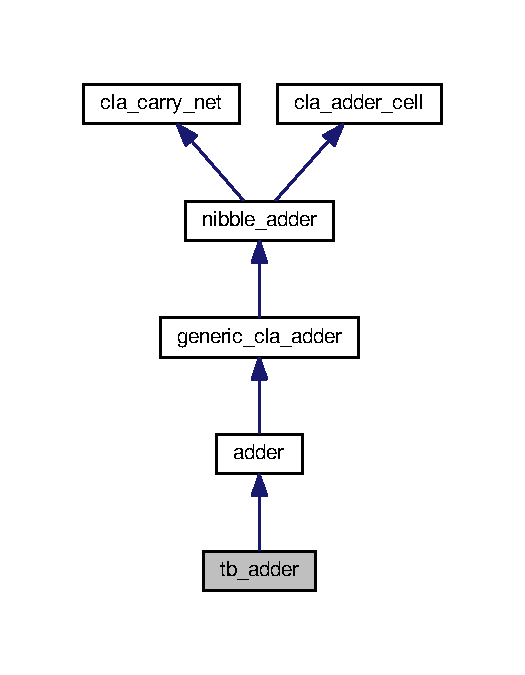
\includegraphics[width=252pt]{classtb__adder__inherit__graph}
\end{center}
\end{figure}


Diagramma di collaborazione per tb\+\_\+adder\+:
\nopagebreak
\begin{figure}[H]
\begin{center}
\leavevmode
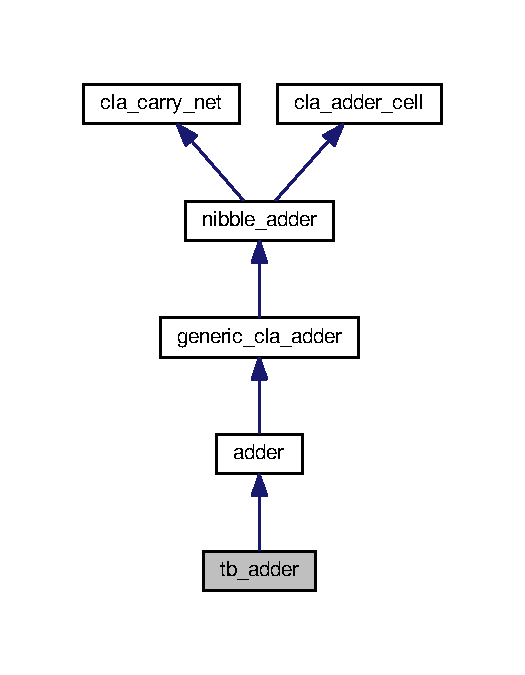
\includegraphics[width=252pt]{classtb__adder__coll__graph}
\end{center}
\end{figure}
\subsection*{Entities}
\begin{DoxyCompactItemize}
\item 
\hyperlink{classtb__adder_1_1behavior}{behavior} architecture
\end{DoxyCompactItemize}


La documentazione per questa classe è stata generata a partire dal seguente file\+:\begin{DoxyCompactItemize}
\item 
Src/adder/\hyperlink{tb__adder_8vhd}{tb\+\_\+adder.\+vhd}\end{DoxyCompactItemize}

\hypertarget{classtb__generic__cla__adder}{\section{tb\+\_\+generic\+\_\+cla\+\_\+adder Entity Reference}
\label{classtb__generic__cla__adder}\index{tb\+\_\+generic\+\_\+cla\+\_\+adder@{tb\+\_\+generic\+\_\+cla\+\_\+adder}}
}


Diagramma delle classi per tb\+\_\+generic\+\_\+cla\+\_\+adder\nopagebreak
\begin{figure}[H]
\begin{center}
\leavevmode
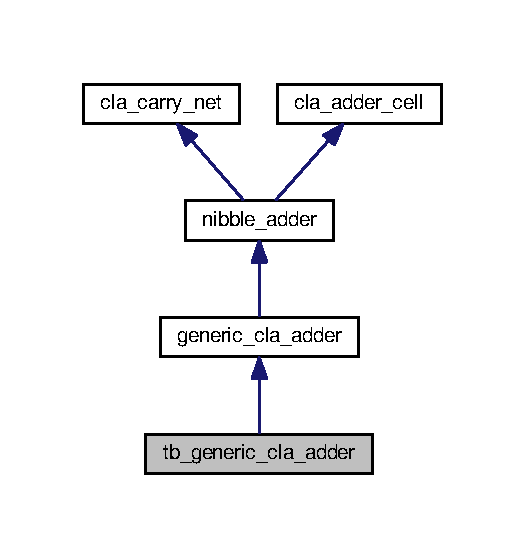
\includegraphics[width=252pt]{classtb__generic__cla__adder__inherit__graph}
\end{center}
\end{figure}


Diagramma di collaborazione per tb\+\_\+generic\+\_\+cla\+\_\+adder\+:\nopagebreak
\begin{figure}[H]
\begin{center}
\leavevmode
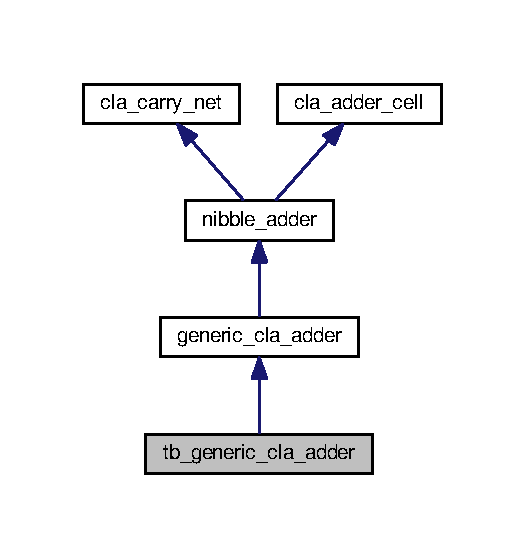
\includegraphics[width=252pt]{classtb__generic__cla__adder__coll__graph}
\end{center}
\end{figure}
\subsection*{Entities}
\begin{DoxyCompactItemize}
\item 
\hyperlink{classtb__generic__cla__adder_1_1behavior}{behavior} architecture
\end{DoxyCompactItemize}


La documentazione per questa classe è stata generata a partire dal seguente file\+:\begin{DoxyCompactItemize}
\item 
Src/adder/\hyperlink{tb__generic__cla__adder_8vhd}{tb\+\_\+generic\+\_\+cla\+\_\+adder.\+vhd}\end{DoxyCompactItemize}

\hypertarget{classtb__prova}{\section{tb\+\_\+prova Entity Reference}
\label{classtb__prova}\index{tb\+\_\+prova@{tb\+\_\+prova}}
}


Diagramma delle classi per tb\+\_\+prova\nopagebreak
\begin{figure}[H]
\begin{center}
\leavevmode
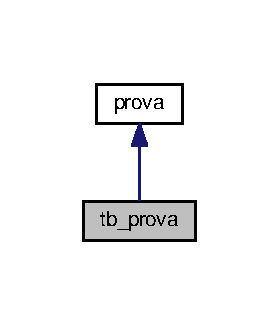
\includegraphics[width=134pt]{classtb__prova__inherit__graph}
\end{center}
\end{figure}


Diagramma di collaborazione per tb\+\_\+prova\+:\nopagebreak
\begin{figure}[H]
\begin{center}
\leavevmode
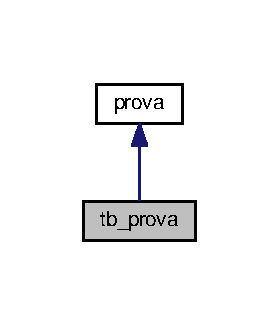
\includegraphics[width=134pt]{classtb__prova__coll__graph}
\end{center}
\end{figure}
\subsection*{Entities}
\begin{DoxyCompactItemize}
\item 
\hyperlink{classtb__prova_1_1_behavioral}{Behavioral} architecture
\end{DoxyCompactItemize}
\subsection*{Libraries}
 \begin{DoxyCompactItemize}
\item 
\hyperlink{classtb__prova_ae4f03c286607f3181e16b9aa12d0c6d4}{I\+E\+E\+E} 
\end{DoxyCompactItemize}
\subsection*{Use Clauses}
 \begin{DoxyCompactItemize}
\item 
\hyperlink{classtb__prova_aa4b2b25246a821511120e3149b003563}{S\+T\+D\+\_\+\+L\+O\+G\+I\+C\+\_\+1164}   
\end{DoxyCompactItemize}


\subsection{Documentazione dei membri dato}
\hypertarget{classtb__prova_ae4f03c286607f3181e16b9aa12d0c6d4}{\index{tb\+\_\+prova@{tb\+\_\+prova}!I\+E\+E\+E@{I\+E\+E\+E}}
\index{I\+E\+E\+E@{I\+E\+E\+E}!tb\+\_\+prova@{tb\+\_\+prova}}
\subsubsection[{I\+E\+E\+E}]{\setlength{\rightskip}{0pt plus 5cm}{\bf I\+E\+E\+E}\hspace{0.3cm}{\ttfamily [Library]}}}\label{classtb__prova_ae4f03c286607f3181e16b9aa12d0c6d4}
\hypertarget{classtb__prova_aa4b2b25246a821511120e3149b003563}{\index{tb\+\_\+prova@{tb\+\_\+prova}!S\+T\+D\+\_\+\+L\+O\+G\+I\+C\+\_\+1164@{S\+T\+D\+\_\+\+L\+O\+G\+I\+C\+\_\+1164}}
\index{S\+T\+D\+\_\+\+L\+O\+G\+I\+C\+\_\+1164@{S\+T\+D\+\_\+\+L\+O\+G\+I\+C\+\_\+1164}!tb\+\_\+prova@{tb\+\_\+prova}}
\subsubsection[{S\+T\+D\+\_\+\+L\+O\+G\+I\+C\+\_\+1164}]{\setlength{\rightskip}{0pt plus 5cm}{\bf S\+T\+D\+\_\+\+L\+O\+G\+I\+C\+\_\+1164}\hspace{0.3cm}{\ttfamily [Package]}}}\label{classtb__prova_aa4b2b25246a821511120e3149b003563}


La documentazione per questa classe è stata generata a partire dal seguente file\+:\begin{DoxyCompactItemize}
\item 
Src/\hyperlink{tb__prova_8vhd}{tb\+\_\+prova.\+vhd}\end{DoxyCompactItemize}

\hypertarget{classtruncate}{\section{truncate Entity Reference}
\label{classtruncate}\index{truncate@{truncate}}
}


Basic\+Fixed\+Point\+Operation @\{  Operazioni fixed-\/point basilari  Truncation @\{  Operazione di troncamento

Tronca un numero signed fixed-\/point di ingresso, espresso in uno specifico formato, restituendone un'equivalente rappresentazione in uno specifico formato di uscita. Per eseguire il troncamento e' necessario conoscere a priori il numero totale di bit usati per la rappresentazione del numero in ingresso ed il numero di bit usati per rappresentare la sua parte intera.  


\subsection*{Entities}
\begin{DoxyCompactItemize}
\item 
\hyperlink{classtruncate_1_1dataflow}{dataflow} architecture
\begin{DoxyCompactList}\small\item\em Implementazione dataflow dell'entity truncate. \end{DoxyCompactList}\end{DoxyCompactItemize}
\subsection*{Generics}
 \begin{DoxyCompactItemize}
\item 
\hyperlink{classtruncate_ad3d18243ad6fe53a2277e2aa9b94ca45}{s\+\_\+in\+\_\+dim} {\bfseries {\bfseries \textcolor{vhdlchar}{integer}\textcolor{vhdlchar}{ }}}
\begin{DoxyCompactList}\small\item\em numero di bit totali su cui e' espresso il segnale di ingresso \end{DoxyCompactList}\item 
\hyperlink{classtruncate_abe72b503b8140ab0d84911165e959b53}{s\+\_\+in\+\_\+int} {\bfseries {\bfseries \textcolor{vhdlchar}{integer}\textcolor{vhdlchar}{ }}}
\begin{DoxyCompactList}\small\item\em numero di bit su cui e' espressa la parte frazionaria del segnale di ingresso \end{DoxyCompactList}\item 
\hyperlink{classtruncate_a8b62f8bfecb0fab845995b8b051101bc}{s\+\_\+out\+\_\+dim} {\bfseries {\bfseries \textcolor{vhdlchar}{integer}\textcolor{vhdlchar}{ }}}
\begin{DoxyCompactList}\small\item\em numero di bit totali su cui e' espresso il segnale di uscita \end{DoxyCompactList}\item 
\hyperlink{classtruncate_a4ca792ca981e2f9d82bf36d9c82c08af}{s\+\_\+out\+\_\+int} {\bfseries {\bfseries \textcolor{vhdlchar}{integer}\textcolor{vhdlchar}{ }}}
\begin{DoxyCompactList}\small\item\em numero di bit su cui e' espressa la parte frazionaria del segnale di uscita \end{DoxyCompactList}\end{DoxyCompactItemize}
\subsection*{Ports}
 \begin{DoxyCompactItemize}
\item 
\hyperlink{classtruncate_a6d6bd3ddfff26c223f1752f25545e304}{s\+\_\+in}  {\bfseries {\bfseries \textcolor{vhdlchar}{in}\textcolor{vhdlchar}{ }}} {\bfseries \textcolor{vhdlchar}{std\+\_\+logic\+\_\+vector}\textcolor{vhdlchar}{ }\textcolor{vhdlchar}{(}\textcolor{vhdlchar}{ }\textcolor{vhdlchar}{ }\textcolor{vhdlchar}{ }\textcolor{vhdlchar}{ }{\bfseries \hyperlink{classtruncate_ad3d18243ad6fe53a2277e2aa9b94ca45}{s\+\_\+in\+\_\+dim}} \textcolor{vhdlchar}{-\/}\textcolor{vhdlchar}{ } \textcolor{vhdldigit}{1} \textcolor{vhdlchar}{ }\textcolor{vhdlchar}{downto}\textcolor{vhdlchar}{ }\textcolor{vhdlchar}{ } \textcolor{vhdldigit}{0} \textcolor{vhdlchar}{ }\textcolor{vhdlchar}{)}\textcolor{vhdlchar}{ }} 
\begin{DoxyCompactList}\small\item\em segnale di ingresso \end{DoxyCompactList}\item 
\hyperlink{classtruncate_a7c0b5e84820296cfa624ce710d19debd}{s\+\_\+out}  {\bfseries {\bfseries \textcolor{vhdlchar}{out}\textcolor{vhdlchar}{ }}} {\bfseries \textcolor{vhdlchar}{std\+\_\+logic\+\_\+vector}\textcolor{vhdlchar}{ }\textcolor{vhdlchar}{(}\textcolor{vhdlchar}{ }\textcolor{vhdlchar}{ }\textcolor{vhdlchar}{ }\textcolor{vhdlchar}{ }{\bfseries \hyperlink{classtruncate_a8b62f8bfecb0fab845995b8b051101bc}{s\+\_\+out\+\_\+dim}} \textcolor{vhdlchar}{ }\textcolor{vhdlchar}{downto}\textcolor{vhdlchar}{ }\textcolor{vhdlchar}{ } \textcolor{vhdldigit}{0} \textcolor{vhdlchar}{ }\textcolor{vhdlchar}{)}\textcolor{vhdlchar}{ }} 
\begin{DoxyCompactList}\small\item\em segnale di uscita, troncato \end{DoxyCompactList}\end{DoxyCompactItemize}


\subsection{Descrizione dettagliata}
Basic\+Fixed\+Point\+Operation @\{  Operazioni fixed-\/point basilari  Truncation @\{  Operazione di troncamento

Tronca un numero signed fixed-\/point di ingresso, espresso in uno specifico formato, restituendone un'equivalente rappresentazione in uno specifico formato di uscita. Per eseguire il troncamento e' necessario conoscere a priori il numero totale di bit usati per la rappresentazione del numero in ingresso ed il numero di bit usati per rappresentare la sua parte intera. 

\subsection{Documentazione dei membri dato}
\hypertarget{classtruncate_a6d6bd3ddfff26c223f1752f25545e304}{\index{truncate@{truncate}!s\+\_\+in@{s\+\_\+in}}
\index{s\+\_\+in@{s\+\_\+in}!truncate@{truncate}}
\subsubsection[{s\+\_\+in}]{\setlength{\rightskip}{0pt plus 5cm}{\bf s\+\_\+in} {\bfseries \textcolor{vhdlchar}{in}\textcolor{vhdlchar}{ }} {\bfseries \textcolor{vhdlchar}{std\+\_\+logic\+\_\+vector}\textcolor{vhdlchar}{ }\textcolor{vhdlchar}{(}\textcolor{vhdlchar}{ }\textcolor{vhdlchar}{ }\textcolor{vhdlchar}{ }\textcolor{vhdlchar}{ }{\bfseries {\bf s\+\_\+in\+\_\+dim}} \textcolor{vhdlchar}{-\/}\textcolor{vhdlchar}{ } \textcolor{vhdldigit}{1} \textcolor{vhdlchar}{ }\textcolor{vhdlchar}{downto}\textcolor{vhdlchar}{ }\textcolor{vhdlchar}{ } \textcolor{vhdldigit}{0} \textcolor{vhdlchar}{ }\textcolor{vhdlchar}{)}\textcolor{vhdlchar}{ }} \hspace{0.3cm}{\ttfamily [Port]}}}\label{classtruncate_a6d6bd3ddfff26c223f1752f25545e304}


segnale di ingresso 

\hypertarget{classtruncate_ad3d18243ad6fe53a2277e2aa9b94ca45}{\index{truncate@{truncate}!s\+\_\+in\+\_\+dim@{s\+\_\+in\+\_\+dim}}
\index{s\+\_\+in\+\_\+dim@{s\+\_\+in\+\_\+dim}!truncate@{truncate}}
\subsubsection[{s\+\_\+in\+\_\+dim}]{\setlength{\rightskip}{0pt plus 5cm}{\bf s\+\_\+in\+\_\+dim} {\bfseries \textcolor{vhdlchar}{ }} {\bfseries \textcolor{vhdlchar}{integer}\textcolor{vhdlchar}{ }} \hspace{0.3cm}{\ttfamily [Generic]}}}\label{classtruncate_ad3d18243ad6fe53a2277e2aa9b94ca45}


numero di bit totali su cui e' espresso il segnale di ingresso 

\hypertarget{classtruncate_abe72b503b8140ab0d84911165e959b53}{\index{truncate@{truncate}!s\+\_\+in\+\_\+int@{s\+\_\+in\+\_\+int}}
\index{s\+\_\+in\+\_\+int@{s\+\_\+in\+\_\+int}!truncate@{truncate}}
\subsubsection[{s\+\_\+in\+\_\+int}]{\setlength{\rightskip}{0pt plus 5cm}{\bf s\+\_\+in\+\_\+int} {\bfseries \textcolor{vhdlchar}{ }} {\bfseries \textcolor{vhdlchar}{integer}\textcolor{vhdlchar}{ }} \hspace{0.3cm}{\ttfamily [Generic]}}}\label{classtruncate_abe72b503b8140ab0d84911165e959b53}


numero di bit su cui e' espressa la parte frazionaria del segnale di ingresso 

\hypertarget{classtruncate_a7c0b5e84820296cfa624ce710d19debd}{\index{truncate@{truncate}!s\+\_\+out@{s\+\_\+out}}
\index{s\+\_\+out@{s\+\_\+out}!truncate@{truncate}}
\subsubsection[{s\+\_\+out}]{\setlength{\rightskip}{0pt plus 5cm}{\bf s\+\_\+out} {\bfseries \textcolor{vhdlchar}{out}\textcolor{vhdlchar}{ }} {\bfseries \textcolor{vhdlchar}{std\+\_\+logic\+\_\+vector}\textcolor{vhdlchar}{ }\textcolor{vhdlchar}{(}\textcolor{vhdlchar}{ }\textcolor{vhdlchar}{ }\textcolor{vhdlchar}{ }\textcolor{vhdlchar}{ }{\bfseries {\bf s\+\_\+out\+\_\+dim}} \textcolor{vhdlchar}{ }\textcolor{vhdlchar}{downto}\textcolor{vhdlchar}{ }\textcolor{vhdlchar}{ } \textcolor{vhdldigit}{0} \textcolor{vhdlchar}{ }\textcolor{vhdlchar}{)}\textcolor{vhdlchar}{ }} \hspace{0.3cm}{\ttfamily [Port]}}}\label{classtruncate_a7c0b5e84820296cfa624ce710d19debd}


segnale di uscita, troncato 

\hypertarget{classtruncate_a8b62f8bfecb0fab845995b8b051101bc}{\index{truncate@{truncate}!s\+\_\+out\+\_\+dim@{s\+\_\+out\+\_\+dim}}
\index{s\+\_\+out\+\_\+dim@{s\+\_\+out\+\_\+dim}!truncate@{truncate}}
\subsubsection[{s\+\_\+out\+\_\+dim}]{\setlength{\rightskip}{0pt plus 5cm}{\bf s\+\_\+out\+\_\+dim} {\bfseries \textcolor{vhdlchar}{ }} {\bfseries \textcolor{vhdlchar}{integer}\textcolor{vhdlchar}{ }} \hspace{0.3cm}{\ttfamily [Generic]}}}\label{classtruncate_a8b62f8bfecb0fab845995b8b051101bc}


numero di bit totali su cui e' espresso il segnale di uscita 

\hypertarget{classtruncate_a4ca792ca981e2f9d82bf36d9c82c08af}{\index{truncate@{truncate}!s\+\_\+out\+\_\+int@{s\+\_\+out\+\_\+int}}
\index{s\+\_\+out\+\_\+int@{s\+\_\+out\+\_\+int}!truncate@{truncate}}
\subsubsection[{s\+\_\+out\+\_\+int}]{\setlength{\rightskip}{0pt plus 5cm}{\bf s\+\_\+out\+\_\+int} {\bfseries \textcolor{vhdlchar}{ }} {\bfseries \textcolor{vhdlchar}{integer}\textcolor{vhdlchar}{ }} \hspace{0.3cm}{\ttfamily [Generic]}}}\label{classtruncate_a4ca792ca981e2f9d82bf36d9c82c08af}


numero di bit su cui e' espressa la parte frazionaria del segnale di uscita 



La documentazione per questa classe è stata generata a partire dal seguente file\+:\begin{DoxyCompactItemize}
\item 
Src/\hyperlink{truncate_8vhd}{truncate.\+vhd}\end{DoxyCompactItemize}

\chapter{Documentazione dei file}
\hypertarget{adder_8vhd}{\section{Riferimenti per il file Src/adder/adder.vhd}
\label{adder_8vhd}\index{Src/adder/adder.\+vhd@{Src/adder/adder.\+vhd}}
}
\subsection*{Entities}
\begin{DoxyCompactItemize}
\item 
\hyperlink{classadder}{adder} entity
\item 
\hyperlink{classadder_1_1structural}{structural} architecture
\end{DoxyCompactItemize}


\subsection{Descrizione dettagliata}
\begin{DoxyAuthor}{Autori}
Salvatore Barone \href{mailto:salvator.barone@gmail.com}{\tt salvator.\+barone@gmail.\+com} ~\newline
 Alfonso Di Martino \href{mailto:alfonsodimartino160989@gmail.com}{\tt alfonsodimartino160989@gmail.\+com} ~\newline
 Sossio Fiorillo \href{mailto:fsossio@gmail.com}{\tt fsossio@gmail.\+com} ~\newline
 Pietro Liguori \href{mailto:pie.liguori@gmail.com}{\tt pie.\+liguori@gmail.\+com} ~\newline

\end{DoxyAuthor}
\begin{DoxyDate}{Data}
01 07 2017
\end{DoxyDate}
\begin{DoxyCopyright}{Copyright}
Copyright 2017 Salvatore Barone \href{mailto:salvator.barone@gmail.com}{\tt salvator.\+barone@gmail.\+com} ~\newline
 Alfonso Di Martino \href{mailto:alfonsodimartino160989@gmail.com}{\tt alfonsodimartino160989@gmail.\+com} ~\newline
 Sossio Fiorillo \href{mailto:fsossio@gmail.com}{\tt fsossio@gmail.\+com} ~\newline
 Pietro Liguori \href{mailto:pie.liguori@gmail.com}{\tt pie.\+liguori@gmail.\+com} ~\newline

\end{DoxyCopyright}
This file is part of Linear-\/\+Regression.

Linear-\/\+Regression is free software; you can redistribute it and/or modify it under the terms of the G\+N\+U General Public License as published by the Free Software Foundation; either version 3 of the License, or any later version.

Linear-\/\+Regression is distributed in the hope that it will be useful, but W\+I\+T\+H\+O\+U\+T A\+N\+Y W\+A\+R\+R\+A\+N\+T\+Y; without even the implied warranty of M\+E\+R\+C\+H\+A\+N\+T\+A\+B\+I\+L\+I\+T\+Y or F\+I\+T\+N\+E\+S\+S F\+O\+R A P\+A\+R\+T\+I\+C\+U\+L\+A\+R P\+U\+R\+P\+O\+S\+E. See the G\+N\+U General Public License for more details.

You should have received a copy of the G\+N\+U General Public License along with this program; if not, write to the Free Software Foundation, Inc., 51 Franklin Street, Fifth Floor, Boston, M\+A 02110-\/1301, U\+S\+A. 
\hypertarget{cla__adder__cell_8vhd}{\section{Riferimenti per il file Src/adder/cla\+\_\+adder\+\_\+cell.vhd}
\label{cla__adder__cell_8vhd}\index{Src/adder/cla\+\_\+adder\+\_\+cell.\+vhd@{Src/adder/cla\+\_\+adder\+\_\+cell.\+vhd}}
}
\subsection*{Entities}
\begin{DoxyCompactItemize}
\item 
\hyperlink{classcla__adder__cell}{cla\+\_\+adder\+\_\+cell} entity
\begin{DoxyCompactList}\small\item\em Cella base di un addizionatore con carry-\/lookahead.

La cella somma tra loro due addendi ed un carry in ingresso, tutti espressi su un solo bit. Oltre a generare la somma, genera le funzioni \char`\"{}propagazione\char`\"{} e \char`\"{}generazione\char`\"{} del carry. \end{DoxyCompactList}\item 
\hyperlink{classcla__adder__cell_1_1dataflow}{dataflow} architecture
\end{DoxyCompactItemize}


\subsection{Descrizione dettagliata}
\begin{DoxyAuthor}{Autori}
Salvatore Barone \href{mailto:salvator.barone@gmail.com}{\tt salvator.\+barone@gmail.\+com} ~\newline
 Alfonso Di Martino \href{mailto:alfonsodimartino160989@gmail.com}{\tt alfonsodimartino160989@gmail.\+com} ~\newline
 Sossio Fiorillo \href{mailto:fsossio@gmail.com}{\tt fsossio@gmail.\+com} ~\newline
 Pietro Liguori \href{mailto:pie.liguori@gmail.com}{\tt pie.\+liguori@gmail.\+com} ~\newline

\end{DoxyAuthor}
\begin{DoxyDate}{Data}
01 07 2017
\end{DoxyDate}
\begin{DoxyCopyright}{Copyright}
Copyright 2017 Salvatore Barone \href{mailto:salvator.barone@gmail.com}{\tt salvator.\+barone@gmail.\+com} ~\newline
 Alfonso Di Martino \href{mailto:alfonsodimartino160989@gmail.com}{\tt alfonsodimartino160989@gmail.\+com} ~\newline
 Sossio Fiorillo \href{mailto:fsossio@gmail.com}{\tt fsossio@gmail.\+com} ~\newline
 Pietro Liguori \href{mailto:pie.liguori@gmail.com}{\tt pie.\+liguori@gmail.\+com} ~\newline

\end{DoxyCopyright}
This file is part of Linear-\/\+Regression.

Linear-\/\+Regression is free software; you can redistribute it and/or modify it under the terms of the G\+N\+U General Public License as published by the Free Software Foundation; either version 3 of the License, or any later version.

Linear-\/\+Regression is distributed in the hope that it will be useful, but W\+I\+T\+H\+O\+U\+T A\+N\+Y W\+A\+R\+R\+A\+N\+T\+Y; without even the implied warranty of M\+E\+R\+C\+H\+A\+N\+T\+A\+B\+I\+L\+I\+T\+Y or F\+I\+T\+N\+E\+S\+S F\+O\+R A P\+A\+R\+T\+I\+C\+U\+L\+A\+R P\+U\+R\+P\+O\+S\+E. See the G\+N\+U General Public License for more details.

You should have received a copy of the G\+N\+U General Public License along with this program; if not, write to the Free Software Foundation, Inc., 51 Franklin Street, Fifth Floor, Boston, M\+A 02110-\/1301, U\+S\+A. 
\hypertarget{cla__carry__net_8vhd}{\section{Riferimenti per il file Src/adder/cla\+\_\+carry\+\_\+net.vhd}
\label{cla__carry__net_8vhd}\index{Src/adder/cla\+\_\+carry\+\_\+net.\+vhd@{Src/adder/cla\+\_\+carry\+\_\+net.\+vhd}}
}
\subsection*{Entities}
\begin{DoxyCompactItemize}
\item 
\hyperlink{classcla__carry__net}{cla\+\_\+carry\+\_\+net} entity
\begin{DoxyCompactList}\small\item\em Rete logica di calcolo dei riporti per un addizionatore a quattro bit con carry lookahead.

Permette di anticipare il calcolo dei riporti usando le funzioni \char`\"{}propagazione\char`\"{} e \char`\"{}generazione\char`\"{} prodotte dai singoli blocchi \hyperlink{classcla__adder__cell}{cla\+\_\+adder\+\_\+cell}, in modo da ridurre tempo necessario ad effettuare il calcolo di tutti i carry, quindi il tempo necessario a completare la somma. Questo blocco calcola solo i carry, pertanto va connesso ai blocchi \hyperlink{classcla__adder__cell}{cla\+\_\+adder\+\_\+cell}, per il calcolo materiale della somma, così come indicato dallo schema seguente, il quale rappresenta lo schema completo di un addizionatore a quattro bit\+: . \end{DoxyCompactList}\item 
\hyperlink{classcla__carry__net_1_1dataflow}{dataflow} architecture
\begin{DoxyCompactList}\small\item\em Implementazione dataflow dell'entita' \hyperlink{classcla__carry__net}{cla\+\_\+carry\+\_\+net}. \end{DoxyCompactList}\end{DoxyCompactItemize}


\subsection{Descrizione dettagliata}
\begin{DoxyAuthor}{Autori}
Salvatore Barone \href{mailto:salvator.barone@gmail.com}{\tt salvator.\+barone@gmail.\+com} ~\newline
 Alfonso Di Martino \href{mailto:alfonsodimartino160989@gmail.com}{\tt alfonsodimartino160989@gmail.\+com} ~\newline
 Sossio Fiorillo \href{mailto:fsossio@gmail.com}{\tt fsossio@gmail.\+com} ~\newline
 Pietro Liguori \href{mailto:pie.liguori@gmail.com}{\tt pie.\+liguori@gmail.\+com} ~\newline

\end{DoxyAuthor}
\begin{DoxyDate}{Data}
01 07 2017
\end{DoxyDate}
\begin{DoxyCopyright}{Copyright}
Copyright 2017 Salvatore Barone \href{mailto:salvator.barone@gmail.com}{\tt salvator.\+barone@gmail.\+com} ~\newline
 Alfonso Di Martino \href{mailto:alfonsodimartino160989@gmail.com}{\tt alfonsodimartino160989@gmail.\+com} ~\newline
 Sossio Fiorillo \href{mailto:fsossio@gmail.com}{\tt fsossio@gmail.\+com} ~\newline
 Pietro Liguori \href{mailto:pie.liguori@gmail.com}{\tt pie.\+liguori@gmail.\+com} ~\newline

\end{DoxyCopyright}
This file is part of Linear-\/\+Regression.

Linear-\/\+Regression is free software; you can redistribute it and/or modify it under the terms of the G\+N\+U General Public License as published by the Free Software Foundation; either version 3 of the License, or any later version.

Linear-\/\+Regression is distributed in the hope that it will be useful, but W\+I\+T\+H\+O\+U\+T A\+N\+Y W\+A\+R\+R\+A\+N\+T\+Y; without even the implied warranty of M\+E\+R\+C\+H\+A\+N\+T\+A\+B\+I\+L\+I\+T\+Y or F\+I\+T\+N\+E\+S\+S F\+O\+R A P\+A\+R\+T\+I\+C\+U\+L\+A\+R P\+U\+R\+P\+O\+S\+E. See the G\+N\+U General Public License for more details.

You should have received a copy of the G\+N\+U General Public License along with this program; if not, write to the Free Software Foundation, Inc., 51 Franklin Street, Fifth Floor, Boston, M\+A 02110-\/1301, U\+S\+A. 
\hypertarget{generic__cla__adder_8vhd}{\section{Riferimenti per il file Src/adder/generic\+\_\+cla\+\_\+adder.vhd}
\label{generic__cla__adder_8vhd}\index{Src/adder/generic\+\_\+cla\+\_\+adder.\+vhd@{Src/adder/generic\+\_\+cla\+\_\+adder.\+vhd}}
}
\subsection*{Entities}
\begin{DoxyCompactItemize}
\item 
\hyperlink{classgeneric__cla__adder}{generic\+\_\+cla\+\_\+adder} entity
\begin{DoxyCompactList}\small\item\em Adder custom con carry-\/lookahead

\hyperlink{classgeneric__cla__adder}{generic\+\_\+cla\+\_\+adder} somma tra loro due addendi ed un carry in ingresso; gli addendi sono espressi su multipli interi di quattro bit. Oltre a generare la somma, genera il flag di carry ed il flag di overflow. \end{DoxyCompactList}\item 
\hyperlink{classgeneric__cla__adder_1_1structural}{structural} architecture
\begin{DoxyCompactList}\small\item\em Implementazione structural di \hyperlink{classgeneric__cla__adder}{generic\+\_\+cla\+\_\+adder}. \end{DoxyCompactList}\end{DoxyCompactItemize}


\subsection{Descrizione dettagliata}
\begin{DoxyAuthor}{Autori}
Salvatore Barone \href{mailto:salvator.barone@gmail.com}{\tt salvator.\+barone@gmail.\+com} ~\newline
 Alfonso Di Martino \href{mailto:alfonsodimartino160989@gmail.com}{\tt alfonsodimartino160989@gmail.\+com} ~\newline
 Sossio Fiorillo \href{mailto:fsossio@gmail.com}{\tt fsossio@gmail.\+com} ~\newline
 Pietro Liguori \href{mailto:pie.liguori@gmail.com}{\tt pie.\+liguori@gmail.\+com} ~\newline

\end{DoxyAuthor}
\begin{DoxyDate}{Data}
01 07 2017
\end{DoxyDate}
\begin{DoxyCopyright}{Copyright}
Copyright 2017 Salvatore Barone \href{mailto:salvator.barone@gmail.com}{\tt salvator.\+barone@gmail.\+com} ~\newline
 Alfonso Di Martino \href{mailto:alfonsodimartino160989@gmail.com}{\tt alfonsodimartino160989@gmail.\+com} ~\newline
 Sossio Fiorillo \href{mailto:fsossio@gmail.com}{\tt fsossio@gmail.\+com} ~\newline
 Pietro Liguori \href{mailto:pie.liguori@gmail.com}{\tt pie.\+liguori@gmail.\+com} ~\newline

\end{DoxyCopyright}
This file is part of Linear-\/\+Regression.

Linear-\/\+Regression is free software; you can redistribute it and/or modify it under the terms of the G\+N\+U General Public License as published by the Free Software Foundation; either version 3 of the License, or any later version.

Linear-\/\+Regression is distributed in the hope that it will be useful, but W\+I\+T\+H\+O\+U\+T A\+N\+Y W\+A\+R\+R\+A\+N\+T\+Y; without even the implied warranty of M\+E\+R\+C\+H\+A\+N\+T\+A\+B\+I\+L\+I\+T\+Y or F\+I\+T\+N\+E\+S\+S F\+O\+R A P\+A\+R\+T\+I\+C\+U\+L\+A\+R P\+U\+R\+P\+O\+S\+E. See the G\+N\+U General Public License for more details.

You should have received a copy of the G\+N\+U General Public License along with this program; if not, write to the Free Software Foundation, Inc., 51 Franklin Street, Fifth Floor, Boston, M\+A 02110-\/1301, U\+S\+A. 
\hypertarget{nibble__adder_8vhd}{}\section{Riferimenti per il file Src/adder/nibble\+\_\+adder.vhd}
\label{nibble__adder_8vhd}\index{Src/adder/nibble\+\_\+adder.\+vhd@{Src/adder/nibble\+\_\+adder.\+vhd}}
\subsection*{Entities}
\begin{DoxyCompactItemize}
\item 
\hyperlink{classnibble__adder}{nibble\+\_\+adder} entity
\begin{DoxyCompactList}\small\item\em Addizionatore con carry-\/lookahead a quattro bit.

La cella somma tra loro due addendi ed un carry in ingresso; gli addendi sono espressi su quattro bit. Oltre a generare la somma, genera le funzioni \char`\"{}propagazione\char`\"{} e \char`\"{}generazione\char`\"{} del carry per eventuali blocchi \hyperlink{classnibble__adder}{nibble\+\_\+adder} posti a valle. \end{DoxyCompactList}\item 
\hyperlink{classnibble__adder_1_1structural}{structural} architecture
\begin{DoxyCompactList}\small\item\em Implementazione structural dell\textquotesingle{}entità \hyperlink{classnibble__adder}{nibble\+\_\+adder}.

Questa architettura istanzia una entità \hyperlink{classcla__carry__net}{cla\+\_\+carry\+\_\+net} ed una entità \hyperlink{classcla__adder__cell}{cla\+\_\+adder\+\_\+cell} per ogni bit su cui sono espressi gli addendi, connettendoli tra loro secondo lo schema riportato di seguito\+: . \end{DoxyCompactList}\end{DoxyCompactItemize}


\subsection{Descrizione dettagliata}
\begin{DoxyAuthor}{Autori}
Salvatore Barone \href{mailto:salvator.barone@gmail.com}{\tt salvator.\+barone@gmail.\+com} ~\newline
 Alfonso Di Martino \href{mailto:alfonsodimartino160989@gmail.com}{\tt alfonsodimartino160989@gmail.\+com} ~\newline
 Sossio Fiorillo \href{mailto:fsossio@gmail.com}{\tt fsossio@gmail.\+com} ~\newline
 Pietro Liguori \href{mailto:pie.liguori@gmail.com}{\tt pie.\+liguori@gmail.\+com} ~\newline

\end{DoxyAuthor}
\begin{DoxyDate}{Data}
01 07 2017
\end{DoxyDate}
\begin{DoxyCopyright}{Copyright}
Copyright 2017 Salvatore Barone \href{mailto:salvator.barone@gmail.com}{\tt salvator.\+barone@gmail.\+com} ~\newline
 Alfonso Di Martino \href{mailto:alfonsodimartino160989@gmail.com}{\tt alfonsodimartino160989@gmail.\+com} ~\newline
 Sossio Fiorillo \href{mailto:fsossio@gmail.com}{\tt fsossio@gmail.\+com} ~\newline
 Pietro Liguori \href{mailto:pie.liguori@gmail.com}{\tt pie.\+liguori@gmail.\+com} ~\newline

\end{DoxyCopyright}
This file is part of Linear-\/\+Regression.

Linear-\/\+Regression is free software; you can redistribute it and/or modify it under the terms of the G\+NU General Public License as published by the Free Software Foundation; either version 3 of the License, or any later version.

Linear-\/\+Regression is distributed in the hope that it will be useful, but W\+I\+T\+H\+O\+UT A\+NY W\+A\+R\+R\+A\+N\+TY; without even the implied warranty of M\+E\+R\+C\+H\+A\+N\+T\+A\+B\+I\+L\+I\+TY or F\+I\+T\+N\+E\+SS F\+OR A P\+A\+R\+T\+I\+C\+U\+L\+AR P\+U\+R\+P\+O\+SE. See the G\+NU General Public License for more details.

You should have received a copy of the G\+NU General Public License along with this program; if not, write to the Free Software Foundation, Inc., 51 Franklin Street, Fifth Floor, Boston, MA 02110-\/1301, U\+SA. 
\hypertarget{tb__adder_8vhd}{}\section{Riferimenti per il file Src/adder/tb\+\_\+adder.vhd}
\label{tb__adder_8vhd}\index{Src/adder/tb\+\_\+adder.\+vhd@{Src/adder/tb\+\_\+adder.\+vhd}}
\subsection*{Entities}
\begin{DoxyCompactItemize}
\item 
\hyperlink{classtb__adder}{tb\+\_\+adder} entity
\item 
\hyperlink{classtb__adder_1_1behavior}{behavior} architecture
\end{DoxyCompactItemize}


\subsection{Descrizione dettagliata}
\begin{DoxyAuthor}{Autori}
Salvatore Barone \href{mailto:salvator.barone@gmail.com}{\tt salvator.\+barone@gmail.\+com} ~\newline
 Alfonso Di Martino \href{mailto:alfonsodimartino160989@gmail.com}{\tt alfonsodimartino160989@gmail.\+com} ~\newline
 Sossio Fiorillo \href{mailto:fsossio@gmail.com}{\tt fsossio@gmail.\+com} ~\newline
 Pietro Liguori \href{mailto:pie.liguori@gmail.com}{\tt pie.\+liguori@gmail.\+com} ~\newline

\end{DoxyAuthor}
\begin{DoxyDate}{Data}
01 07 2017
\end{DoxyDate}
\begin{DoxyCopyright}{Copyright}
Copyright 2017 Salvatore Barone \href{mailto:salvator.barone@gmail.com}{\tt salvator.\+barone@gmail.\+com} ~\newline
 Alfonso Di Martino \href{mailto:alfonsodimartino160989@gmail.com}{\tt alfonsodimartino160989@gmail.\+com} ~\newline
 Sossio Fiorillo \href{mailto:fsossio@gmail.com}{\tt fsossio@gmail.\+com} ~\newline
 Pietro Liguori \href{mailto:pie.liguori@gmail.com}{\tt pie.\+liguori@gmail.\+com} ~\newline

\end{DoxyCopyright}
This file is part of Linear-\/\+Regression.

Linear-\/\+Regression is free software; you can redistribute it and/or modify it under the terms of the G\+NU General Public License as published by the Free Software Foundation; either version 3 of the License, or any later version.

Linear-\/\+Regression is distributed in the hope that it will be useful, but W\+I\+T\+H\+O\+UT A\+NY W\+A\+R\+R\+A\+N\+TY; without even the implied warranty of M\+E\+R\+C\+H\+A\+N\+T\+A\+B\+I\+L\+I\+TY or F\+I\+T\+N\+E\+SS F\+OR A P\+A\+R\+T\+I\+C\+U\+L\+AR P\+U\+R\+P\+O\+SE. See the G\+NU General Public License for more details.

You should have received a copy of the G\+NU General Public License along with this program; if not, write to the Free Software Foundation, Inc., 51 Franklin Street, Fifth Floor, Boston, MA 02110-\/1301, U\+SA. 
\hypertarget{tb__generic__cla__adder_8vhd}{}\section{Riferimenti per il file Src/adder/tb\+\_\+generic\+\_\+cla\+\_\+adder.vhd}
\label{tb__generic__cla__adder_8vhd}\index{Src/adder/tb\+\_\+generic\+\_\+cla\+\_\+adder.\+vhd@{Src/adder/tb\+\_\+generic\+\_\+cla\+\_\+adder.\+vhd}}
\subsection*{Entities}
\begin{DoxyCompactItemize}
\item 
\hyperlink{classtb__generic__cla__adder}{tb\+\_\+generic\+\_\+cla\+\_\+adder} entity
\item 
\hyperlink{classtb__generic__cla__adder_1_1behavior}{behavior} architecture
\end{DoxyCompactItemize}


\subsection{Descrizione dettagliata}
\begin{DoxyAuthor}{Autori}
Salvatore Barone \href{mailto:salvator.barone@gmail.com}{\tt salvator.\+barone@gmail.\+com} ~\newline
 Alfonso Di Martino \href{mailto:alfonsodimartino160989@gmail.com}{\tt alfonsodimartino160989@gmail.\+com} ~\newline
 Sossio Fiorillo \href{mailto:fsossio@gmail.com}{\tt fsossio@gmail.\+com} ~\newline
 Pietro Liguori \href{mailto:pie.liguori@gmail.com}{\tt pie.\+liguori@gmail.\+com} ~\newline

\end{DoxyAuthor}
\begin{DoxyDate}{Data}
01 07 2017
\end{DoxyDate}
\begin{DoxyCopyright}{Copyright}
Copyright 2017 Salvatore Barone \href{mailto:salvator.barone@gmail.com}{\tt salvator.\+barone@gmail.\+com} ~\newline
 Alfonso Di Martino \href{mailto:alfonsodimartino160989@gmail.com}{\tt alfonsodimartino160989@gmail.\+com} ~\newline
 Sossio Fiorillo \href{mailto:fsossio@gmail.com}{\tt fsossio@gmail.\+com} ~\newline
 Pietro Liguori \href{mailto:pie.liguori@gmail.com}{\tt pie.\+liguori@gmail.\+com} ~\newline

\end{DoxyCopyright}
This file is part of Linear-\/\+Regression.

Linear-\/\+Regression is free software; you can redistribute it and/or modify it under the terms of the G\+NU General Public License as published by the Free Software Foundation; either version 3 of the License, or any later version.

Linear-\/\+Regression is distributed in the hope that it will be useful, but W\+I\+T\+H\+O\+UT A\+NY W\+A\+R\+R\+A\+N\+TY; without even the implied warranty of M\+E\+R\+C\+H\+A\+N\+T\+A\+B\+I\+L\+I\+TY or F\+I\+T\+N\+E\+SS F\+OR A P\+A\+R\+T\+I\+C\+U\+L\+AR P\+U\+R\+P\+O\+SE. See the G\+NU General Public License for more details.

You should have received a copy of the G\+NU General Public License along with this program; if not, write to the Free Software Foundation, Inc., 51 Franklin Street, Fifth Floor, Boston, MA 02110-\/1301, U\+SA. 
\hypertarget{prova_8vhd}{\section{Riferimenti per il file Src/prova.vhd}
\label{prova_8vhd}\index{Src/prova.\+vhd@{Src/prova.\+vhd}}
}
\subsection*{Entities}
\begin{DoxyCompactItemize}
\item 
\hyperlink{classprova}{prova} entity
\item 
\hyperlink{classprova_1_1_behavioral}{Behavioral} architecture
\end{DoxyCompactItemize}

\hypertarget{tb__prova_8vhd}{\section{Riferimenti per il file Src/tb\+\_\+prova.vhd}
\label{tb__prova_8vhd}\index{Src/tb\+\_\+prova.\+vhd@{Src/tb\+\_\+prova.\+vhd}}
}
\subsection*{Entities}
\begin{DoxyCompactItemize}
\item 
\hyperlink{classtb__prova}{tb\+\_\+prova} entity
\item 
\hyperlink{classtb__prova_1_1_behavioral}{Behavioral} architecture
\end{DoxyCompactItemize}

\hypertarget{truncate_8vhd}{\section{Src/truncate.vhd File Reference}
\label{truncate_8vhd}\index{Src/truncate.\+vhd@{Src/truncate.\+vhd}}
}
\subsection*{Entities}
\begin{DoxyCompactItemize}
\item 
\hyperlink{classtruncate}{truncate} entity
\begin{DoxyCompactList}\small\item\em Basic\+Fixed\+Point\+Operation @\{  Operazioni fixed-\/point basilari  Truncation @\{  Operazione di troncamento

Tronca un numero signed fixed-\/point di ingresso, espresso in uno specifico formato, restituendone un'equivalente rappresentazione in uno specifico formato di uscita. Per eseguire il troncamento e' necessario conoscere a priori il numero totale di bit usati per la rappresentazione del numero in ingresso ed il numero di bit usati per rappresentare la sua parte intera. \end{DoxyCompactList}\item 
\hyperlink{classtruncate_1_1dataflow}{dataflow} architecture
\begin{DoxyCompactList}\small\item\em Implementazione dataflow dell'entity truncate. \end{DoxyCompactList}\end{DoxyCompactItemize}


\subsection{Detailed Description}
\begin{DoxyAuthor}{Authors}
Salvatore Barone \href{mailto:salvator.barone@gmail.com}{\tt salvator.\+barone@gmail.\+com} ~\newline
 Alfonso Di Martino \href{mailto:alfonsodimartino160989@gmail.com}{\tt alfonsodimartino160989@gmail.\+com} ~\newline
 Sossio Fiorillo \href{mailto:fsossio@gmail.com}{\tt fsossio@gmail.\+com} ~\newline
 Pietro Liguori \href{mailto:pie.liguori@gmail.com}{\tt pie.\+liguori@gmail.\+com} ~\newline

\end{DoxyAuthor}
\begin{DoxyDate}{Date}
29 06 2017
\end{DoxyDate}
\begin{DoxyCopyright}{Copyright}
Copyright 2017 Salvatore Barone \href{mailto:salvator.barone@gmail.com}{\tt salvator.\+barone@gmail.\+com} ~\newline
 Alfonso Di Martino \href{mailto:alfonsodimartino160989@gmail.com}{\tt alfonsodimartino160989@gmail.\+com} ~\newline
 Sossio Fiorillo \href{mailto:fsossio@gmail.com}{\tt fsossio@gmail.\+com} ~\newline
 Pietro Liguori \href{mailto:pie.liguori@gmail.com}{\tt pie.\+liguori@gmail.\+com} ~\newline

\end{DoxyCopyright}
This file is part of Linear-\/\+Regression.

Linear-\/\+Regression is free software; you can redistribute it and/or modify it under the terms of the G\+N\+U General Public License as published by the Free Software Foundation; either version 3 of the License, or any later version.

Linear-\/\+Regression is distributed in the hope that it will be useful, but W\+I\+T\+H\+O\+U\+T A\+N\+Y W\+A\+R\+R\+A\+N\+T\+Y; without even the implied warranty of M\+E\+R\+C\+H\+A\+N\+T\+A\+B\+I\+L\+I\+T\+Y or F\+I\+T\+N\+E\+S\+S F\+O\+R A P\+A\+R\+T\+I\+C\+U\+L\+A\+R P\+U\+R\+P\+O\+S\+E. See the G\+N\+U General Public License for more details.

You should have received a copy of the G\+N\+U General Public License along with this program; if not, write to the Free Software Foundation, Inc., 51 Franklin Street, Fifth Floor, Boston, M\+A 02110-\/1301, U\+S\+A. 
%--- End generated contents ---

% Index
\newpage
\phantomsection
\addcontentsline{toc}{chapter}{Indice}
\printindex

\end{document}
